% ============================================================
%  第八章 能带论（§1–§11 + 章末参考文献）
%  底本：高等教育出版社《固体理论》第二版；原书印刷页 287–342
%  （PDF 页 = 印刷页 + 20）
%  公式编号自检：§1 (8.1.1)–(8.1.13)；§2 (8.2.1)–(8.2.17)；
%    §3 (8.3.1)–(8.3.21)；§4 (8.4.1)–(8.4.10)；§5 (8.5.1)–(8.5.44)；
%    §6 (8.6.1)–(8.6.25)；§7 (8.7.1)–(8.7.16)；§8 (8.8.1)–(8.8.30)；
%    §9 (8.9.1)–(8.9.25)；§10 (8.10.1)–(8.10.25)；
%    §11 (8.11.1)–(8.11.54)（其中 (8.11.8a/b)、(8.11.9a/b)、
%    (8.11.11a/b/c)、(8.11.20a–d)、(8.11.21a/b)、(8.11.22a/b)、
%    (8.11.25a/b/c)、(8.11.27a/b) 为原书自带二级编号，用
%    subequations 环境照录，与 ch04/ch06 体例一致）。
%    全章自动编号共 280 个编号公式。
%
%  任务单所列 13 处"缺号"逐条对照原书页面判定（均非原书跳号，
%  公式全部在原书中，只是 OCR 的 tag 残缺或粘连，已按页面归位）：
%    (8.2.7)  原书 p291 在号（OCR tag 残为 {2.7}）；
%    (8.2.12) 原书 p292 在号（OCR tag 残为"( 8 ."）；
%    (8.2.13) 原书 p292 在号，OCR 的 tag {8.2.13} 本就完整，不缺；
%    (8.3.13) 原书 p296 在号（p296 顶五行连等式），OCR 漏 tag 且
%             公式严重乱码，已按 p296 重排；
%    (8.6.6)  原书 p309 在号（编号 OCR 掉为正文行"（8.6.6）"）；
%    (8.6.7)  原书 p309 在号（OCR tag 残为 {6.7}）；
%    (8.6.15) 原书 p310 在号（OCR tag 残为 {6.15}）；
%    (8.6.24) 原书 p312 在号，OCR 的 tag 本就完整，不缺；
%    (8.8.13) 原书 p318 在号（OCR tag 残为 {8.13}）；
%    (8.9.5)  原书 p321 在号（编号 OCR 粘进公式末行）；
%    (8.10.8) 原书 p326 在号（OCR tag 残为 {10.8}）。
%
%  已修正的 OCR/原书错误（除全角句点转"."、删 ~ 间隔符、收紧
%  \mathrm{d}、拆开行内公式与中文等常规项外）：
%  1. §1 (8.1.3) 求和下标按原书为倒格矢 K（OCR 误作 k）；
%     (8.1.7)"(N2)^{-1/2}"→(NΩ)^{-1/2}；(8.1.11) 系数 a(k+K')
%     系原书排印如此（投影后指标未换），照录（p288）。
%  2. 表 8.1 表头"k_r = 0.589"→k_F = 0.589、"a(X)"→a(K)，各列
%     数据按 p288–289 复核；正文中"不同 1KI 值"→|K| 值、"A1"→Al。
%  3. §2 (8.2.9)"O_{1-}Σ<ψ_c|ψ_{c'}>"→(1-Σ_{c'}<ψ_c|ψ_{c'}>)（p291）；
%     (8.2.16)(8.2.17) 及其间三个未编号矩阵元式按 p293 重排，
%     (8.2.17) 末尾 OCR 脱落的因子 ×(ℏ²k²/2m + |E_{1s}|) 按 p293 补回。
%  4. §3.1"综上所述"→"综合上述"（p295）；p295 脚注①"因为离子实中
%     壳层电子波函数是振荡的……否则两者不能正交."OCR 漏失，按页脚补录。
%  5. §3.2 (8.3.9)–(8.3.12) 及 (8.3.13) 五行连等式按 p295–296 重排；
%     (8.3.14) 左矢按 p296 为 <ψ_k|（OCR 误作 φ_k）。
%  6. §3.3"光谱项一 a_M 致"→"光谱项一致"（OCR 衍字倒装，p298）；
%     (8.6.1) 第二分段条件"r≠r_i"→"r⩾r_i"（p309，丸盒势球外为零）。
%  7. §4 (8.4.2)(8.4.4)(8.4.7) 的 χ/χ_k 乱码按 p299–300 重排；
%     (8.4.7) OCR 拆成的两块按原书合并为一式（p299–300 跨页一式）；
%     正文"平滑的 x"→"平滑的 χ_k"（p299）。
%  8. §5 (8.5.9) r_。→r_s；(8.5.16)"d/r dτ"→(1/r)dτ（p304）；
%     (8.5.17) 前"α = m/m*"→α≡m/m*（p304）；"球形近P似"→"球形近似"；
%     (8.5.23) r_1 ≡ r/r 照录（r_1 为 r 方向单位矢）；
%     (8.5.25)(8.5.28) OCR 的 τ 按 p305 原书统一为 r；
%     "反映操作"→"反演操作"（p305，u_1 为奇函数）。
%  9. §5 图 8.6 图注 OCR 粘进行文（"自由原子状态(实线)和金属态
%     (虚线)时波函数的示意图"），按 p304 拆出；其前文按 p304 补回
%     "离子实势.图 8.6 是 Na 的 3s 电子在"；"(8:5.12)"→(8.5.12)；
%     φ_0→ψ_0（p304）。
% 10. §6 丸盒势"muffin-tin potential"粘连已拆；(8.6.2)(8.6.5) 按
%     p309 复核；(8.6.9)"E·{ψ_k}∫φ_k*ψ_kdτ"→E[ψ_k]∫ψ_k*ψ_kdτ
%     （p309）；(8.6.17)(8.6.18)(8.6.23) 中球贝塞尔函数下标按 p310
%     原书为 j_1（OCR 误作 j_l）。
% 11. §7 (8.7.5) 求和指标按 p313 为 j（OCR 误作 l）；
%     (8.7.12) OCR 拆成的两块按原书合并为一式（p315）；
%     (8.7.15)(8.7.16) 按 p315 复核；p315 脚注①（里德伯原子单位）
%     OCR 漏失，按页脚补录；"KKR法："→"KKR法."（p313）。
% 12. §8 (8.8.4)(8.8.6)(8.8.17)(8.8.18) 及未编号算符关系式中的
%     φ_{nk}→ψ_{nk}（p317–319）；(8.8.13) 按 p318 重排；
%     (8.8.22) 第二行按 p319 复原为 C_{lσ}、C⁺_{lσ}（k∈BZ 求和）。
% 13. §9 (8.9.1) OCR 拆成的两块按原书合并为一式（p321，原书两行
%     共一号）；(8.9.5) 四行连等式按 p321 重排；
%     (8.9.13) 中 {\dot R}²→ℏ²（OCR 乱码，p322）；
%     (8.9.23) tag"8.9,23"归位；正文"电离能 1E_1|"→|E_1|；
%     "Ge、Si 中的 Ge 施主能级"衍字"Ge"已删（p324）；
%     (8.9.25) 原书排印"-(1/ℏ)F·(1/ℏ)∇_k f"第二个 1/ℏ 为衍余
%     （与 (8.9.24) 比较），已删并注（p324）。
% 14. §10 (8.10.1) 左端按 p325 为 ψ_{nk}(r)（OCR 误作 φ_{nk}）；
%     (8.10.8) tag 残缺归还本式；(8.10.13)(8.10.15) 中 φ/ψ 按
%     p326–327 照录；(8.10.25) 左端按 p329 为 E(k)。
% 15. §11 (8.11.8a/b)–(8.11.53) 各块乱码按 p330–341 重排复原；
%     (8.11.8a)(8.11.11a)(8.11.12) 分母中的"im"均系 2m 误识；
%     (8.11.20c) 按 p334 复原为 Σ_i∫d³rV(r)δ(r-r_i)；
%     (8.11.24) 第二行括号 (V_ext-V'_ext) 按 p335 补全；
%     (8.11.26) 的 Ψ̄[ρ] 按 p336 照录（带横标）；
%     "能量泛涵"→"能量泛函"（p336）；p334 脚注①（简并普遍性）
%     OCR 漏失，按页脚补录；§11.3 正文中外势记号按 p337 300dpi
%     页确认为 V^0_外(r)（OCR 乱码）；(8.11.53) 第一分支分母
%     "+0.3334"按 Ceperley–Alder 公式应为"+0.3334r_s"，原书漏排
%     r_s，已补并注（p341）；(8.9.20) 式前"刘维定理"照原书。
% 16. 文献条目按 p341–342 复核：[5]"Woodruff T O."、[25]"Ellis"，
%     [8]"Benjiamin, INC"、[29]"Hohenberg P H"、[34]"Driezler …
%     Spinger"系原书排印如此，照录未改；中文条目"．"转"."。
%  遗留问题：
%  · 图 8.1–8.10 均为占位图（figures/fig8-N.pdf）；图 8.6 原书在
%    p324（印刷 304）右上，manifest 无独立裁剪，重绘代理负责绘制；
%    图 8.2 为 (a)(b)(c) 三幅小图纵排、图 8.4 为 (a)–(d) 四幅小图
%    纵排，占位图各为整幅，重绘时请注意。
%  · §5.2 末"4 价元素 Se"（p323）化学上应为 6 价（Se 在 GaAs 中
%    占 As 位为施主），原书如此，照录未改。
%  · (8.10.14)"det‖H_{mm'}(k')-δ_{mm'}E(k)‖"中 H 的宗量 k' 带
%    撇系原书排印如此（p327），照录未改。
% ============================================================
\chapter{能带论}

\section{平面波法的困难}

能带论的中心任务是求解晶体周期场中单电子的薛定谔方程：
\begin{equation*}
  H\psi_{\boldsymbol{k}}(\boldsymbol{r})=E(\boldsymbol{k})\psi_{\boldsymbol{k}}(\boldsymbol{r})
\end{equation*}
\begin{equation}
  H=-\frac{\hbar^{2}}{2m}\nabla^{2}+V(\boldsymbol{r})=T+V
\end{equation}
其中 $V(\boldsymbol{r})=V(\boldsymbol{r}+\boldsymbol{l})$，$\boldsymbol{l}$ 代表正格矢，$\psi_{\boldsymbol{k}}(\boldsymbol{r})$ 为布洛赫函数
\begin{equation}
  \left.
  \begin{aligned}
    &\psi_{\boldsymbol{k}}(\boldsymbol{r})=u_{\boldsymbol{k}}(\boldsymbol{r})\mathrm{e}^{\mathrm{i}\boldsymbol{k}\cdot\boldsymbol{r}}\\
    &u_{\boldsymbol{k}}(\boldsymbol{r}+\boldsymbol{l})=u_{\boldsymbol{k}}(\boldsymbol{r})
  \end{aligned}\right\}
\end{equation}
求解时首先应找合理的近似方案表示 $u_{\boldsymbol{k}}(\boldsymbol{r})$，才能求得能带解 $E_{n}(\boldsymbol{k})$.

最简单的方案是利用布洛赫函数的振幅 $u_{\boldsymbol{k}}(\boldsymbol{r})$ 为正点阵周期函数的特性，将 $u_{\boldsymbol{k}}(\boldsymbol{r})$ 作下列傅里叶展开，即
\begin{equation}
  u_{\boldsymbol{k}}(\boldsymbol{r})=\sum_{\boldsymbol{K}}a_{\boldsymbol{k}}(\boldsymbol{K})\mathrm{e}^{\mathrm{i}\boldsymbol{K}\cdot\boldsymbol{r}}
\end{equation}
其中 $\boldsymbol{K}$ 为倒格矢.再考虑到同一能带中的布洛赫函数是倒点阵的周期函数，有 $\psi_{\boldsymbol{k}}(\boldsymbol{r})=\psi_{\boldsymbol{k}+\boldsymbol{K}}(\boldsymbol{r})$ 关系，由此可以找出展开系数的对称关系
\begin{equation}
\begin{aligned}
  a_{\boldsymbol{k}}(\boldsymbol{K})
  &=\frac{1}{N\Omega}\int_{N\Omega}u_{\boldsymbol{k}}(\boldsymbol{r})\mathrm{e}^{-\mathrm{i}\boldsymbol{K}\cdot\boldsymbol{r}}\mathrm{d}\boldsymbol{r}\\
  &=\frac{1}{N\Omega}\int_{N\Omega}\psi_{\boldsymbol{k}}(\boldsymbol{r})\mathrm{e}^{-\mathrm{i}(\boldsymbol{k}+\boldsymbol{K})\cdot\boldsymbol{r}}\mathrm{d}\boldsymbol{r}\\
  &=\frac{1}{N\Omega}\int_{N\Omega}\psi_{\boldsymbol{k}+\boldsymbol{K}}(\boldsymbol{r})\mathrm{e}^{-\mathrm{i}(\boldsymbol{k}+\boldsymbol{K})\cdot\boldsymbol{r}}\mathrm{d}\boldsymbol{r}\\
  &=a(\boldsymbol{k}+\boldsymbol{K})
\end{aligned}
\end{equation}
将式(8.1.4)代入式(8.1.2)及(8.1.3)得
\begin{equation}
  \psi_{\boldsymbol{k}}(\boldsymbol{r})=\sum_{\boldsymbol{K}}a(\boldsymbol{k}+\boldsymbol{K})\mathrm{e}^{\mathrm{i}(\boldsymbol{k}+\boldsymbol{K})\cdot\boldsymbol{r}}
\end{equation}
这是 $\psi_{\boldsymbol{k}}(\boldsymbol{r})$ 按平面波 $(N\Omega)^{-1/2}\mathrm{e}^{\mathrm{i}(\boldsymbol{k}+\boldsymbol{K})\cdot\boldsymbol{r}}$ 展开的表示式.不难验证，式(8.1.5)自动满足布洛赫定理：
\begin{equation}
  \psi_{\boldsymbol{k}}(\boldsymbol{r}+\boldsymbol{l})=\mathrm{e}^{\mathrm{i}\boldsymbol{k}\cdot\boldsymbol{l}}\psi_{\boldsymbol{k}}(\boldsymbol{r})
\end{equation}
平面波法就是利用展开式(8.1.5)计算能带的方法.为简单起见，采用狄拉克（Dirac）记号，得
\begin{equation}
  \langle\boldsymbol{r}|\boldsymbol{k}+\boldsymbol{K}\rangle\equiv(N\Omega)^{-1/2}\exp\bigl[\mathrm{i}(\boldsymbol{k}+\boldsymbol{K})\cdot\boldsymbol{r}\bigr]
\end{equation}
相应的将式(8.1.5)写成狄拉克表示
\begin{equation}
  |\psi_{\boldsymbol{k}}\rangle=\sum_{\boldsymbol{K}}a(\boldsymbol{k}+\boldsymbol{K})|\boldsymbol{k}+\boldsymbol{K}\rangle
\end{equation}
代入薛定谔方程式(8.1.1)，得到
\begin{equation}
  \sum_{\boldsymbol{K}}a(\boldsymbol{k}+\boldsymbol{K})(T+V-E)|\boldsymbol{k}+\boldsymbol{K}\rangle=0
\end{equation}
上式对 $\langle\boldsymbol{k}+\boldsymbol{K}'|$ 作用，并利用平面波的正交归一性
\begin{equation}
  \langle\boldsymbol{k}+\boldsymbol{K}'|\boldsymbol{k}+\boldsymbol{K}\rangle=\delta_{\boldsymbol{K}\boldsymbol{K}'}
\end{equation}
求得待定系数 $a(\boldsymbol{k}+\boldsymbol{K})$ 的线性齐次方程组
\begin{equation}
  \sum_{\boldsymbol{K}}\biggl\{\Bigl[\frac{\hbar^{2}}{2m}(\boldsymbol{k}+\boldsymbol{K})^{2}-E\Bigr]\delta_{\boldsymbol{K}\boldsymbol{K}'}
  +\langle\boldsymbol{k}+\boldsymbol{K}'|V|\boldsymbol{k}+\boldsymbol{K}\rangle\biggr\}a(\boldsymbol{k}+\boldsymbol{K}')=0
\end{equation}
其中势能的傅里叶分量
\begin{equation}
  \langle\boldsymbol{k}+\boldsymbol{K}'|V|\boldsymbol{k}+\boldsymbol{K}\rangle
  =\frac{1}{N\Omega}\int\mathrm{e}^{-\mathrm{i}(\boldsymbol{k}+\boldsymbol{K}')\cdot\boldsymbol{r}}V(\boldsymbol{r})\mathrm{e}^{\mathrm{i}(\boldsymbol{k}+\boldsymbol{K})\cdot\boldsymbol{r}}\mathrm{d}\boldsymbol{r}
\end{equation}
对于定域势，$V=V(\boldsymbol{r})$ 只与相对距离有关，这时式(8.1.12)是 $(\boldsymbol{K}-\boldsymbol{K}')$ 的函数.

式(8.1.11)中 $a(\boldsymbol{k}+\boldsymbol{K})$ 有非零解的条件为下列久期方程等于零，即
\begin{equation}
  \mathrm{det}\,\Bigl\|\Bigl[\frac{\hbar^{2}}{2m}(\boldsymbol{k}+\boldsymbol{K})^{2}-E\Bigr]\delta_{\boldsymbol{K}\boldsymbol{K}'}
  +\langle\boldsymbol{k}+\boldsymbol{K}'|V|\boldsymbol{k}+\boldsymbol{K}\rangle\Bigr\|=0
\end{equation}
由此可解得 $E_{n}(\boldsymbol{k})$，并定出 $\psi_{n\boldsymbol{k}}(\boldsymbol{r})$.鉴于上式为 $\infty\times\infty$ 行列式，实际运用时往往采用某种近似自由电子方法.但是，事实上晶体势场的空间变化部分并不是十分微弱的，在离子实附近它是一个极强的局域势，具有 $\dfrac{Ze^{2}}{r}$ 型奇异性，而且是球对称的.因此，在离子实区 $\psi_{n\boldsymbol{k}}$ 应具有类似于孤立原子中电子波函数的急剧振荡特征，只有在两个离子实的中间区域，势场才是很弱的，它从一个元胞到另一个元胞按布洛赫定理 $\psi_{\boldsymbol{k}}(\boldsymbol{r}+\boldsymbol{l})=\mathrm{e}^{\mathrm{i}\boldsymbol{k}\cdot\boldsymbol{l}}\psi_{\boldsymbol{k}}(\boldsymbol{r})$ 缓慢变化.图8.1是 $V(\boldsymbol{r})$ 与 $\psi_{\boldsymbol{k}}(\boldsymbol{r})$ 在离子实区和两离子实之间区域变化的示意图.由此可知，为了使平面波法能用于波函数的计算，它必须反映波函数的上述两种特征.但是在平面波法中要求得波函数在离子实区的振荡特征，必须在平面波展开式(8.1.5)中有较多的短波成分（或高 $\boldsymbol{K}$ 展开系数），这时 $\psi_{\boldsymbol{k}}(\boldsymbol{r})$ 不能用少数几个平面波表示，近似自由电子方法将不适用.例如，用元胞法算出金属锂（Li）的 $\boldsymbol{k}=\boldsymbol{0}$ 波函数是振荡的，其形状与图8.5相似.通过数值傅里叶变换可求出对应于元胞法波函数的平面波展开系数 $a(\boldsymbol{K})$［$a(\boldsymbol{k}+\boldsymbol{K})$ 的 $\boldsymbol{k}=\boldsymbol{0}$ 情况］，并在表8.1中列出\textsuperscript{[1]}.从表8.1不难看出，尽管 $\boldsymbol{K}=0$ 成分是主要的，但是为了给出离子实区的振荡特征，必须要求在平面波展开式中包括近20个不同 $|\boldsymbol{K}|$ 值，对应于数百个平面波，这就是平面波展开收敛很慢的表现.因此，实际应用平面波法计算布洛赫函数将是不方便的.但是，对于某些金属（如Al等）用平面波的近似自由电子方法所算得的能带又是相当准确的.这一矛盾在自由电子近似范围内很难自圆其说，我们将在§4中用赝势法给予说明.

\begin{center}
\begin{minipage}{7cm}
\centering
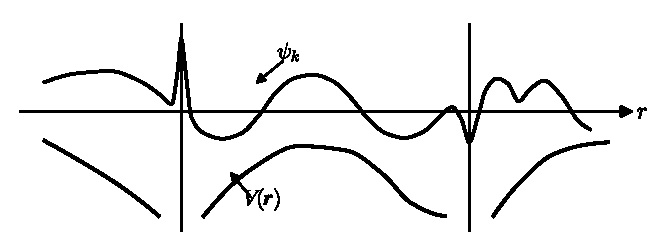
\includegraphics[width=7cm]{fig8-1.pdf}\\{\small 图 8.1\quad 布洛赫函数在离子实区的振荡特征}
\end{minipage}
\end{center}

表8.1\quad 由 $k=0$ W-S 元胞法波函数所算出的 Li 的 $a(\boldsymbol{K})$

\begin{center}\small
\begin{tabular}{ccc}
\hline
$|\boldsymbol{K}|$（以 $k_{\mathrm{F}}=0.589$ 原子单位量度） & 长度为 $|\boldsymbol{K}|$ 的倒格点个数 & $(N\Omega)^{1/2}a(\boldsymbol{K})$\\
\hline
0 & 1 & $-0.948$\\
1.353 & 12 & $+0.062$\\
1.914 & 6 & $+0.041$\\
2.344 & 24 & $+0.029$\\
2.706 & 12 & $+0.021$\\
3.026 & 24 & $+0.016$\\
3.315 & 8 & $+0.013$\\
3.580 & 48 & $+0.010$\\
3.828 & 6 & $+0.008$\\
4.060 & 36 & $+0.007$\\
4.279 & 24 & $+0.006$\\
4.488 & 24 & $+0.005$\\
$|\boldsymbol{K}|$（以 $k_{\mathrm{F}}=0.589$ 原子单位量度） & 长度为 $|\boldsymbol{K}|$ 的倒格点个数 & $(N\Omega)^{1/2}a(\boldsymbol{K})$\\
4.688 & 24 & $+0.004$\\
4.879 & 72 & $+0.004$\\
5.241 & 48 & $+0.003$\\
5.413 & 12 & $+0.003$\\
5.580 & 48 & $+0.002$\\
5.742 & 30 & $+0.002$\\
\hline
\end{tabular}
\end{center}

\section{正交化平面波法}

赫令（C.Herring）\textsuperscript{[2]}提出一种克服平面波展开收敛差的办法.首先将固体能带分为两类：壳层电子的能带和价带及导带，价带指的是最高的一个被占据能带，导带则代表最低的一个空（或半空）的能带.众所周知，费密面必然位于导带与价带附近，由于固体的特性主要由费密面附近电子的运动决定，所以人们感兴趣的是导带及价带结构.对于较低的壳层电子能带，一般都被填满，而且多半是窄能带，可以用紧束缚波函数表示为
\begin{equation}
  |\psi_{\mathrm{c}}\rangle=\frac{1}{\sqrt{N}}\sum_{\boldsymbol{l}}\mathrm{e}^{\mathrm{i}\boldsymbol{k}\cdot\boldsymbol{l}}|\phi_{\mathrm{c}}\rangle
\end{equation}
其中 $|\phi_{\mathrm{c}}\rangle$ 代表位于格点 $\boldsymbol{l}$ 上的原子波函数 $\phi_{\mathrm{c}}(\boldsymbol{r}-\boldsymbol{l})$，并假定为已知，它们满足本征方程
\begin{equation}
  H|\psi_{\mathrm{c}}\rangle=E_{\mathrm{c}}|\psi_{\mathrm{c}}\rangle
\end{equation}
当离子实体积很小，以致相邻格点的离子实波函数之间重叠可忽略时，$|\psi_{\mathrm{c}}\rangle$ 的表示式(8.2.1)就代表已归一化的壳层电子能带波函数，并满足条件
\begin{equation}
  \langle\psi_{\mathrm{c}'}|\psi_{\mathrm{c}}\rangle=\delta_{\mathrm{cc}'}
\end{equation}
其中 $\mathrm{c}$ 代表壳层态量子数，如1s，2p，….除贵金属与过渡金属外，对于单价及多价金属上述条件是合理的.例如，在铅（Pb）中 $1\mathrm{s}^{2}\cdots5\mathrm{s}^{2}5\mathrm{p}^{6}\mathrm{d}^{10}$ 代表离子实，$6\mathrm{s}^{2}6\mathrm{p}^{2}$ 为价电子态，其离子实的尺寸只有原子的一半，这时离子实只占总原子体积的1/8，故式(8.2.3)为合理的近似.

赫令注意到，对于固体中运动的电子，元胞中的离子实内区与离子实外区是两种性质上不同的区域.当导带或价带电子处于在离子实区以外时，仅受到弱势场作用，波函数在空间平滑变化，这时 $\psi_{\boldsymbol{k}}(\boldsymbol{r})$ 像平面波.在离子实区以内，由于有很强的局域势场作用，电子波函数表现出原子波函数的急剧振荡特征.因此最好采用平面波 $|\boldsymbol{k}+\boldsymbol{K}\rangle$ 与壳层能带波函数 $|\psi_{\mathrm{c}}\rangle$ 的某种线性组合来描述布洛赫函数，这样做才能兼顾两方面特征，应当说是更为切合实际情况的物理图像.
\begin{equation}
  |\psi_{\boldsymbol{k}}\rangle=\sum_{\boldsymbol{K}}\alpha(\boldsymbol{k}+\boldsymbol{K})|\boldsymbol{k}+\boldsymbol{K}\rangle+\sum_{\mathrm{c}}\beta_{\mathrm{c}}|\psi_{\mathrm{c}}\rangle
\end{equation}
系数 $\beta_{\mathrm{c}}$ 则由下面的正交化条件决定
\begin{equation}
  \langle\psi_{\mathrm{c}}|\psi_{\boldsymbol{k}}\rangle=0
\end{equation}
因为价带或导带的布洛赫函数与壳层能带波函数 $|\psi_{\mathrm{c}}\rangle$ 都是同一薛定谔方程不同本征值的解，它们理所当然的应当彼此正交.这个条件给出
\begin{equation}
  \beta_{\mathrm{c}}=-\sum_{\boldsymbol{K}}\alpha(\boldsymbol{k}+\boldsymbol{K})\langle\phi_{\mathrm{c}}|\boldsymbol{k}+\boldsymbol{K}\rangle
\end{equation}
由此求得导带及价带布洛赫函数的表示式：
\begin{equation}
\begin{aligned}
  |\phi_{\boldsymbol{k}}\rangle
  &=\sum_{\boldsymbol{K}}\alpha(\boldsymbol{k}+\boldsymbol{K})\Bigl[|\boldsymbol{k}+\boldsymbol{K}\rangle-\sum_{\mathrm{c}}|\phi_{\mathrm{c}}\rangle\langle\phi_{\mathrm{c}}|\boldsymbol{k}+\boldsymbol{K}\rangle\Bigr]\\
  &=\sum_{\boldsymbol{K}}\alpha(\boldsymbol{k}+\boldsymbol{K})|\mathrm{OPW}_{\boldsymbol{k}+\boldsymbol{K}}\rangle
\end{aligned}
\end{equation}
其中
\begin{equation}
  |\mathrm{OPW}_{\boldsymbol{k}}\rangle\equiv|\boldsymbol{k}\rangle-\sum_{\mathrm{c}}|\psi_{\mathrm{c}}\rangle\langle\psi_{\mathrm{c}}|\boldsymbol{k}\rangle
\end{equation}
称为正交化平面波（以下简称OPW），它是波矢为 $\boldsymbol{k}$ 的简单平面波与所有壳层能带的紧束缚波函数的特殊线性组合.组合结果必须与每一壳层能带波函数正交，即
\begin{equation}
  \langle\psi_{\mathrm{c}}|\mathrm{OPW}_{\boldsymbol{k}+\boldsymbol{K}}\rangle
  =\langle\psi_{\mathrm{c}}|\boldsymbol{k}+\boldsymbol{K}\rangle\Bigl(1-\sum_{\mathrm{c}'}\langle\psi_{\mathrm{c}}|\psi_{\mathrm{c}'}\rangle\Bigr)=0
\end{equation}
导（或价）带的布洛赫函数则是按正交化平面波 $|\mathrm{OPW}\rangle$ 展开表示的“傅里叶级数”，如式(8.2.7).将式(8.2.7)代入式(8.1.1)得
\begin{equation}
\begin{aligned}
  &(T+V-E)|\phi_{\boldsymbol{k}}\rangle\\
  &\quad=\sum_{\boldsymbol{K}}\alpha(\boldsymbol{k}+\boldsymbol{K})\bigl[(T+V-E)|\boldsymbol{k}+\boldsymbol{K}\rangle\\
  &\qquad-(T+V-E)\sum_{\mathrm{c}}|\phi_{\mathrm{c}}\rangle\langle\phi_{\mathrm{c}}|\boldsymbol{k}+\boldsymbol{K}\rangle\bigr]\\
  &\quad=0
\end{aligned}
\end{equation}
由于
\begin{equation}
  (T+V)|\psi_{\mathrm{c}}\rangle=E_{\mathrm{c}}|\psi_{\mathrm{c}}\rangle
\end{equation}
式(8.2.10)可写成
\begin{equation}
\begin{aligned}
  \sum_{\boldsymbol{K}}\alpha(\boldsymbol{k}+\boldsymbol{K})\biggl\{\Bigl[\frac{\hbar^{2}(\boldsymbol{k}+\boldsymbol{K})^{2}}{2m}-E\Bigr]|\boldsymbol{k}+\boldsymbol{K}\rangle+V|\boldsymbol{k}+\boldsymbol{K}\rangle\\
  +\sum_{\mathrm{c}}(E-E_{\mathrm{c}})|\phi_{\mathrm{c}}\rangle\langle\phi_{\mathrm{c}}|\boldsymbol{k}+\boldsymbol{K}\rangle\biggr\}=0
\end{aligned}
\end{equation}
将 $\langle\boldsymbol{k}+\boldsymbol{K}'|$ 作用于上式，求得 $\alpha$ 的线性方程组
\begin{equation}
\begin{aligned}
  \sum_{\boldsymbol{K}}\alpha(\boldsymbol{k}+\boldsymbol{K})\biggl\{\Bigl[\frac{\hbar^{2}(\boldsymbol{k}+\boldsymbol{K})^{2}}{2m}-E\Bigr]\delta_{\boldsymbol{K}\boldsymbol{K}'}\\
  +\langle\boldsymbol{k}+\boldsymbol{K}'|U|\boldsymbol{k}+\boldsymbol{K}\rangle\biggr\}=0
\end{aligned}
\end{equation}
其中矩阵元定义为
\begin{equation}
\begin{aligned}
  &\langle\boldsymbol{k}+\boldsymbol{K}'|U|\boldsymbol{k}+\boldsymbol{K}\rangle\\
  &\quad=\langle\boldsymbol{k}+\boldsymbol{K}'|V|\boldsymbol{k}+\boldsymbol{K}\rangle\\
  &\qquad+\sum_{\mathrm{c}}(E-E_{\mathrm{c}})\langle\boldsymbol{k}+\boldsymbol{K}'|\psi_{\mathrm{c}}\rangle\langle\psi_{\mathrm{c}}|\boldsymbol{k}+\boldsymbol{K}\rangle
\end{aligned}
\end{equation}
而决定能量本征值的久期方程为
\begin{equation}
\begin{aligned}
  \mathrm{det}\,\Bigl\|\Bigl[\frac{\hbar^{2}}{2m}(\boldsymbol{k}+\boldsymbol{K})^{2}-E\Bigr]\delta_{\boldsymbol{K}\boldsymbol{K}'}\\
  +\langle\boldsymbol{k}+\boldsymbol{K}'|U|\boldsymbol{k}+\boldsymbol{K}\rangle\Bigr\|=0
\end{aligned}
\end{equation}
这个行列式原则上也是无穷维的，但在实际应用中往往只需取少数几项就足够了.例如，对于锂（Li）只取展开式(8.2.7)中的一项（即一个正交化平面波），就能得出适用于价带的合理结果\textsuperscript{[3]}.应用为数不多的OPW作展开计算半导体锗 $(\mathrm{Ge})$\textsuperscript{[4]} 和硅 $(\mathrm{Si})$\textsuperscript{[5]} 的能带也取得了成功.比较图8.2中(a)平面波、(b)离子实波和(c)正交化平面波，可以看出一个OPW本身就包括了电子在离子实区的多次振荡特征.所以，一个OPW已经十分逼近真实波函数了，若进一步用OPW作展开表示 $\psi_{\boldsymbol{k}}$，其收敛必然比 $\psi_{\boldsymbol{k}}$ 平面波展开快得多.因此，OPW法是描述价带和导带电子波函数的好表象，是定量计算能带的一种重要方法.

关于OPW方法收敛性快的问题，还可以通过一个具体例子加以说明：例如计算金属锂的OPW矩阵元时，可取Li原子的1s态：
\begin{equation*}
\begin{aligned}
  &\phi_{\mathrm{c}}=\phi_{1\mathrm{s}}=\frac{\lambda^{3/2}}{\sqrt{\pi}}\exp(-\lambda r)
  \qquad\left(\lambda=2.37\,[\mathrm{a.u.}]^{-1}\right)\\
  &E_{\mathrm{c}}=E_{1\mathrm{s}}=-3.765\ [\mathrm{Ry}],\qquad V(\boldsymbol{r})=-\frac{e^{2}}{r}
\end{aligned}
\end{equation*}
则式(8.2.14)在 $\boldsymbol{K}'=\boldsymbol{0}$ 与 $E\approx\hbar^{2}k^{2}/2m$ 时可写为

\begin{center}
\begin{minipage}{7.5cm}
\centering
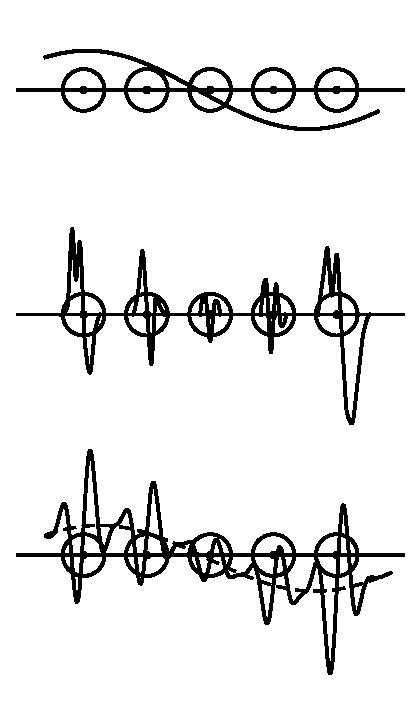
\includegraphics[width=7.5cm]{fig8-2.pdf}\\[0.3em]
{\small (a) 平面波\qquad\qquad (b) 离子实波\qquad\qquad (c) 正交化平面波}\\[0.2em]
{\small 图 8.2}
\end{minipage}
\end{center}

\begin{equation}
\begin{aligned}
  &\langle\boldsymbol{k}|U|\boldsymbol{k}+\boldsymbol{K}\rangle\\
  &\quad=\langle\boldsymbol{k}|V|\boldsymbol{k}+\boldsymbol{K}\rangle
  +\Bigl(\frac{\hbar^{2}k^{2}}{2m}+|E_{1\mathrm{s}}|\Bigr)
  \langle\boldsymbol{k}|\phi_{1\mathrm{s}}\rangle\langle\phi_{1\mathrm{s}}|\boldsymbol{k}+\boldsymbol{K}\rangle
\end{aligned}
\end{equation}
其中
\begin{equation*}
\begin{aligned}
  \langle\boldsymbol{k}|V|\boldsymbol{k}+\boldsymbol{K}\rangle
  &=\frac{1}{N\Omega}\int\mathrm{e}^{-\mathrm{i}\boldsymbol{k}\cdot\boldsymbol{r}}\Bigl(-\frac{e^{2}}{r}\Bigr)\mathrm{e}^{\mathrm{i}(\boldsymbol{k}+\boldsymbol{K})\cdot\boldsymbol{r}}\mathrm{d}\boldsymbol{r}\\
  &=\frac{1}{N\Omega}\int\Bigl(-\frac{e^{2}}{r}\Bigr)\mathrm{e}^{\mathrm{i}\boldsymbol{K}\cdot\boldsymbol{r}}\mathrm{d}\boldsymbol{r}
  =-\frac{4\pi e^{2}}{\Omega K^{2}}\\
  \langle\boldsymbol{k}|\psi_{1\mathrm{s}}\rangle
  &=\frac{1}{(N\Omega)^{1/2}}\int\mathrm{e}^{-\mathrm{i}\boldsymbol{k}\cdot\boldsymbol{r}}\psi_{1\mathrm{s}}(\boldsymbol{r})\mathrm{d}\boldsymbol{r}\\
  &=\frac{8\sqrt{\pi}}{(N\Omega)^{1/2}\lambda^{3/2}}\Bigl(1+\frac{k^{2}}{\lambda^{2}}\Bigr)^{-2}
\end{aligned}
\end{equation*}
求得OPW矩阵元
\begin{equation}
\begin{aligned}
  \langle\boldsymbol{k}|U|\boldsymbol{k}+\boldsymbol{K}\rangle
  &=-\frac{4\pi e^{2}}{N\Omega K^{2}}
  +\frac{64\pi}{N\Omega\lambda^{3}}
  \Bigl[\Bigl(1+\frac{k^{2}}{\lambda^{2}}\Bigr)
  \Bigl(1+\frac{|\boldsymbol{k}+\boldsymbol{K}|^{2}}{\lambda^{2}}\Bigr)\Bigr]^{-2}\times\\
  &\qquad\Bigl(\frac{\hbar^{2}k^{2}}{2m}+|E_{1\mathrm{s}}|\Bigr)
\end{aligned}
\end{equation}
上式右边第一项代表真实势 $V(\boldsymbol{r})$ 的矩阵元，第二项来源于正交化手续，它是一个正量，将对第一项起抵消作用，使 $\langle\boldsymbol{k}|U|\boldsymbol{k}+\boldsymbol{K}\rangle$ 成为比真实势弱的有效势矩阵元，从而有可能用低阶微扰处理OPW计算，自然其收敛性会比平面波法好.

\section{赝势方法}

已经看到，OPW方法中的正交化项起抵消势能的作用，并因此给出一个比真实势弱得多的有效势，试问能否在这种抵消作用的基础上发展一种计算导带和价带的新方案？赝势方法就是这样被提出来的.

\subsection*{1. OPW赝势}

将布洛赫函数的OPW展开式(8.2.7)写为
\begin{equation}
  |\psi_{\boldsymbol{k}}\rangle=|\chi_{\boldsymbol{k}}\rangle-\sum_{\mathrm{c}}|\psi_{\mathrm{c}}\rangle\langle\psi_{\mathrm{c}}|\chi_{\boldsymbol{k}}\rangle
\end{equation}
这里引进一个新函数
\begin{equation}
  |\chi_{\boldsymbol{k}}\rangle=\sum_{\boldsymbol{K}}\alpha(\boldsymbol{k}+\boldsymbol{K})|\boldsymbol{k}+\boldsymbol{K}\rangle
\end{equation}
并设其中的展开系数与OPW展开式(8.2.7)中的 $\alpha(\boldsymbol{k}+\boldsymbol{K})$ 相同.为说明这样组合的简单平面波的特征，先讨论 $|\chi_{\boldsymbol{k}}\rangle$ 满足什么方程.

将 $|\psi_{\boldsymbol{k}}\rangle$ 代入薛定谔方程
\begin{equation}
  H|\psi_{\boldsymbol{k}}\rangle=E_{k}|\psi_{\boldsymbol{k}}\rangle
\end{equation}
得
\begin{equation}
  H|\chi_{\boldsymbol{k}}\rangle-\sum_{\mathrm{c}}\langle\psi_{\mathrm{c}}|\chi_{\boldsymbol{k}}\rangle H|\psi_{\mathrm{c}}\rangle
  =E_{k}|\chi_{\boldsymbol{k}}\rangle-E_{k}\sum_{\mathrm{c}}\langle\psi_{\mathrm{c}}|\chi_{\boldsymbol{k}}\rangle|\psi_{\mathrm{c}}\rangle
\end{equation}
利用
\begin{equation}
  H|\psi_{\mathrm{c}}\rangle=E_{\mathrm{c}}|\psi_{\mathrm{c}}\rangle
\end{equation}
可求得 $|\chi_{\boldsymbol{k}}\rangle$ 的方程式
\begin{equation}
  H|\chi_{\boldsymbol{k}}\rangle+\sum_{\mathrm{c}}(E_{k}-E_{\mathrm{c}})|\psi_{\mathrm{c}}\rangle\langle\psi_{\mathrm{c}}|\chi_{\boldsymbol{k}}\rangle=E_{k}|\chi_{\boldsymbol{k}}\rangle
\end{equation}
再利用式(8.1.1)写为
\begin{equation}
  (T+U)|\chi_{\boldsymbol{k}}\rangle=E_{k}|\chi_{\boldsymbol{k}}\rangle
\end{equation}
其中
\begin{equation}
  U|\chi_{\boldsymbol{k}}\rangle=V|\chi_{\boldsymbol{k}}\rangle
  +\sum_{\mathrm{c}}(E_{k}-E_{\mathrm{c}})|\psi_{\mathrm{c}}\rangle\langle\psi_{\mathrm{c}}|\chi_{\boldsymbol{k}}\rangle
\end{equation}
$U=V+\sum_{\mathrm{c}}(E_{k}-E_{\mathrm{c}})|\psi_{\mathrm{c}}\rangle\langle\psi_{\mathrm{c}}|$ 称为赝势，而 $|\chi_{\boldsymbol{k}}\rangle$ 是在赝势作用下运动的电子波函数，人们称之为赝波函数.比较式(8.3.3)和(8.3.7)可知，赝波函数 $|\chi_{\boldsymbol{k}}\rangle$ 与布洛赫函数 $|\psi_{\boldsymbol{k}}\rangle$ 具有完全相同的能量本征值 $E_{k}$，这是赝势方法的重要特点.现在分析赝势的大小，注意到 $E_{k}$ 为导（或价）带中电子能量，显然它应当大于壳层态中的电子能量 $E_{\mathrm{c}}$，使 $U$ 中第二项的贡献为正.所以，赝势中正交化所带来的是一个排斥势，它与真实的吸引势有相消趋势.从物理上看，要求价电子态与被填满的离子实轨道态正交相当于泡利不相容原理，而正交性要求必然使价电子波函数在离子实区引进振荡\footnote{因为离子实中壳层电子波函数是振荡的，价电子波函数也必须在离子实区内振荡，否则两者不能正交.}.这种急剧振荡又将使价电子产生高平均动能，并对离子实区的强吸引势起抵消作用，因此价电子实际上只受到弱的净势作用，相当于一个微扰势，这就是赝势.当我们用赝势取代真实势解薛定谔方程时，相应的赝波函数也就没有复杂的振荡特征了.

综上所述，从OPW出发，我们可以找到一个赝波动方程(8.3.7)，它与严格布洛赫函数的能量本征值相同，但赝势和赝波函数相对于真实势和严格波函数都是被平滑化了的，所以组合少数平面波就足以描述赝波函数的展式(8.3.2)了.因此，计算能带时不必先求布洛赫函数，可直接从式(8.3.8)出发，先计算赝势，然后用赝波动方程(8.3.7)求解平滑函数所对应的能量 $E_{k}$ 值，这就是建立在OPW基础上的赝势方法，它原则上等同于作OPW计算，因为在这里要求式(8.2.7)与(8.3.2)的展开系数 $\alpha(\boldsymbol{k}+\boldsymbol{K})$ 相同.

\subsection*{2. 赝势法的非唯一性特征}

赝势法的优点不仅如此.现在我们将超出OPW的范围，更一般地讨论赝势法.

一般赝势法原则上也是利用价带或导带电子波函数与离子实电子波函数正交的事实.从布洛赫函数的薛定谔方程出发
\begin{equation*}
  (T+V)|\psi_{\boldsymbol{k}}\rangle=E_{k}|\psi_{\boldsymbol{k}}\rangle
\end{equation*}
利用正交条件 $\langle\psi_{\mathrm{c}}|\psi_{\boldsymbol{k}}\rangle=0$，得到形式上与式(8.3.1)相同的表示式
\begin{equation}
  |\psi_{\boldsymbol{k}}\rangle=|\chi_{\boldsymbol{k}}\rangle-\sum_{\mathrm{c}}|\psi_{\mathrm{c}}\rangle\langle\psi_{\mathrm{c}}|\chi_{\boldsymbol{k}}\rangle
\end{equation}
这里 $|\chi_{\boldsymbol{k}}\rangle$ 是一般的赝波函数.它满足赝波动方程（赝势方程）
\begin{equation}
  (T+U)|\chi_{\boldsymbol{k}}\rangle=E_{k}|\chi_{\boldsymbol{k}}\rangle
\end{equation}
其中
\begin{equation}
  U|\chi_{\boldsymbol{k}}\rangle=V|\chi_{\boldsymbol{k}}\rangle
  +\sum_{\mathrm{c}}(E_{k}-E_{\mathrm{c}})|\phi_{\mathrm{c}}\rangle\langle\phi_{\mathrm{c}}|\chi_{\boldsymbol{k}}\rangle
\end{equation}
试问 $|\chi_{\boldsymbol{k}}\rangle$ 有何特性？不难看出，若将壳层波函数的任意线性组合附加于 $|\chi_{\boldsymbol{k}}\rangle$，则新赝波函数
\begin{equation}
  |\chi'_{\boldsymbol{k}}\rangle=|\chi_{\boldsymbol{k}}\rangle+\sum_{\mathrm{c}'}\gamma_{\mathrm{c}'}|\psi_{\mathrm{c}'}\rangle
\end{equation}
满足同样的赝波动方程：
\begin{equation}
\begin{aligned}
  (T+U)|\chi'_{\boldsymbol{k}}\rangle
  &=(T+U)|\chi_{\boldsymbol{k}}\rangle+(T+U)\sum_{\mathrm{c}'}\gamma_{\mathrm{c}'}|\psi_{\mathrm{c}'}\rangle\\
  &=E_{k}|\chi_{\boldsymbol{k}}\rangle+H\sum_{\mathrm{c}'}\gamma_{\mathrm{c}'}|\psi_{\mathrm{c}'}\rangle+(U-V)\sum_{\mathrm{c}'}\gamma_{\mathrm{c}'}|\psi_{\mathrm{c}'}\rangle\\
  &=E_{k}|\chi_{\boldsymbol{k}}\rangle+\sum_{\mathrm{c}'}\gamma_{\mathrm{c}'}E_{\mathrm{c}'}|\psi_{\mathrm{c}'}\rangle
  +\sum_{\mathrm{c}',\mathrm{c}}\gamma_{\mathrm{c}'}(E_{k}-E_{\mathrm{c}})|\psi_{\mathrm{c}}\rangle\langle\psi_{\mathrm{c}}|\psi_{\mathrm{c}'}\rangle\\
  &=E_{k}\Bigl(|\chi_{\boldsymbol{k}}\rangle+\sum_{\mathrm{c}'}\gamma_{\mathrm{c}'}|\psi_{\mathrm{c}'}\rangle\Bigr)\\
  &=E_{k}|\chi'_{\boldsymbol{k}}\rangle
\end{aligned}
\end{equation}
以上结果说明：当 $|\chi_{\boldsymbol{k}}\rangle$ 是赝势方程的解时，$|\chi'_{\boldsymbol{k}}\rangle$ 也是此方程同一本征值 $E_{k}$ 的解，这就是赝波动方程解的非唯一性特征.在推导式(8.3.13)时，利用了 $\langle\psi_{\mathrm{c}}|\psi_{\mathrm{c}'}\rangle=\delta_{\mathrm{cc}'}$.

与此相应，赝势 $U$ 的选取也是非唯一的.1962年奥斯丁（Austin）等人\textsuperscript{[6]}指出，利用正交条件 $\langle\psi_{\boldsymbol{k}}|\psi_{\mathrm{c}}\rangle=0$，由式(8.3.11)可求出赝势条件
\begin{equation}
  \langle\psi_{\boldsymbol{k}}|(U-V)|\chi_{\boldsymbol{k}}\rangle=0
\end{equation}
满足这个条件的一般赝势为
\begin{equation}
  U|\chi_{\boldsymbol{k}}\rangle=V|\chi_{\boldsymbol{k}}\rangle+\sum_{\mathrm{c}}|\psi_{\mathrm{c}}\rangle\langle\psi_{\mathrm{c}}|F|\chi_{\boldsymbol{k}}\rangle
\end{equation}
其中 $F$ 为任意算子，因为 $\langle\psi_{\boldsymbol{k}}|\psi_{\mathrm{c}}\rangle=0$ 可保证以上赝势 $U$ 仍满足式(8.3.14)，按式(8.3.15)决定的 $U$ 称为广义赝势.在式(8.3.15)中若取 $F=0$，将回到布洛赫波函数的薛定谔方程，若取 $F=E_{k}-H$，则是OPW赝势方程(8.3.8).由此可知，赝势的选择也不是唯一的.对于导带或价带电子，凡满足式(8.3.14)的任何赝势都给出相同的能量本征值 $E_{k}$.

非唯一性是赝势法的固有特性，利用它可选定最佳赝势使赝波函数尽可能平滑.在具体计算时，可利用变分技巧，要求赝势尽可能小，从而决定 $\langle\psi_{\mathrm{c}}|F|\chi_{\boldsymbol{k}}\rangle$，或者从赝波函数尽可能是空间缓慢变化的要求确定系数 $\gamma_{\mathrm{c}'}$，这两种要求大体上是等效的.按此选定的赝波函数可近似由少数平面波叠加构成，这是赝势方法的核心.

总之，赝势的引入将 $H=T+V$ 换成 $H_{\mathrm{ps}}=T+U$，可以求出与 $H$ 一样的本征值 $E_{k}$，但其波函数 $\chi_{k}$ 已是空间的缓变函数，可以用平面波作为良好近似，并将使能谱的求解大为简化.

\subsection*{3. 赝势计算方案}

若将 $|\chi_{\boldsymbol{k}}\rangle$ 展开为平面波，可求得与§1中相同的久期方程，只不过真实势 $V$ 的矩阵元 $\langle\boldsymbol{k}'+\boldsymbol{K}'|V|\boldsymbol{k}+\boldsymbol{K}\rangle$ 换成了赝势 $U$ 的矩阵元.困难在于 $U$ 是非定域势（即积分算子），假如近似用一个定域的赝势 $U(\boldsymbol{r})$ 来描述，则
\begin{equation}
  \langle\boldsymbol{k}+\boldsymbol{K}'|U|\boldsymbol{k}+\boldsymbol{K}\rangle
  =\frac{1}{N\Omega}\int U(\boldsymbol{r})\mathrm{e}^{-\mathrm{i}\boldsymbol{q}\cdot\boldsymbol{r}}\mathrm{d}\boldsymbol{r}
  \qquad(\boldsymbol{q}=\boldsymbol{K}'-\boldsymbol{K})
\end{equation}
将 $U(\boldsymbol{r})$ 用各离子赝势之和表示，对于每个元胞中含多个原子的复式晶格情况，得到
\begin{equation}
  U(\boldsymbol{r})=\sum_{\alpha,\,\boldsymbol{l}}v_{\alpha}(\boldsymbol{r}-\boldsymbol{l}-\boldsymbol{R}_{\alpha})
\end{equation}
其中 $v_{\alpha}$ 代表元胞中第 $\alpha$ 个离子的势能，$\boldsymbol{R}_{\alpha}$ 为其在元胞中的位置矢.$U(\boldsymbol{r})$ 的傅里叶分量为
\begin{equation}
\begin{aligned}
  U(\boldsymbol{q})&=\langle\boldsymbol{k}+\boldsymbol{K}'|U|\boldsymbol{k}+\boldsymbol{K}\rangle\\
  &=\frac{1}{N\Omega}\sum_{\alpha,\,\boldsymbol{l}}\int v_{\alpha}(\boldsymbol{r}-\boldsymbol{l}-\boldsymbol{R}_{\alpha})\mathrm{e}^{-\mathrm{i}\boldsymbol{q}\cdot\boldsymbol{r}}\mathrm{d}\boldsymbol{r}\\
  &=\frac{1}{\Omega}\sum_{\alpha}\mathrm{e}^{-\mathrm{i}\boldsymbol{q}\cdot\boldsymbol{R}_{\alpha}}\int v_{\alpha}(\boldsymbol{r})\mathrm{e}^{-\mathrm{i}\boldsymbol{q}\cdot\boldsymbol{r}}\mathrm{d}\boldsymbol{r}\\
  &=\sum_{\alpha}\mathrm{e}^{-\mathrm{i}\boldsymbol{q}\cdot\boldsymbol{R}_{\alpha}}I_{\alpha}
\end{aligned}
\end{equation}
其中
\begin{equation}
  I_{\alpha}\equiv\frac{1}{\Omega}\int v_{\alpha}(\boldsymbol{r})\mathrm{e}^{-\mathrm{i}\boldsymbol{q}\cdot\boldsymbol{r}}\mathrm{d}\boldsymbol{r}
\end{equation}
叫形状因子.对于全同原子组成的晶体，$I_{\alpha}$ 与 $\alpha$ 无关，这时
\begin{equation}
  U(\boldsymbol{q})=I\sum_{\alpha}\mathrm{e}^{-\mathrm{i}\boldsymbol{q}\cdot\boldsymbol{R}_{\alpha}}\equiv IS(\boldsymbol{q})
\end{equation}
$S(\boldsymbol{q})$ 称为结构因子.当所选赝势足够平滑时，$U(\boldsymbol{q})$ 中只有小 $\boldsymbol{q}$ 值的傅里叶分量是重要的，这时久期行列式的维数变得很小，只要已知形状因子 $I_{\alpha}$，能带结构就不难算出.在定量计算时，$I_{\alpha}$ 由实验值确定.

还可以利用赝势的非唯一性，把离子实区的赝势取得尽量简单，并引进一组可调参量，最后由匹配条件决定这些参量，以保证在离子实区以外 $|\chi_{\boldsymbol{k}}\rangle$ 与 $|\psi_{\boldsymbol{k}}\rangle$ 一致.例如，海因（Heine）等人\textsuperscript{[7]}将离子的真实势在离子实区用一个方阱模型代替（如图8.3所示）.
\begin{equation}
  U_{\mathrm{M}}=\begin{cases}
    -A_{l} & (\boldsymbol{r}\leqslant\boldsymbol{a}_{\mathrm{M}})\\[0.2em]
    -\dfrac{Ze^{2}}{r} & (\boldsymbol{r}>\boldsymbol{a}_{\mathrm{M}})
  \end{cases}
\end{equation}
其中 $Z$ 为化学价，$A_{l}$ 为阱深，它与壳层态量子数 $l$ 有关.调节参数 $A_{l}$ 与 $a_{\mathrm{M}}$，可使模型赝势的波动方程解与观测的自由原子光谱项一致，这种办法很成功地用于原子问题，避免了解自洽方程的麻烦.当用于固体时，设在 $r\leqslant a_{\mathrm{M}}$ 时赝势为 $-A(E)$，在最简单情况下可令它等于零，而可调参量 $a_{\mathrm{M}}$ 则由 $r=a_{\mathrm{M}}$ 处赝波函数与布洛赫函数相等条件决定.图8.4对晶体的真实势和赝势以及布洛赫函数和赝波函数作了比较.

\begin{center}
\begin{minipage}{6.5cm}
\centering
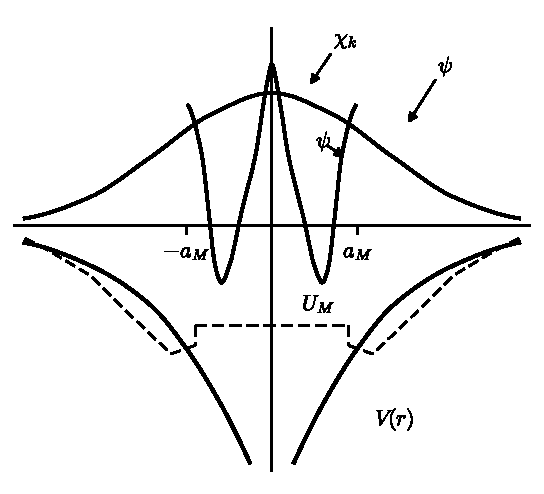
\includegraphics[width=6.5cm]{fig8-3.pdf}\\{\small 图 8.3\quad 用于离子的模型赝势}
\end{minipage}
\end{center}

\begin{center}
\begin{minipage}{8cm}
\centering
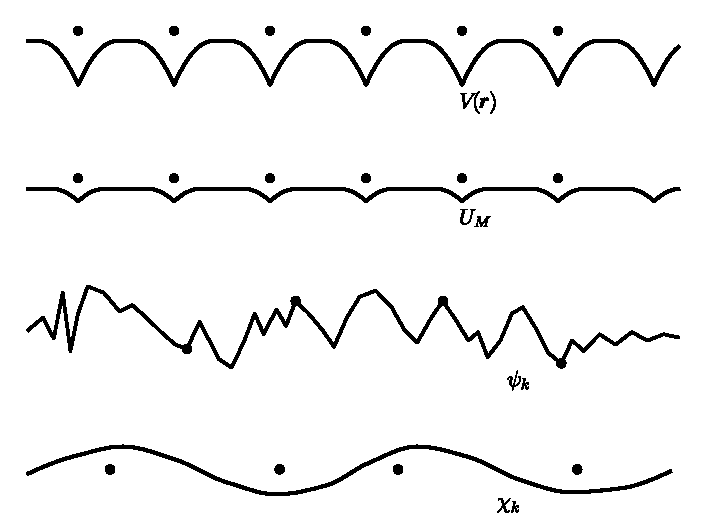
\includegraphics[width=8cm]{fig8-4.pdf}\\[0.3em]
{\small (a) 晶体势 $V(\boldsymbol{r})$\qquad\qquad (b) 赝势 $U_{\mathrm{M}}$}\\[0.2em]
{\small (c) 布洛赫函数 $\psi_{\boldsymbol{k}}$\qquad\qquad (d) 赝波函数 $\chi_{\boldsymbol{k}}$}\\[0.2em]
{\small 图 8.4\quad 晶体中模型赝势的示意图}
\end{minipage}
\end{center}
\section{近自由电子方法的赝势证明}

引入赝势的另一重要成就是：证明了近自由电子方法适用于离子实半径小的金属能带计算，其证明如下.

鉴于赝波函数的非唯一性，我们希望能找到一个平滑的 $\chi_{\boldsymbol{k}}$，显然其选择条件要求下列量
\begin{equation}
  \frac{\int|\nabla\chi_{\boldsymbol{k}}|^{2}\,\mathrm{d}\tau}{\int|\chi_{\boldsymbol{k}}|^{2}\,\mathrm{d}\tau}
\end{equation}
为极小，此要求等效于动能极小条件，因为
\begin{equation}
\begin{aligned}
  \int|\nabla\chi_{\boldsymbol{k}}|^{2}\,\mathrm{d}\tau
  &=\int\nabla\chi_{\boldsymbol{k}}^{*}\cdot\nabla\chi_{\boldsymbol{k}}\,\mathrm{d}\tau\\
  &=\int_{S}(\chi_{\boldsymbol{k}}^{*}\nabla\chi_{\boldsymbol{k}})\cdot\mathrm{d}\boldsymbol{S}
  -\int\chi_{\boldsymbol{k}}^{*}\nabla^{2}\chi_{\boldsymbol{k}}\,\mathrm{d}\tau
\end{aligned}
\end{equation}
由于周期性边界条件，上式右边的面积分项为零，而第二项正比于动能.所以，可利用动能极小条件选择最佳的 $\chi_{\boldsymbol{k}}$，设
\begin{equation}
  \overline{T}=\frac{\langle\chi_{\boldsymbol{k}}|T|\chi_{\boldsymbol{k}}\rangle}{\langle\chi_{\boldsymbol{k}}|\chi_{\boldsymbol{k}}\rangle}
\end{equation}
则其变分方程为
\begin{equation}
  \langle\delta\chi|T|\chi_{\boldsymbol{k}}\rangle-\overline{T}\langle\delta\chi|\chi_{\boldsymbol{k}}\rangle=0
\end{equation}
按照赝波函数的非唯一性，取 $|\delta\chi\rangle=\sum_{\mathrm{c}}\gamma_{\mathrm{c}}|\psi_{\mathrm{c}}\rangle$，得到
\begin{equation}
  \langle\psi_{\mathrm{c}}|T|\chi_{\boldsymbol{k}}\rangle-\overline{T}\langle\psi_{\mathrm{c}}|\chi_{\boldsymbol{k}}\rangle=0
\end{equation}
由此求得
\begin{equation}
  \langle\psi_{\mathrm{c}}|(E_{k}-T)|\chi_{\boldsymbol{k}}\rangle
  =(E_{k}-\overline{T})\langle\psi_{\mathrm{c}}|\chi_{\boldsymbol{k}}\rangle
\end{equation}
将上式代入广义赝势的表示式(8.3.15)并取 $F=E_{k}-H$
\begin{equation}
\begin{aligned}
  U|\chi_{\boldsymbol{k}}\rangle
  &=V|\chi_{\boldsymbol{k}}\rangle+\sum_{\mathrm{c}}|\psi_{\mathrm{c}}\rangle\langle\psi_{\mathrm{c}}|F|\chi_{\boldsymbol{k}}\rangle\\
  &=V|\chi_{\boldsymbol{k}}\rangle+\sum_{\mathrm{c}}|\psi_{\mathrm{c}}\rangle\langle\psi_{\mathrm{c}}|(E_{k}-H)|\chi_{\boldsymbol{k}}\rangle\\
  &=V|\chi_{\boldsymbol{k}}\rangle+\sum_{\mathrm{c}}|\psi_{\mathrm{c}}\rangle\langle\psi_{\mathrm{c}}|(E_{k}-T)|\chi_{\boldsymbol{k}}\rangle\\
  &\qquad-\sum_{\mathrm{c}}|\psi_{\mathrm{c}}\rangle\langle\psi_{\mathrm{c}}|V|\chi_{\boldsymbol{k}}\rangle\\
  &=V|\chi_{\boldsymbol{k}}\rangle-\sum_{\mathrm{c}}|\psi_{\mathrm{c}}\rangle\langle\psi_{\mathrm{c}}|V|\chi_{\boldsymbol{k}}\rangle\\
  &\qquad+(E_{k}-\overline{T})\sum_{\mathrm{c}}|\psi_{\mathrm{c}}\rangle\langle\psi_{\mathrm{c}}|\chi_{\boldsymbol{k}}\rangle
\end{aligned}
\end{equation}
注意，上式右边第三项经 $\langle\chi_{\boldsymbol{k}}|$ 作用后变为
\begin{equation}
  \sum_{\mathrm{c}}|\langle\psi_{\mathrm{c}}|\chi_{\boldsymbol{k}}\rangle|^{2}
  =\sum_{\mathrm{c}}\langle\chi_{\boldsymbol{k}}|\psi_{\mathrm{c}}\rangle\langle\psi_{\mathrm{c}}|\chi_{\boldsymbol{k}}\rangle
  =\frac{\Delta}{\Omega}
\end{equation}
其中 $\Omega$ 为元胞体积，赝波函数可近似取 $\dfrac{1}{\sqrt{\Omega}}\mathrm{e}^{\mathrm{i}\boldsymbol{k}\cdot\boldsymbol{r}}$，并设壳层电子波函数在离子实区体积 $\Delta$ 之外近似为零.对于 $\dfrac{\Delta}{\Omega}$ 为小量的金属，式(8.4.8)右边近似等于零.这时式(8.4.7)等式右边第三项可忽略不计，由此求得关系式
\begin{equation}
  U|\chi_{\boldsymbol{k}}\rangle\approx V|\chi_{\boldsymbol{k}}\rangle
  -\sum_{\mathrm{c}}|\psi_{\mathrm{c}}\rangle\langle\psi_{\mathrm{c}}|V|\chi_{\boldsymbol{k}}\rangle
\end{equation}
再用 $\langle\psi_{\mathrm{c}}|$ 作用于上式，得到
\begin{equation}
  \langle\psi_{\mathrm{c}}|U|\chi_{\boldsymbol{k}}\rangle\approx 0
\end{equation}
此结果说明，在离子实区赝势几乎完全抵消.本来处理价电子问题的麻烦就在于离子实区晶体势很强，采用平面波法严格求解布洛赫函数不方便，从而怀疑近自由电子法已成功求出的能谱.现已明白，近自由电子方法相当于作某种赝势计算，而不必要求赝波函数在离子实区与真实布洛赫函数一致.这就为近自由电子方法用于金属导带及价带能谱计算提供了有力的理论根据.20世纪60年代初，正由于赝势理论的发展，哈里逊（Harrison）在近似自由电子法基础上提出了费密面构造法，对一系列金属给出了有用的费密面构型\textsuperscript{[8]}.但是，这种方法只适用于非过渡金属和非贵金属.对于过渡金属和贵金属，其离子实半径较大，上述证明失效.这时必须用更精确的能带计算方法，例如§6中的缀加平面波法.
\section{元胞法}

元胞法是维格纳和赛茨于1933年\textsuperscript{[9]}研究碱金属结合能时提出的，适合于单价金属导带的最低能量状态计算，它是历史上第一个定量计算能带的方法.下面将以简单晶格（每个元胞中只含一个原子）为例，介绍元胞法.

以某原子为中心，作该原子与近邻以及次近邻原子连线的垂直平分面，由这些平面所围成的多面体即W-S元胞，它的体积与正点阵的初基元胞体积相等，整个晶体可以看作是由各原子的W-S元胞堆积而成的.bcc晶格的W-S元胞是截角八面体，fcc晶格的W-S元胞为菱十二面体，它们都是对称化的多面体，并且充分反映了晶格的点群对称性.因此，在对称化元胞面上给予适当的边界条件，可将能带计算问题简化为在一个W-S元胞内求解薛定谔方程问题，即
\begin{equation}
  -\frac{\hbar^{2}}{2m}\nabla^{2}\psi_{\boldsymbol{k}}(\boldsymbol{r})
  +V(\boldsymbol{r})\psi_{\boldsymbol{k}}(\boldsymbol{r})=E_{k}\psi_{\boldsymbol{k}}(\boldsymbol{r})
\end{equation}
要求波函数 $\psi_{\boldsymbol{k}}$ 及其导数在W-S多面体上任一点 $\boldsymbol{r}=\boldsymbol{R}_{\mathrm{b}}$ 为连续，加上布洛赫定理 $\psi_{\boldsymbol{k}}(\boldsymbol{r}+\boldsymbol{l})=\mathrm{e}^{\mathrm{i}\boldsymbol{k}\cdot\boldsymbol{l}}\psi_{\boldsymbol{k}}(\boldsymbol{r})$，给出元胞法的边界条件：
\begin{equation}
  \psi_{\boldsymbol{k}}(\boldsymbol{R}_{\mathrm{b}}+\boldsymbol{l})
  =\exp(\mathrm{i}\boldsymbol{k}\cdot\boldsymbol{l})\psi_{\boldsymbol{k}}(\boldsymbol{R}_{\mathrm{b}})
\end{equation}
\begin{equation}
  \nabla_{n}\psi_{\boldsymbol{k}}(\boldsymbol{R}_{\mathrm{b}}+\boldsymbol{l})
  =-\exp(\mathrm{i}\boldsymbol{k}\cdot\boldsymbol{l})\nabla_{n}\psi_{\boldsymbol{k}}(\boldsymbol{R}_{\mathrm{b}})
\end{equation}
式(8.5.3)中负号是由于 $\boldsymbol{R}_{\mathrm{b}}$ 点与 $\boldsymbol{R}_{\mathrm{b}}+\boldsymbol{l}$ 点所在面的法线取向相反.如果在W-S元胞面上所有点均满足条件，则方程(8.5.1)在元胞内的解必然是能量为 $E_{k}$ 波矢为 $\boldsymbol{k}$ 的布洛赫函数.到此为止，我们还未作任何近似，仅仅是从整个晶体的求解变换为在W-S元胞中的计算.

元胞法的基本近似是假定在W-S元胞内晶体势场具有球对称性
\begin{equation}
  V(\boldsymbol{r})=V(r)
\end{equation}
因此在元胞内薛定谔方程可通过分离变量法求解，用球谐函数 $\mathrm{Y}_{lm}(\theta,\phi)$ 与径向函数 $R_{l}(E_{k},r)$ 之乘积将能带中 $\boldsymbol{k}$ 状态的波函数表示为
\begin{equation}
  \psi_{\boldsymbol{k}}(\boldsymbol{r})=\sum_{l,\,m}b_{lm}(\boldsymbol{k})\mathrm{Y}_{lm}(\theta,\phi)R_{l}(E_{k},r)
\end{equation}
其中径向函数满足微分方程
\begin{equation}
  \frac{1}{r^{2}}\frac{\mathrm{d}}{\mathrm{d}r}\Bigl(r^{2}\frac{\mathrm{d}R_{l}}{\mathrm{d}r}\Bigr)
  +\Bigl[\frac{2m}{\hbar^{2}}\bigl(E-V(r)\bigr)-\frac{l(l+1)}{r^{2}}\Bigr]R_{l}=0
\end{equation}
若 $V(r)$ 已知，则对于任意给定的 $E_{k}$ 值，可求出 $R_{l}\ (l=0,1,2,\cdots)$ 的数值解.在波函数的展开式(8.5.5)中未知系数 $b_{lm}$ 应由边界条件决定.对于给定的 $\boldsymbol{k}$，只有特殊的 $E_{k}$ 值可选择系数 $b_{lm}$ 使 $\psi_{\boldsymbol{k}}$ 满足式(8.5.2)和(8.5.3).因此，在确定 $b_{lm}$ 的同时，也定出了能量本征值 $E_{k}$.换句话说，当要求 $\psi_{\boldsymbol{k}}$ 在W-S元胞面上满足边界条件时，我们将求得一组以 $b_{lm}$ 为未知量的线性齐次方程，而 $E_{k}$ 应根据 $b_{lm}$ 的非零解条件（即 $b_{lm}$ 的系数行列式等于零）决定.

应当注意，只有在球形势近似下才能得到径向波函数 $R_{l}$ 的单独方程(8.5.6).如果在 $V(r)$ 中包含了非球对称项，并将它按球函数展开，那时将会得到不同 $l$ 的径向函数彼此耦合的联立微分方程组，对它作计算将是十分复杂的.因此，只有当球形势近似成立时，元胞法才是实用的.从多体理论的观点来讲，由于自旋平行的公有化电子间的交换作用以及反平行自旋电子间的关联作用，在每个电子周围将排开其它电子，并且可以近似认为每个W-S元胞内只含一个电子.这个电子将受到：(i)来自元胞内离子实的作用，它是有心力场.(ii)来自其它 $(N-1)$ 个元胞中离子实与电子的作用.由于每个W-S元胞整体呈电中性，来自其它元胞的作用在低阶近似下可以忽略不计.因此，只剩下元胞内离子实对电子的作用，它显然是球形对称的势场.在高阶近似下，还应当考虑来自其它元胞的多极势作用，其影响主要在W-S元胞边界附近，对于碱金属（如Na），维格纳和赛茨\textsuperscript{[9]}的计算证实，多极势对静电能的修正可忽略不计，说明对于碱金属采用球形势近似是合理的.

由于在式(8.5.5)中对 $l$、$m$ 的求和可以到无限，在 $\psi_{\boldsymbol{k}}$ 的展开式中应有无限多个未知系数 $b_{lm}$，要求我们在W-S元胞界面上取无限个点作为边界条件来确定未知系数.这当然只是原则精神，实际运算时，只能将 $\psi_{\boldsymbol{k}}$ 的展开式(8.5.5)在某个 $l$ 值处作切断，只取有限项.但是，要得到较精确的解，必须在较大的 $l$ 值上切断，则式(8.5.5)中仍含有许多项.这时利用晶体对称性可使问题简化，特别是对于BZ中的高对称点，可以利用波函数的已知对称特性，消去展开式(8.5.5)中许多球谐函数项，以至于所取切断 $l$ 值尽管较大，但只涉及少数未知系数的计算.这里要用群论来改组展开式(8.5.5)，因为在W-S元胞面上的边界条件是具有晶体点群对称性的.但是，波函数 $\psi_{\boldsymbol{k}}$ 的展开式中的球函数 $\mathrm{Y}_{lm}$ 只具有旋转群变换的特征，还必须将球谐函数作某种线性组合，才能使 $\psi_{\boldsymbol{k}}$ 的变换性质与 $\boldsymbol{k}$ 波矢群的不可约表示相符合，从而使 $\psi_{\boldsymbol{k}}$ 的表示式反映晶格的点群对称性.因此，将式(8.5.5)改写成
\begin{equation}
  \psi_{\boldsymbol{k}}(\boldsymbol{r})=\sum_{l}A_{l}(\boldsymbol{k})\Bigl[\sum_{m}C_{lm}(\boldsymbol{k})\mathrm{Y}_{lm}(\theta,\phi)\Bigr]R_{l}(E_{k},\boldsymbol{r})
\end{equation}
其中 $\sum_{m}C_{lm}(\boldsymbol{k})\mathrm{Y}_{lm}(\theta,\phi)$ 称为晶格谐函数（lattice harmonics）.对于立方晶格的BZ中的高对称点和对称线上的晶格谐函数均可查表求得\textsuperscript{[10]}，这是元胞法的优点.对于碱金属在BZ中心点（$\boldsymbol{k}=0$ 处）的波函数，维格纳和赛茨采用合理的近似，得到了极其简单的计算公式.

\subsection*{1. 维格纳-赛茨的计算}

在 $\boldsymbol{k}=0$ 点，边界条件式(8.5.2)和式(8.5.3)简化为波函数 $\psi_{0}\equiv\psi_{\boldsymbol{k}=0}$ 在W-S元胞面上的法向导数等于零：
\begin{equation}
  \nabla_{n}\psi_{0}(\boldsymbol{R}_{\mathrm{b}})=0
\end{equation}
$\psi_{0}$ 是正点阵的周期函数.维格纳-赛茨指出，由于W-S元胞多面体的高度对称性，可以把W-S元胞近似当作半径为 $r_{\mathrm{s}}$ 的球，其体积与元胞相同.对于bcc晶格，$r_{\mathrm{s}}$ 为
\begin{equation}
  \frac{4\pi}{3}r_{\mathrm{s}}^{3}=\frac{1}{2}a^{3}\qquad(r_{\mathrm{s}}\approx 0.49a)
\end{equation}
其中 $a$ 代表立方胞边长.这时 $\boldsymbol{k}=0$ 处的最低能量状态 $\psi_{0}$ 可近似取s波解，即在展开式(8.5.5)中只取 $l=0$ 项.因此，波函数 $\psi_{0}$ 具有球对称性
\begin{equation}
  \psi_{0}(\boldsymbol{r})=\psi_{0}(r)\qquad(0\leqslant r\leqslant r_{\mathrm{s}})
\end{equation}
边界条件式(8.5.8)进一步简化为
\begin{equation}
  \Bigl[\frac{\partial\psi_{0}(\boldsymbol{r})}{\partial r}\Bigr]_{r=r_{\mathrm{s}}}=0
\end{equation}
解 $l=0$ 时的径向方程
\begin{equation}
  \frac{1}{r^{2}}\frac{\mathrm{d}}{\mathrm{d}r}\Bigl(r^{2}\frac{\mathrm{d}\psi_{0}}{\mathrm{d}r}\Bigr)+\frac{2m}{\hbar^{2}}(E_{0}-V)\psi_{0}=0
\end{equation}
可确定 $E_{0}$ 和 $\psi_{0}$，这样的作法称为元胞法的球近似.由于边界条件简单，利用式(8.5.11)与(8.5.12)作数值计算是不困难的.图8.5是碱金属Na导带底波函数的计算结果.对于金属Na，维格纳-赛茨的 $r_{\mathrm{s}}=3.96a_{\mathrm{H}}$，利用式(8.5.11)算出的导带底能量 $E_{0}$ 约为 $-8.3$ eV，这一结果可用于说明金属的结合.

\begin{center}
\begin{minipage}{6cm}
\centering
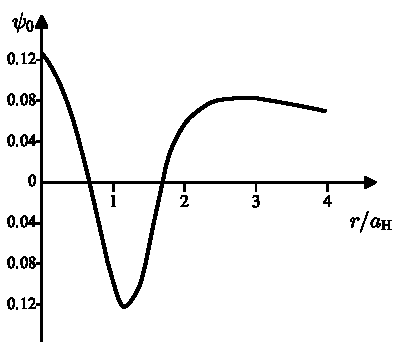
\includegraphics[width=6cm]{fig8-5.pdf}\\{\small 图 8.5\quad 金属Na导带底的维格纳-赛茨波函数}
\end{minipage}
\end{center}

金属的结合能由两部分组成：(i)自由原子的基态能 $E_{\mathrm{a}}$ 与导带底能量 $E_{0}$ 之差，(ii)导带中的电子平均动能等于 $\frac{3}{5}(\hbar^{2}k_{\mathrm{F}}^{2}/2m^{*})$，$m^{*}$ 为有效质量.金属Na的原子基态能 $E_{\mathrm{a}}$（即3s的电子能量）的实验测量值为 $-5.16$ eV，导带电子的平均动能
\begin{equation}
  \langle E_{\mathrm{F}}\rangle=\frac{3}{5}\frac{\hbar^{2}k_{\mathrm{F}}^{2}}{2m^{*}}
  =\frac{1.10}{r_{\mathrm{s}}^{2}}\frac{e^{2}}{a_{\mathrm{H}}}\Bigl(\frac{m}{m^{*}}\Bigr)
\end{equation}
若取 $m^{*}=m$，可算出 $\langle E_{\mathrm{F}}\rangle$ 约为 2.0 eV.由此求得的结合能为 $-1.1$ eV，与实验值 $-1.13$ eV 符合良好.

$E_{\mathrm{a}}$ 与 $E_{0}$ 的差别来源于边界条件的不同.对自由原子中电子边界条件应换为 $\left[\partial\psi_{0}(\boldsymbol{r})/\partial r\right]_{r=\infty}=0$，仍满足方程(8.5.12)，$V(r)$ 也取钠的离子实势.图8.6是Na的3s电子在自由原子状态（实线）和金属态（虚线）时波函数的示意图.显然，在固体中3s电子的分布更靠近离子实，因此有更低的势能，故 $|E_{0}|>|E_{\mathrm{a}}|$.

\begin{center}
\begin{minipage}{6cm}
\centering
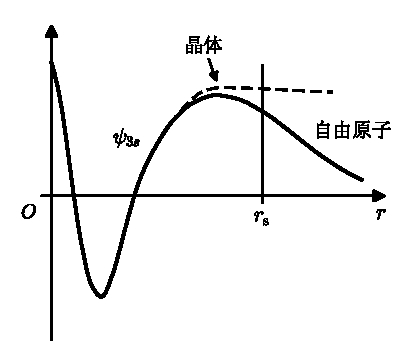
\includegraphics[width=6cm]{fig8-6.pdf}\\{\small 图 8.6\quad 维格纳-赛茨波函数和自由原子的3s波函数}
\end{minipage}
\end{center}
\subsection*{2. $\boldsymbol{k}=0$ 点附近有效质量的计算\textsuperscript{[11]}}

设价电子能带的底部在 $\boldsymbol{k}=0$ 处.为求得小 $k$ 状态的电子波函数和有效质量 $m^{*}$，应当从布洛赫函数
\begin{equation*}
  \psi_{\boldsymbol{k}}(\boldsymbol{r})=u_{\boldsymbol{k}}(\boldsymbol{r})\mathrm{e}^{\mathrm{i}\boldsymbol{k}\cdot\boldsymbol{r}}
\end{equation*}
出发，利用式(8.5.1)先写出 $u_{\boldsymbol{k}}(\boldsymbol{r})$ 所满足的方程
\begin{equation}
\begin{aligned}
  &-\frac{\hbar^{2}}{2m}(\nabla^{2}+2\mathrm{i}\boldsymbol{k}\cdot\nabla)u_{\boldsymbol{k}}(\boldsymbol{r})
  +V(\boldsymbol{r})u_{\boldsymbol{k}}(\boldsymbol{r})\\
  &\qquad=\Bigl(E-\frac{\hbar^{2}k^{2}}{2m}\Bigr)u_{\boldsymbol{k}}(\boldsymbol{r})
\end{aligned}
\end{equation}
其中 $u_{\boldsymbol{k}}(\boldsymbol{r})$ 是正点阵的周期函数.在W-S元胞内，$V(r)$ 为球形对称的离子实势.方程(8.5.14)与 $\psi_{0}(\boldsymbol{r})=u_{0}(r)$ 所满足的方程不同，其主要差别是出现了 $-\bigl(\mathrm{i}\hbar^{2}/m\bigr)\boldsymbol{k}\cdot\nabla u_{\boldsymbol{k}}$ 项，对于小 $k$ 值它可以当作微扰项处理.在讨论过程中仍可利用元胞法的球近似在 $0\leqslant r\leqslant r_{\mathrm{s}}$ 范围内作计算，并要求 $\psi_{0}$ 满足边界条件式(8.5.11).

将 $u_{\boldsymbol{k}}(\boldsymbol{r})$ 展开为 $k$ 的幂级数
\begin{equation}
\begin{aligned}
  u_{\boldsymbol{k}}(\boldsymbol{r})&=\sum_{n=0}^{\infty}u_{n}(\boldsymbol{r})k^{n}\\
  &=u_{0}(\boldsymbol{r})+u_{1}(\boldsymbol{r})k+\cdots\\
  &=\psi_{0}(\boldsymbol{r})+u_{1}(\boldsymbol{r})k+\cdots
\end{aligned}
\end{equation}
相似的，对于 $E_{k}$ 作展开，考虑到一级微扰能量正比于
\begin{equation}
  \int_{\Omega}\psi_{0}\boldsymbol{k}\cdot\nabla\psi_{0}\,\mathrm{d}\tau
  =\int_{\Omega}\psi_{0}\frac{\partial\psi_{0}}{\partial r}(\boldsymbol{k}\cdot\boldsymbol{r})\frac{1}{r}\,\mathrm{d}\tau=0
\end{equation}
是奇函数，故能量的一级修正等于零.准至 $k^{2}$ 项的 $E_{k}$ 展开式在球形近似下设为
\begin{equation}
  E_{k}=E_{0}+\alpha\,\frac{\hbar^{2}k^{2}}{2m}
\end{equation}
其中 $E_{0}$ 代表 $\boldsymbol{k}=0$ 的能量，$\alpha\equiv m/m^{*}$.将式(8.5.15)和(8.5.17)代入式(8.5.14)，求得 $\psi_{0}$ 与 $u_{1}$ 所满足的方程：
\begin{equation}
  \Bigl[-\nabla^{2}+\frac{2m}{\hbar^{2}}(V-E_{0})\Bigr]\psi_{0}=0
\end{equation}
\begin{equation}
  \Bigl[-\nabla^{2}+\frac{2m}{\hbar^{2}}(V-E_{0})\Bigr]u_{1}=2\mathrm{i}\,\boldsymbol{k}_{1}\cdot\nabla\psi_{0}
\end{equation}
其中 $\boldsymbol{k}_{1}$ 代表 $\boldsymbol{k}$ 方向单位矢
\begin{equation}
  \boldsymbol{k}_{1}\equiv\frac{\boldsymbol{k}}{k}
\end{equation}
设方程(8.5.18)的解 $\psi_{0}$ 和 $E_{0}$ 已经求得，现在主要任务是解方程(8.5.19).显然，$u_{1}(\boldsymbol{r})$ 是奇函数，又由于 $u_{1}(\boldsymbol{r})$ 应为正点阵的周期函数，因此经过W-S元胞多面体界面时，$u_{1}$ 将变号，这说明在边界面上 $u_{1}$ 必须等于零.若采用球近似可将 $u_{1}$ 的边界条件写为
\begin{equation}
  u_{1}(r)\Big|_{r=r_{\mathrm{s}}}=0
\end{equation}
式(8.5.19)的特解为
\begin{equation}
  -\mathrm{i}\,\boldsymbol{k}_{1}\cdot\boldsymbol{r}\,\psi_{0}(r)
\end{equation}
可直接代入方程(8.5.19)验证.为了满足边界条件式(8.5.21)，还必须加入式(8.5.19)的齐次方程解，可设其为
\begin{equation}
  \mathrm{i}(\boldsymbol{k}_{1}\cdot\boldsymbol{r}_{1})f_{\mathrm{p}}(r)\qquad
  \Bigl(\boldsymbol{r}_{1}\equiv\frac{\boldsymbol{r}}{r}\Bigr)
\end{equation}
将上式代入(8.5.19)，立刻得径向函数 $f_{\mathrm{p}}(r)$ 满足
\begin{equation}
  \frac{1}{r^{2}}\frac{\mathrm{d}}{\mathrm{d}r}\Bigl(r^{2}\frac{\mathrm{d}f_{\mathrm{p}}}{\mathrm{d}r}\Bigr)
  +\Bigl[\frac{2m}{\hbar^{2}}(E_{0}-V)-\frac{2}{r^{2}}\Bigr]f_{\mathrm{p}}=0
\end{equation}
与式(8.5.6)相比较可知，$f_{\mathrm{p}}$ 满足p波（$l=1$）的径向方程，式(8.5.23)也是反演操作的奇函数.因此，方程(8.5.19)的解为
\begin{equation}
  u_{1}(\boldsymbol{r})=\mathrm{i}(\boldsymbol{k}_{1}\cdot\boldsymbol{r})
  \Bigl[\frac{f_{\mathrm{p}}(r)}{r}-\psi_{0}(r)\Bigr]
\end{equation}
要求 $u_{1}(\boldsymbol{r})$ 满足边界条件式(8.5.21)，求得关系式
\begin{equation}
  f_{\mathrm{p}}(r_{\mathrm{s}})=r_{\mathrm{s}}\psi_{0}(r_{\mathrm{s}})
\end{equation}
利用求出的波函数代入式(8.5.15)，得
\begin{equation}
  \psi_{\boldsymbol{k}}(\boldsymbol{r})\approx\psi_{0}(\boldsymbol{r})+ku_{1}(\boldsymbol{r})
  =\psi_{0}+\mathrm{i}\,\boldsymbol{k}\cdot\boldsymbol{r}\,v(\boldsymbol{r})
\end{equation}
其中
\begin{equation}
  v(\boldsymbol{r})\equiv\frac{f_{\mathrm{p}}(r)}{r}-\psi_{0}(r)
\end{equation}
并设 $\psi_{\boldsymbol{k}}$ 满足归一条件
\begin{equation}
  \int_{\Omega}\psi_{\boldsymbol{k}}^{*}\psi_{\boldsymbol{k}}\,\mathrm{d}\tau=1
\end{equation}
则能带为
\begin{equation}
  E_{k}=\int_{\Omega}\psi_{\boldsymbol{k}}^{*}\Bigl[-\frac{\hbar^{2}}{2m}\nabla^{2}+V(\boldsymbol{r})\Bigr]\psi_{\boldsymbol{k}}\,\mathrm{d}\tau
\end{equation}
计算准至 $k^{2}$ 项的本征能量，可求得式(8.5.17)中的 $\alpha$ 为
\begin{equation}
  \alpha=1+\frac{2}{k^{2}}\int_{\Omega}\psi_{0}\Bigl[k^{2}v
  +\frac{1}{r}(\boldsymbol{k}\cdot\boldsymbol{r})^{2}\frac{\mathrm{d}v}{\mathrm{d}r}\Bigr]\mathrm{d}\tau
\end{equation}
这里 $\Omega$ 是W-S元胞，计算时近似取半径为 $r_{\mathrm{s}}$ 的球体.上式对角度积分后
\begin{equation}
  \alpha=1+8\pi\int_{0}^{r_{\mathrm{s}}}\psi_{0}(r)\Bigl[v(r)+\frac{r}{3}\Bigl(\frac{\mathrm{d}v}{\mathrm{d}r}\Bigr)\Bigr]r^{2}\,\mathrm{d}r
\end{equation}
再作部分积分，消去积分中第一项，得到
\begin{equation}
  \alpha=1-\frac{8\pi}{3}\int_{0}^{r_{\mathrm{s}}}v(r)\Bigl(\frac{\mathrm{d}\psi_{0}}{\mathrm{d}r}\Bigr)r^{3}\,\mathrm{d}r
\end{equation}
上式再经简化，可用 $r=r_{\mathrm{s}}$ 处的 $\psi_{0}$ 和 $v$ 表示 $\alpha$.为此，令
\begin{equation}
  \left.
  \begin{aligned}
    f_{\mathrm{p}}(r)&=\frac{P(r)}{r}\\
    \psi_{0}(r)&=\frac{R(r)}{r}
  \end{aligned}\right\}
\end{equation}
则
\begin{equation}
\begin{aligned}
  v(r)&=\frac{f_{\mathrm{p}}(r)}{r}-\psi_{0}(r)\\
  &=\frac{P(r)}{r^{2}}-\frac{R(r)}{r}
\end{aligned}
\end{equation}
相应的，将 $f_{\mathrm{p}}$ 与 $\psi_{0}$ 的方程(8.5.24)和(8.5.12)改写成
\begin{equation}
  \frac{\mathrm{d}^{2}R}{\mathrm{d}r^{2}}+\frac{2m}{\hbar^{2}}(E_{0}-V)R=0
\end{equation}
\begin{equation}
  \frac{\mathrm{d}^{2}P}{\mathrm{d}r^{2}}-\frac{2}{r^{2}}P+\frac{2m}{\hbar^{2}}(E_{0}-V)P=0
\end{equation}
用 $P(r)$ 和 $R(r)$ 表示的 $\alpha$ 为
\begin{equation}
  \alpha=1-\frac{8\pi}{3}\int_{0}^{r_{\mathrm{s}}}(P-rR)\Bigl(\frac{\mathrm{d}R}{\mathrm{d}r}-\frac{R}{r}\Bigr)\mathrm{d}r
\end{equation}
再利用下列关系式：

(i)由式(8.5.36)与(8.5.37)得
\begin{equation}
  R\Bigl(\frac{\mathrm{d}^{2}P}{\mathrm{d}r^{2}}\Bigr)-P\Bigl(\frac{\mathrm{d}^{2}R}{\mathrm{d}r^{2}}\Bigr)=\frac{2PR}{r^{2}}
\end{equation}

(ii)考虑 $\psi_{0}(\boldsymbol{r})=\dfrac{R(r)}{r}$ 在 $r_{\mathrm{s}}$ 球内近似归一
\begin{equation}
  \int_{\Omega}\psi_{0}^{2}\,\mathrm{d}\tau=\int_{0}^{r_{\mathrm{s}}}4\pi R^{2}(r)\,\mathrm{d}r\approx 1
\end{equation}
作分部积分可证明
\begin{equation}
  \frac{8\pi}{3}\int_{0}^{r_{\mathrm{s}}}rR\Bigl(\frac{\mathrm{d}R}{\mathrm{d}r}\Bigr)\mathrm{d}r
  =\frac{4\pi}{3}r_{\mathrm{s}}^{3}[\psi_{0}(r_{\mathrm{s}})]^{2}-\frac{1}{3}
\end{equation}

(iii)在 $r=r_{\mathrm{s}}$ 处 $\psi_{0}$ 满足 $\Bigl(\dfrac{\mathrm{d}\psi_{0}}{\mathrm{d}r}\Bigr)_{r_{\mathrm{s}}}=0$，$P(r_{\mathrm{s}})$ 的边界条件由式(8.5.26)和式(8.5.34)给出
\begin{equation}
  P(r_{\mathrm{s}})=r_{\mathrm{s}}R(r_{\mathrm{s}})
\end{equation}
可以证明
\begin{equation}
  \alpha=\gamma\Bigl[\Bigl(\frac{r}{P}\Bigr)\Bigl(\frac{\mathrm{d}P}{\mathrm{d}r}\Bigr)-1\Bigr]_{r=r_{\mathrm{s}}}
\end{equation}
其中
\begin{equation}
  \gamma\equiv\frac{4\pi}{3}r_{\mathrm{s}}^{3}[\psi_{0}(r_{\mathrm{s}})]^{2}
  =\frac{4\pi}{3}r_{\mathrm{s}}R^{2}(r_{\mathrm{s}})
\end{equation}
当 $\psi_{0}$ 已知时，只要从式(8.5.37)数值解出 $P(r)$，就能求得能带底部的有效质量 $m^{*}=m/\alpha$，从而得到 $\boldsymbol{k}=0$ 附近的电子能量.实际运算时，式(8.5.43)比式(8.5.33)更为方便.

元胞法的球近似尽管计算简单，但是所求得的结果仅与原子体积（或 $r_{\mathrm{s}}$）有关，它完全忽略了实际晶体结构的影响，假如计及晶体结构的影响，则必须使球函数的展开式在复杂的W-S元胞多面体界面上满足边界条件，对于BZ中的一般点，其数值计算工作量是相当大的，此外，从物理上看，在整个W-S元胞内都采用球对称的离子实势，也存在问题，因为W-S近似的势场在元胞边界处有导数的不连续性，如图8.7中实线所示.但是，实际上在这些地方势能的变化十分平滑，近似为常数势，如图8.7中虚线所示.鉴于以上困难，近年来元胞法已很少被采用，而代之以克服了上述缺点的新方法，例如格林函数方法和缀加平面波法.

\begin{center}
\begin{minipage}{6cm}
\centering
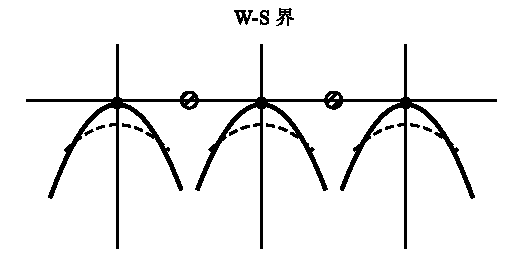
\includegraphics[width=6cm]{fig8-7.pdf}\\{\small 图 8.7\quad 元胞法势}
\end{minipage}
\end{center}
\section{缀加平面波法}

为了克服元胞法在W-S多面体上满足边界条件的困难，斯莱特（Slater）\textsuperscript{[12]}建议用丸盒势（muffin-tin potential）模型处理问题.所谓丸盒势即假定W-S元胞中球对称势仅限于离子实周围半径 $r_{\mathrm{i}}$ 的球体内，这些球彼此不相交如图8.8所示，称为M-T球.在M-T球外的元胞势场，则假定为常数势.适当选择能量的零点，可将W-S元胞内的丸盒势简单写成

\begin{center}
\begin{minipage}{5.5cm}
\centering
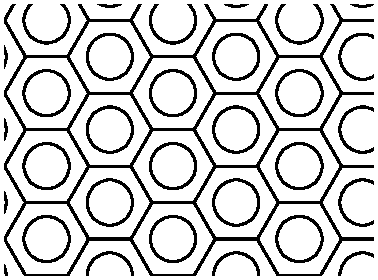
\includegraphics[width=5.5cm]{fig8-8.pdf}\\{\small 图 8.8\quad M-T球}
\end{minipage}
\end{center}

\begin{equation}
  V_{\mathrm{M\text{-}T}}(r)=\begin{cases}
    V(r) & (r<r_{\mathrm{i}})\\[0.2em]
    0 & (r\geqslant r_{\mathrm{i}})
  \end{cases}
\end{equation}
其中 $V(r)$ 是球对称的离子实势场，图8.9绘出了沿某离子线的丸盒势图.丸盒势模型将M-T球外的势场取为常数，显然更逼近实际情况，因为在这些地方薛定谔方程的解是平面波，而平面波在W-S多面体上能自动满足边界条件式(8.5.2)和(8.5.3).因此，丸盒势模型克服了元胞法满足边界条件的困难.在每个M-T球内，由于是球对称的势场，薛定谔方程的严格解可用径向波函数与球谐函数的乘积来展开表示

\begin{center}
\begin{minipage}{6cm}
\centering
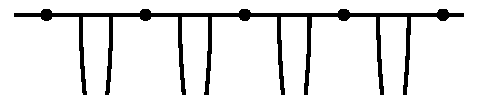
\includegraphics[width=6cm]{fig8-9.pdf}\\{\small 图 8.9\quad M-T势 $V_{\mathrm{M\text{-}T}}$}
\end{minipage}
\end{center}

\begin{equation}
  \phi_{\boldsymbol{k}}(\boldsymbol{r})=\begin{cases}
    \displaystyle\sum_{l,\,m}\mathrm{i}^{l}a_{lm}(\boldsymbol{k})\mathrm{Y}_{lm}(\theta,\phi)R_{l}(E_{k},r)
    & (r\leqslant r_{\mathrm{i}})\\[1.2em]
    \exp(\mathrm{i}\,\boldsymbol{k}\cdot\boldsymbol{r}) & (r>r_{\mathrm{i}})
  \end{cases}
\end{equation}
其中 $R_{l}(E_{k},r)$ 满足径向薛定谔方程
\begin{equation}
  \frac{1}{r^{2}}\frac{\mathrm{d}}{\mathrm{d}r}\Bigl(r^{2}\frac{\mathrm{d}R_{l}}{\mathrm{d}r}\Bigr)
  +\Bigl[\frac{2m}{\hbar^{2}}\bigl(E-V(r)\bigr)-\frac{l(l+1)}{r^{2}}\Bigr]R_{l}=0
\end{equation}
剩下的问题是如何使式(8.6.2)中的平面波与M-T球内球函数展开式相衔接.斯莱特要求 $\phi_{\boldsymbol{k}}(\boldsymbol{r})$ 在 $r=r_{\mathrm{i}}$ 处连续，从而决定系数 $a_{lm}$.将平面波用球谐函数展开：
\begin{equation}
  \mathrm{e}^{\mathrm{i}\boldsymbol{k}\cdot\boldsymbol{r}}=4\pi\sum_{l,\,m}\mathrm{i}^{l}\mathrm{j}_{l}(kr)\mathrm{Y}_{lm}(\theta,\phi)\mathrm{Y}_{lm}^{*}(\theta_{k},\phi_{k})
\end{equation}
其中 $(\theta,\phi)$ 是矢量 $\boldsymbol{r}$ 的方位角，$(\theta_{k},\phi_{k})$ 是 $\boldsymbol{k}$ 的方位角，$\mathrm{j}_{l}$ 为球贝塞尔函数，利用式(8.6.2)和 $r=r_{\mathrm{i}}$ 处 $\phi_{\boldsymbol{k}}$ 连续的条件，求得
\begin{equation}
  a_{lm}(\boldsymbol{k})=4\pi\mathrm{i}^{l}\bigl[\mathrm{j}_{l}(kr_{\mathrm{i}})/R_{l}(E_{k},r_{\mathrm{i}})\bigr]\mathrm{Y}_{lm}^{*}(\theta_{k},\phi_{k})
\end{equation}
将式(8.6.5)代入式(8.6.2)，所组成的 $\phi_{\boldsymbol{k}}(\boldsymbol{r})$ 称为缀加平面波（简称APW）.应当注意，APW与OPW不同之处在于平面波与球函数只在 $r=r_{\mathrm{i}}$ 处相接，而无重叠区.

晶体中单电子的布洛赫函数可由APW作基函数展开表示：
\begin{equation}
  \psi_{\boldsymbol{k}}(\boldsymbol{r})=\sum_{\boldsymbol{K}}\alpha(\boldsymbol{k}+\boldsymbol{K})\phi_{\boldsymbol{k}+\boldsymbol{K}}(\boldsymbol{r})
\end{equation}

\begin{center}
\begin{minipage}{6cm}
\centering
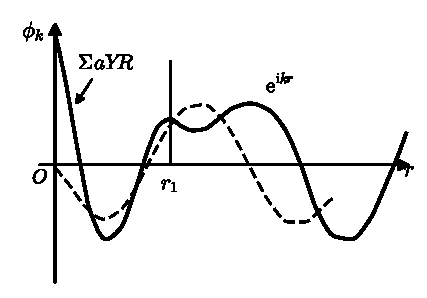
\includegraphics[width=6cm]{fig8-10.pdf}\\{\small 图 8.10\quad APW示意图}
\end{minipage}
\end{center}

其中 $\alpha(\boldsymbol{k}+\boldsymbol{K})$ 为待定系数，$\boldsymbol{K}$ 为倒格矢，而APW可根据式(8.6.2)与(8.6.5)写成
\begin{equation}
\begin{aligned}
  \phi_{\boldsymbol{k}+\boldsymbol{K}}(\boldsymbol{r})
  &=\mathrm{e}^{\mathrm{i}(\boldsymbol{k}+\boldsymbol{K})\cdot\boldsymbol{r}}\eta(\boldsymbol{r}-\boldsymbol{r}_{\mathrm{i}})
  +\eta(\boldsymbol{r}_{\mathrm{i}}-\boldsymbol{r})\sum_{l,\,m}4\pi\mathrm{i}^{l}\mathrm{j}_{l}(|\boldsymbol{k}+\boldsymbol{K}|\,r_{\mathrm{i}})\cdot\\
  &\qquad\Bigl[\frac{R_{l}(E_{k},\boldsymbol{r})}{R_{l}(E_{k},r_{\mathrm{i}})}\Bigr]\mathrm{Y}_{lm}(\theta,\phi)\mathrm{Y}_{lm}^{*}(\theta_{k},\phi_{k})
\end{aligned}
\end{equation}
这里 $\eta(x)$ 是阶跃函数：
\begin{equation}
  \eta(x)=\begin{cases}
    1 & (x>0)\\
    0 & (x<0)
  \end{cases}
\end{equation}
由于 $\phi_{\boldsymbol{k}+\boldsymbol{K}}(\boldsymbol{r})$ 在 $r=r_{\mathrm{i}}$ 处具有导数不连续性，应当利用附录G中的变分原理来确定 $E_{k}$ 和系数 $\alpha(\boldsymbol{k}+\boldsymbol{K})$.具体做法如下：

（i）以 $\psi_{\boldsymbol{k}}=\sum_{\boldsymbol{K}}\alpha(\boldsymbol{k}+\boldsymbol{K})\phi_{\boldsymbol{k}+\boldsymbol{K}}$ 作为试探变分函数，代入能量泛函公式［见式(G.3)］
\begin{equation}
  \int_{\Omega}\Bigl\{\frac{\hbar^{2}}{2m}|\nabla\psi_{\boldsymbol{k}}|^{2}+V|\psi_{\boldsymbol{k}}|^{2}\Bigr\}\mathrm{d}\tau
  -E[\psi_{\boldsymbol{k}}]\int_{\Omega}\psi_{\boldsymbol{k}}^{*}\psi_{\boldsymbol{k}}\,\mathrm{d}\tau=0
\end{equation}

（ii）作变分时应要求泛函 $E[\psi_{\boldsymbol{k}}]$ 对于 $\psi_{\boldsymbol{k}}$ 是稳定的，这时 $E$ 才是晶体中单电子薛定谔方程的能带解.当 $\alpha^{*}$ 变化时，这一要求简单表示为
\begin{equation}
  \frac{\partial E[\psi_{\boldsymbol{k}}]}{\partial\alpha^{*}}=0
\end{equation}

（iii）式(8.6.9)对 $\alpha^{*}$ 变分，并利用式(8.6.10)，可求得 $\alpha(\boldsymbol{k}+\boldsymbol{K})$ 的线性齐次方程组
\begin{equation}
  \sum_{\boldsymbol{K}'}\langle\boldsymbol{k}+\boldsymbol{K}|M|\boldsymbol{k}+\boldsymbol{K}'\rangle_{\mathrm{APW}}\alpha(\boldsymbol{k}+\boldsymbol{K}')=0
\end{equation}
其中
\begin{equation}
\begin{aligned}
  &\langle\boldsymbol{k}+\boldsymbol{K}|M|\boldsymbol{k}+\boldsymbol{K}'\rangle_{\mathrm{APW}}\\
  &\quad=\int_{\Omega}\mathrm{d}\tau\Bigl\{\frac{\hbar^{2}}{2m}\nabla\phi_{\boldsymbol{k}+\boldsymbol{K}}^{*}\cdot\nabla\phi_{\boldsymbol{k}+\boldsymbol{K}'}
  +(V-E)\phi_{\boldsymbol{k}+\boldsymbol{K}}^{*}\phi_{\boldsymbol{k}+\boldsymbol{K}'}\Bigr\}
\end{aligned}
\end{equation}
这里 $\boldsymbol{K}$、$\boldsymbol{K}'$ 均为倒格矢.

（iv）能量本征值 $E_{k}$ 由式(8.6.11)的系数行列式等于零决定：
\begin{equation}
  \mathrm{det}\,\|\langle\boldsymbol{k}+\boldsymbol{K}|M|\boldsymbol{k}+\boldsymbol{K}'\rangle_{\mathrm{APW}}\|=0
\end{equation}
具体计算 $M$ 的APW矩阵元时，应将元胞 $\Omega$ 分为M-T球内部分 $\Omega_{\mathrm{I}}=\dfrac{4\pi}{3}r_{\mathrm{i}}^{3}$ 和球外部分 $\Omega_{\mathrm{II}}$：
\begin{equation}
  \Omega=\Omega_{\mathrm{I}}+\Omega_{\mathrm{II}}
\end{equation}
由于 $r_{\mathrm{i}}$ 球外部分 $V(\boldsymbol{r})=0$，$\phi_{\boldsymbol{k}+\boldsymbol{K}}$ 为平面波 $\mathrm{e}^{\mathrm{i}(\boldsymbol{k}+\boldsymbol{K})\cdot\boldsymbol{r}}$，其计算十分方便.将式(8.6.1)和(8.6.2)代入式(8.6.12)，可将球外APW对 $M$ 矩阵元的贡献写成
\begin{equation}
\begin{aligned}
  &\Bigl(\int_{\Omega}-\int_{\Omega_{\mathrm{I}}}\Bigr)\mathrm{d}\tau
  \Bigl\{\frac{\hbar^{2}}{2m}\nabla\mathrm{e}^{-\mathrm{i}(\boldsymbol{k}+\boldsymbol{K})\cdot\boldsymbol{r}}\cdot\nabla\mathrm{e}^{\mathrm{i}(\boldsymbol{k}+\boldsymbol{K}')\cdot\boldsymbol{r}}
  -E\,\mathrm{e}^{\mathrm{i}(\boldsymbol{K}'-\boldsymbol{K})\cdot\boldsymbol{r}}\Bigr\}\\
  &\quad=\Bigl[\frac{\hbar^{2}}{2m}(\boldsymbol{k}+\boldsymbol{K})\cdot(\boldsymbol{k}+\boldsymbol{K}')-E\Bigr]
  \Bigl\{\int_{\Omega}\mathrm{e}^{\mathrm{i}(\boldsymbol{K}'-\boldsymbol{K})\cdot\boldsymbol{r}}\mathrm{d}\tau\\
  &\qquad-\int_{\Omega_{\mathrm{I}}}\mathrm{e}^{\mathrm{i}(\boldsymbol{K}'-\boldsymbol{K})\cdot\boldsymbol{r}}\mathrm{d}\tau\Bigr\}
\end{aligned}
\end{equation}
利用关系式
\begin{equation}
  \int_{\Omega}\mathrm{e}^{\mathrm{i}(\boldsymbol{K}'-\boldsymbol{K})\cdot\boldsymbol{r}}\mathrm{d}\tau=\Omega\,\delta_{\boldsymbol{K}\boldsymbol{K}'}
\end{equation}
和
\begin{equation}
  \int_{\Omega_{\mathrm{I}}}\mathrm{e}^{\mathrm{i}\boldsymbol{p}\cdot\boldsymbol{r}}\mathrm{d}\tau
  =4\pi\int_{0}^{r_{\mathrm{i}}}\Bigl(\frac{\sin pr}{pr}\Bigr)r^{2}\,\mathrm{d}r
  =4\pi r_{\mathrm{i}}^{2}\frac{\mathrm{j}_{1}(pr_{\mathrm{i}})}{p}
\end{equation}
最后求得平面波部分对 $M$ 的贡献为
\begin{equation}
  \Bigl\{\frac{\hbar^{2}}{2m}(\boldsymbol{k}+\boldsymbol{K})\cdot(\boldsymbol{k}+\boldsymbol{K}')-E\Bigr\}
  \Bigl\{\Omega\delta_{\boldsymbol{K}\boldsymbol{K}'}
  -4\pi r_{\mathrm{i}}^{2}\frac{\mathrm{j}_{1}(|\boldsymbol{K}'-\boldsymbol{K}|\,r_{\mathrm{i}})}{|\boldsymbol{K}'-\boldsymbol{K}|}\Bigr\}
\end{equation}
球内部分 $M$ 矩阵元的计算比较复杂，这里只说明步骤.对式(8.6.12)右边第一项作部分积分，并利用格林定理，得到关系式
\begin{equation}
\begin{aligned}
  \int_{\Omega_{\mathrm{I}}}\nabla\phi_{\boldsymbol{k}+\boldsymbol{K}}^{*}\cdot\nabla\phi_{\boldsymbol{k}+\boldsymbol{K}'}\,\mathrm{d}\tau&\\
  =\int_{\Omega_{\mathrm{I}}}\phi_{\boldsymbol{k}+\boldsymbol{K}}^{*}(-\nabla^{2})\phi_{\boldsymbol{k}+\boldsymbol{K}'}\,\mathrm{d}\tau
  +\int_{S}\phi_{\boldsymbol{k}+\boldsymbol{K}}^{*}\nabla\phi_{\boldsymbol{k}+\boldsymbol{K}'}\cdot\mathrm{d}\boldsymbol{S}&
\end{aligned}
\end{equation}
其中 $S$ 代表 $r_{\mathrm{i}}$ 球面，则 $\langle\boldsymbol{k}+\boldsymbol{K}|M|\boldsymbol{k}+\boldsymbol{K}'\rangle_{\mathrm{APW}}$ 的球内部分贡献可表示为
\begin{equation}
  \int_{\Omega_{\mathrm{I}}}\nabla\phi_{\boldsymbol{k}+\boldsymbol{K}}^{*}\Bigl[-\frac{\hbar^{2}}{2m}\nabla^{2}+V(r)-E\Bigr]\phi_{\boldsymbol{k}+\boldsymbol{K}'}\,\mathrm{d}\tau
  +\int_{S}\phi_{\boldsymbol{k}+\boldsymbol{K}}^{*}\frac{\partial}{\partial\eta}\phi_{\boldsymbol{k}+\boldsymbol{K}'}\,\mathrm{d}S
\end{equation}
面积分中的 $\eta$ 是M-T球面的外法线.式(8.6.20)中的体积分等于零.因为在 $r<r_{\mathrm{i}}$ 时 $(H-E)\phi_{\boldsymbol{k}+\boldsymbol{K}'}=0$ 与径向方程(8.6.3)一致，这说明APW在M-T球内满足薛定谔方程.面积分部分要利用球函数的正交条件及其辅助定理，斯莱特计算的最后结果为
\begin{equation}
\begin{aligned}
  4\pi r_{\mathrm{i}}^{2}\sum_{l=0}^{\infty}(2l+1)\mathrm{P}_{l}(\cos\theta_{\boldsymbol{K}\boldsymbol{K}'})\mathrm{j}_{l}(|\boldsymbol{k}+\boldsymbol{K}|\,r_{\mathrm{i}})\times\\
  \mathrm{j}_{l}(|\boldsymbol{k}+\boldsymbol{K}'|\,r_{\mathrm{i}})\frac{R_{l}'(E,r_{\mathrm{i}})}{R_{l}(E,r_{\mathrm{i}})}
\end{aligned}
\end{equation}
其中 $R_{l}'\equiv\dfrac{\mathrm{d}R_{l}}{\mathrm{d}r}$，$\theta_{\boldsymbol{K}\boldsymbol{K}'}$ 为 $\boldsymbol{K}$ 与 $\boldsymbol{K}'$ 间夹角，具体推导可参考原文\textsuperscript{[19]}.式(8.6.21)与式(8.6.18)之和即是 $\langle\boldsymbol{k}+\boldsymbol{K}|M|\boldsymbol{k}+\boldsymbol{K}'\rangle_{\mathrm{APW}}$，可整理成对角及非对角部分之和
\begin{equation}
  \frac{1}{\Omega}\langle\boldsymbol{k}+\boldsymbol{K}|M|\boldsymbol{k}+\boldsymbol{K}'\rangle_{\mathrm{APW}}
  =\Bigl[\frac{\hbar^{2}}{2m}(\boldsymbol{k}+\boldsymbol{K})^{2}-E\Bigr]\delta_{\boldsymbol{K}\boldsymbol{K}'}
  +\Gamma_{\boldsymbol{K}\boldsymbol{K}'}
\end{equation}
这里非对角矩阵元 $\Gamma_{\boldsymbol{K}\boldsymbol{K}'}$ 定义为
\begin{equation}
\begin{aligned}
  \Gamma_{\boldsymbol{K}\boldsymbol{K}'}&\equiv\frac{4\pi r_{\mathrm{i}}^{2}}{\Omega}\biggl\{
  -\Bigl[\frac{\hbar^{2}}{2m}(\boldsymbol{k}+\boldsymbol{K})\cdot(\boldsymbol{k}+\boldsymbol{K}')-E\Bigr]
  \frac{\mathrm{j}_{1}(|\boldsymbol{K}'-\boldsymbol{K}|\,r_{\mathrm{i}})}{|\boldsymbol{K}'-\boldsymbol{K}|}\\
  &\quad+\sum_{l=0}^{\infty}(2l+1)\mathrm{P}_{l}(\cos\theta_{\boldsymbol{K}\boldsymbol{K}'})\mathrm{j}_{l}(|\boldsymbol{k}+\boldsymbol{K}|\,r_{\mathrm{i}})\cdot\\
  &\qquad\mathrm{j}_{l}(|\boldsymbol{k}+\boldsymbol{K}'|\,r_{\mathrm{i}})\frac{R_{l}'(E,r_{\mathrm{i}})}{R_{l}(E,r_{\mathrm{i}})}\biggr\}
\end{aligned}
\end{equation}
根据式(8.6.22)的记号，可将方程(8.6.11)写成与平面波法中式(8.1.11)相似的形式
\begin{equation}
  \Bigl\{\frac{\hbar^{2}(\boldsymbol{k}+\boldsymbol{K})^{2}}{2m}-E\Bigr\}_{\boldsymbol{K}}\alpha(\boldsymbol{k}+\boldsymbol{K})
  +\sum_{\boldsymbol{K}'(\boldsymbol{K}'\neq\boldsymbol{K})}\Gamma_{\boldsymbol{K}\boldsymbol{K}'}\alpha(\boldsymbol{k}+\boldsymbol{K}')=0
\end{equation}
类似的，久期方程(8.6.13)变为与(8.1.13)相似的表示式
\begin{equation}
  \mathrm{det}\,\Bigl\|\Bigl[\frac{\hbar^{2}}{2m}(\boldsymbol{k}+\boldsymbol{K})^{2}-E\Bigr]\delta_{\boldsymbol{K}\boldsymbol{K}'}
  +\Gamma_{\boldsymbol{K}\boldsymbol{K}'}\Bigr\|=0
\end{equation}
显然，$\Gamma_{\boldsymbol{K}\boldsymbol{K}'}$ 相当于有效势的傅里叶分量，由于APW法将M-T球外的平面波与M-T球内的原子波函数在 $r=r_{\mathrm{i}}$ 处连续相接，同样也将在离子实区引进振荡，与OPW有相似之处.因此，式(8.6.23)中的 $\Gamma_{\boldsymbol{K}\boldsymbol{K}'}$ 与OPW法中的 $\langle\boldsymbol{k}+\boldsymbol{K}|U|\boldsymbol{k}+\boldsymbol{K}'\rangle$［见式(8.2.14)］应有相似的抵消特性，就是说用APW法展开来表示 $\psi_{\boldsymbol{k}}$ 也具有比平面波方法收敛更快的优点.

应当指出，由于APW波函数是彼此不正交的，久期行列式(8.6.25)中对角与非对角元都明显含 $E$，此外能量 $E$ 还在 $\Gamma_{\boldsymbol{K}\boldsymbol{K}'}$ 表示式的 $R_{l}'(E,r_{\mathrm{i}})/R_{l}(E,r_{\mathrm{i}})$ 函数中出现.因此，利用APW法作能带计算时，首先要在能量 $E$ 时解出径向薛定谔方程(8.6.3)，并算出M-T球面上 $R_{l}$ 的对数导数值
\begin{equation*}
  \frac{\mathrm{d}}{\mathrm{d}r}\bigl\{\ln R_{l}(E,r)\bigr\}_{r=r_{\mathrm{i}}}=R_{l}'(E,r_{\mathrm{i}})/R_{l}(E,r_{\mathrm{i}})
\end{equation*}
然后，对于给定的波矢 $\boldsymbol{k}$ 按式(8.6.23)计算不同倒格矢之间的矩阵元，调整 $E$，直到久期行列式等于零时，才能定出能带电子的能量本征值 $E_{k}$.显然，这一计算过程的工作量相当大.但是，在电子计算机高度发展的今日已非难事，特别是在式(8.6.23)中出现的都是一些标准函数，它们都有现成的子程序可利用.此外，还可以利用晶体对称性降低久期行列式的维数，使计算简化.APW法既具有元胞法便于利用对称性的优点，又克服了元胞法在W-S元胞面上满足边界条件的困难.实践证明，APW法用于金属能带的计算是相当成功的，所算出的能带结构和费密面与实验符合良好\textsuperscript{[14]}，包括含d带的贵金属（Cu、Ag、Au）和过渡金属，而对于这些金属OPW法却不能应用.

APW法不适用于共价键半导体，这是与丸盒势模型密切有关的.对于呈密排结构的单价金属，可以认为在离子周围势场是球对称的，而在离子之间势场变化缓慢，因此M-T势适用于这些金属.但是，对于共价键晶体，如Ge、Si等属于四面体键，其原子势场的方向性变化很大，原子周围的势场既不是球对称的，而且在原子之间势场也不是缓慢变化的，与丸盒势模型差异较大，因此，APW法不能应用.
\section{KKR方法}

这是柯林嘎（Korringa）\textsuperscript{[15]}、孔恩（Kohn）和罗斯托克尔（Rostoker）\textsuperscript{[16]}所提出的另一种计算能带的有效方法，通常称为格林函数方法，或简称KKR法.KKR法与前面所介绍的能带计算法不同，它不是根据物理情况选择展开基函数，而是先把单电子运动方程化为积分方程，再用散射方法求解能态.其主要内容如下：

为了求解能带电子的薛定谔方程
\begin{equation}
  \Bigl(\frac{\hbar^{2}}{2m}\nabla^{2}+E\Bigr)\psi_{\boldsymbol{k}}(\boldsymbol{r})=V(\boldsymbol{r})\psi_{\boldsymbol{k}}(\boldsymbol{r})
\end{equation}
引入下列点源势方程
\begin{equation}
  \Bigl(\frac{\hbar^{2}}{2m}\nabla^{2}+E\Bigr)G(\boldsymbol{r},\boldsymbol{r}')=\delta(\boldsymbol{r}-\boldsymbol{r}')
\end{equation}
其中 $G(\boldsymbol{r},\boldsymbol{r}')$ 是单电子薛定谔方程的格林函数，式(8.7.2)又称为格林函数方程.利用 $G(\boldsymbol{r},\boldsymbol{r}')$ 可将微分方程(8.7.1)改写为积分方程
\begin{equation}
  \psi_{\boldsymbol{k}}(\boldsymbol{r})=\int_{\Omega}G(\boldsymbol{r},\boldsymbol{r}')V(\boldsymbol{r}')\psi_{\boldsymbol{k}}(\boldsymbol{r}')\,\mathrm{d}^{3}r'
\end{equation}
若用算子 $\Bigl(\dfrac{\hbar^{2}}{2m}\nabla^{2}+E\Bigr)$ 作用于式(8.7.3)的两边，再利用 $G(\boldsymbol{r},\boldsymbol{r}')$ 的方程(8.7.2)，可以立刻导出式(8.7.1)：
\begin{equation*}
\begin{aligned}
  \Bigl(\frac{\hbar^{2}}{2m}\nabla^{2}+E\Bigr)\psi_{\boldsymbol{k}}(\boldsymbol{r})
  &=\int_{\Omega}\Bigl[\Bigl(\frac{\hbar^{2}}{2m}\nabla^{2}+E\Bigr)G(\boldsymbol{r},\boldsymbol{r}')\Bigr]V(\boldsymbol{r}')\psi_{\boldsymbol{k}}(\boldsymbol{r}')\,\mathrm{d}^{3}r'\\
  &=\int_{\Omega}\delta(\boldsymbol{r}-\boldsymbol{r}')V(\boldsymbol{r}')\psi_{\boldsymbol{k}}(\boldsymbol{r}')\,\mathrm{d}^{3}r'\\
  &=V(\boldsymbol{r})\psi_{\boldsymbol{k}}(\boldsymbol{r})
\end{aligned}
\end{equation*}
说明式(8.7.3)与式(8.7.1)是等效的表示式.KKR方法的特点是利用式(8.7.3)，由格林函数 $G(\boldsymbol{r},\boldsymbol{r}')$ 求 $\psi_{\boldsymbol{k}}(\boldsymbol{r})$ 和 $E_{n}(\boldsymbol{k})$.

为了使所求得 $\psi_{\boldsymbol{k}}(\boldsymbol{r})$ 满足布洛赫定理，KKR要求晶体的 $G(\boldsymbol{r},\boldsymbol{r}')$ 也满足布洛赫定理
\begin{equation}
  G(\boldsymbol{r}+\boldsymbol{l},\boldsymbol{r}')=\mathrm{e}^{\mathrm{i}\boldsymbol{k}\cdot\boldsymbol{l}}G(\boldsymbol{r},\boldsymbol{r}')
\end{equation}
这是格林函数所满足的边界条件.根据量子力学\textsuperscript{[17]}，$G(\boldsymbol{r},\boldsymbol{r}')$ 由公式
\begin{equation}
  G(\boldsymbol{r},\boldsymbol{r}')=\sum_{j}\phi_{j}^{*}(\boldsymbol{r}')(E-E_{j})^{-1}\phi_{j}(\boldsymbol{r})
\end{equation}
决定，其中 $\phi_{j}$ 与 $E_{j}$ 代表式(8.7.2)的齐次方程的本征函数和本征值，满足方程
\begin{equation}
  \Bigl(\frac{\hbar^{2}}{2m}\nabla^{2}+E_{j}\Bigr)\phi_{j}(\boldsymbol{r})=0
\end{equation}
和完备性条件
\begin{equation}
  \sum_{j}\phi_{j}^{*}(\boldsymbol{r}')\phi_{j}(\boldsymbol{r})=\delta(\boldsymbol{r}-\boldsymbol{r}')
\end{equation}
不难验证，$G(\boldsymbol{r},\boldsymbol{r}')$ 的解式(8.7.5)满足格林函数方程(8.7.2)，因为从式(8.7.5)出发，利用式(8.7.6)和式(8.7.7)，能立刻求出式(8.7.2)：
\begin{equation*}
  \Bigl(\frac{\hbar^{2}}{2m}\nabla^{2}+E\Bigr)G(\boldsymbol{r},\boldsymbol{r}')
  =\sum_{j}\frac{\phi_{j}^{*}(\boldsymbol{r}')\Bigl(\dfrac{\hbar^{2}}{2m}\nabla^{2}+E\Bigr)\phi_{j}(\boldsymbol{r})}{E-E_{j}}
  =\sum_{j}\phi_{j}^{*}(\boldsymbol{r}')\phi_{j}(\boldsymbol{r})=\delta(\boldsymbol{r}-\boldsymbol{r}')
\end{equation*}
应注意，式(8.7.6)实际上是自由电子的定态薛定谔方程，因此满足布洛赫定理的 $\phi_{j}(\boldsymbol{r})$ 应取为
\begin{equation}
  \phi_{j}(\boldsymbol{r})=\Omega^{-1/2}\exp\bigl[\mathrm{i}(\boldsymbol{k}+\boldsymbol{K})\cdot\boldsymbol{r}\bigr]
\end{equation}
代表在元胞 $\Omega$ 内归一的一平面波，$\boldsymbol{k}\in\mathrm{BZ}$，而 $\boldsymbol{K}$ 为倒格矢.将上式代入式(8.7.5)，求得满足式(8.7.4)的格林函数.
\begin{equation}
  G(\boldsymbol{r},\boldsymbol{r}')=\frac{1}{\Omega}\sum_{\boldsymbol{K}}
  \frac{\exp\bigl[\mathrm{i}(\boldsymbol{k}+\boldsymbol{K})\cdot(\boldsymbol{r}-\boldsymbol{r}')\bigr]}
  {E-\dfrac{\hbar^{2}}{2m}(\boldsymbol{k}+\boldsymbol{K})^{2}}
\end{equation}
应当看到，对于确定的 $E$ 和 $\boldsymbol{k}$，这个 $\boldsymbol{K}$ 的求和式只因晶体结构而异.因此，$G(\boldsymbol{r},\boldsymbol{r}')$ 又称为结构格林函数.KKR法的主要步骤为，首先严格计算结构格林函数的求和式(8.7.9)，再由 $G$ 近似定 $E_{n}(\boldsymbol{k})$ 和 $\psi_{\boldsymbol{k}}(\boldsymbol{r})$.

作具体计算时，与缀加平面波法相同，也采用M-T势作近似.这时，由于在M-T球外 $V(\boldsymbol{r})=0\ (r>r_{\mathrm{i}})$，因此确定 $\psi_{\boldsymbol{k}}(\boldsymbol{r})$ 的方程只需在M-T球内积分
\begin{equation}
  \psi_{\boldsymbol{k}}(\boldsymbol{r})=\int_{r'\leqslant r_{\mathrm{i}}-\varepsilon}
  G(\boldsymbol{r},\boldsymbol{r}')V(\boldsymbol{r}')\psi_{\boldsymbol{k}}(\boldsymbol{r}')\,\mathrm{d}^{3}r'
  \qquad(\varepsilon=0^{+})
\end{equation}
再考虑到 $r<r_{\mathrm{i}}$ 时，$V(r)=V(r)$，代表球对称的离子实势，我们可以假定M-T球内能带电子波函数由球谐函数展开表示
\begin{equation}
  \psi_{\boldsymbol{k}}(\boldsymbol{r})=\sum_{l,\,m}C_{lm}R_{l}(r)\mathrm{Y}_{lm}(\theta,\phi)
\end{equation}
其中系数 $C_{lm}$ 待定.为导出 $C_{lm}$ 的方程，相应的将M-T球内 $G(\boldsymbol{r},\boldsymbol{r}')$ 也用球谐函数表示\textsuperscript{[18]}
\begin{equation}
\begin{aligned}
  G(\boldsymbol{r},\boldsymbol{r}')
  =\sum_{lm}\sum_{l'm'}&\bigl\{\mathrm{i}^{l-l'}A_{lm,\,l'm'}\mathrm{j}_{l}(gr)\mathrm{j}_{l'}(gr')\\
  &+g\,\delta_{ll'}\delta_{mm'}\mathrm{j}_{l}(gr)\mathrm{n}_{l'}(gr')\bigr\}\times\\
  &\mathrm{Y}_{lm}(\theta,\phi)\mathrm{Y}_{l'm'}^{*}(\theta',\phi')\qquad(r<r'<r_{\mathrm{i}})
\end{aligned}
\end{equation}
其中 $\mathrm{n}_{l}$ 是 $l$ 阶诺伊曼（Neumann）函数，当取里德伯原子单位时\footnote{当取 $1\,[\mathrm{Ry}]=(\hbar^{2}/2ma_{\mathrm{H}}^{2})=(e^{2}/2a_{\mathrm{H}})$ 作为能量的单位时，相当于取 $\hbar=2m=1$，$e^{2}=2$ 和 $a_{\mathrm{H}}$ 为长度的单位.}，$g$ 代表能量因子
\begin{equation}
  g=\sqrt{E}\ \ (E>0);\qquad g=\mathrm{i}\sqrt{(-E)}\ \ (E<0)
\end{equation}
而常数 $A_{lm,\,l'm'}$ 可按标准方法计算\textsuperscript{[19]}，它们只与晶体结构有关，因此 $A_{lm,\,l'm'}$ 称为结构常数.属于同类型点阵的不同晶体，$A_{lm,\,l'm'}$ 的计算只需进行一次，这是KKR方法在计算上的优点之一.

利用式(8.7.1)和式(8.7.2)，消去式(8.7.10)中的M-T势，再由积分的格林定理容易求出下列面积分等式：
\begin{equation}
  \int_{r_{\mathrm{i}}-\varepsilon}\bigl\{G(\boldsymbol{r},\boldsymbol{r}')\nabla'\psi_{\boldsymbol{k}}(\boldsymbol{r}')
  -\psi_{\boldsymbol{k}}(\boldsymbol{r}')\nabla'G(\boldsymbol{r},\boldsymbol{r}')\bigr\}\cdot\mathrm{d}\boldsymbol{S}'=0
\end{equation}
积分在 $r_{\mathrm{i}}-\varepsilon$ 球面上进行.再将 $\psi_{\boldsymbol{k}}$ 和 $G$ 的球函数表示式(8.7.11)和式(8.7.12)代入上式，利用 $\mathrm{Y}_{lm}$ 的正交性，最后取 $\varepsilon\to 0$，可求得 $C_{lm}$ 的久期方程式，而 $C_{lm}$ 有非零解的条件是久期方程的系数行列式等于零.
\begin{equation}
  \mathrm{det}\,\biggl\|A_{lm,\,l'm'}
  +g\,\delta_{ll'}\delta_{mm'}\frac{(\mathrm{n}_{l}L_{l}-\mathrm{n}_{l}')}{(\mathrm{j}_{l}L_{l}-\mathrm{j}_{l}')}\biggr\|=0
\end{equation}
由此可计算能带 $E_{n}(\boldsymbol{k})$.其中
\begin{equation*}
  \mathrm{j}_{l}'=\Bigl[\frac{\mathrm{d}\,\mathrm{j}_{l}(gr)}{\mathrm{d}(gr)}\Bigr]_{r=r_{\mathrm{i}}},\qquad
  \mathrm{n}_{l}'=\Bigl[\frac{\mathrm{d}\,\mathrm{n}_{l}(gr)}{\mathrm{d}(gr)}\Bigr]_{r=r_{\mathrm{i}}}
\end{equation*}
分别是 $r=r_{\mathrm{i}}$ 处贝塞尔与诺伊曼函数的导数，而 $L_{l}$ 是M-T球面上的径向函数的对数导数
\begin{equation}
  L_{l}=\frac{\mathrm{d}}{\mathrm{d}r}\bigl[\ln R_{l}(r)\bigr]_{r=r_{\mathrm{i}}}
  =\frac{R_{l}'(r_{\mathrm{i}})}{R_{l}(r_{\mathrm{i}})}
\end{equation}
由于 $R_{l}(r)$ 满足径向方程(8.6.3)，所以久期行列式(8.7.15)中第二项是和M-T球内离子实势有关的，它与晶体结构无关，而第一项 $A_{lm,\,l'm'}$ 则仅与晶体结构有关，它和M-T势无关.因此，在KKR的行列式中，反映晶体结构几种特征的项和代表原子特征的项是彼此独立的.KKR法的这一特点，将使能带计算的效率提高.

比较APW和KKR的久期行列式(8.6.25)和式(8.7.15)可以看出，APW是按倒格矢 $\boldsymbol{K}$ 排列的行列式，而KKR行列式则按球谐函数的 $lm$ 排列.严格讲，两者都是无穷阶的行列式.当作近似计算时，APW对 $\boldsymbol{K}$ 切断，而KKR法则对 $l$ 作切断.实际利用式(8.7.15)作能带计算时，往往只需计算少数低 $l$ 项的贡献，因为当慢电子被一个球形原子势散射时，高 $l$ 的分波效应是可以忽略的.KKR法不仅成功用于金属能带计算\textsuperscript{[20]}，并已推广为处理无序系的一个有效方法\textsuperscript{[21]}.

值得注意的是，KKR久期行列式的非对角矩阵元和APW一样，也是能量 $E$ 的函数.因此，在KKR法中，也不能利用矩阵对角化办法求给定 $\boldsymbol{k}$ 的所有 $E$ 值，而必须在确定 $\boldsymbol{k}$ 时，输入各种 $E$ 值计算矩阵元，并经多次循环，最后找到满足式(8.7.15)的 $E$ 值，它才是电子能量的许可值.近年来提出了Muffin-tin轨道线性组合（LMTO）方法\textsuperscript{[22]}，它是KKR法的“线性化”形式，保留了KKR法的优点，但经线性化后单电子哈密顿量的矩阵元已与能量 $E$ 无关，从而避免了KKR法的上述困难.类似的，在APW法基础上也发展了线性化缀加平面波（LAPW）法\textsuperscript{[23]}.这些线性化方法已成为处理元胞内含多个原子的晶体和过渡金属的表面等复杂系统的普遍方法.
\section{布洛赫表象和瓦尼尔表象}

到此为止，我们仅讨论了理想晶体的能带理论，并充分利用了晶格周期性.当存在外场或杂质和缺陷时，除周期场中单电子哈密顿量 $H$ 以外，还应计入外加势场 $U$，涉及下列薛定谔方程的求解问题：
\begin{equation}
  \left.
  \begin{aligned}
    &\mathrm{i}\hbar\frac{\partial\Psi}{\partial t}=(H+U)\Psi\\
    &H=-\frac{\hbar^{2}}{2m}\nabla^{2}+V(\boldsymbol{r}),\qquad V(\boldsymbol{r}+\boldsymbol{l})=V(\boldsymbol{r})
  \end{aligned}\right\}
\end{equation}
在处理上述问题时，可以用理想晶体的 $H$ 所决定的完整函数组作为基函数，展开表示波函数 $\Psi$.以布洛赫函数作基函数表示的 $\Psi$ 称布洛赫表象.此外，我们还可以通过布洛赫函数定义另一套描述局域状态的完整函数组——瓦尼尔函数，由它表示的 $\Psi$ 构成瓦尼尔表象.下面分别介绍这两种表象，为简单起见将假定能带是非简并的.

\subsection*{1. 布洛赫表象}

由于布洛赫函数 $\psi_{n\boldsymbol{k}}(\boldsymbol{r})$ 是理想晶体中单电子哈密顿量 $H$ 的本征函数
\begin{equation}
  H\psi_{n\boldsymbol{k}}(\boldsymbol{r})=E_{n}(\boldsymbol{k})\psi_{n\boldsymbol{k}}(\boldsymbol{r})
\end{equation}
这里 $n$ 是能带指标，$\boldsymbol{k}$ 为波矢，$(n,\boldsymbol{k})$ 是描述完整晶体单电子状态的量子数.根据量子力学，厄密算符 $H$ 的不同本征值状态之间应彼此正交，适当选择归一化因子，可使布洛赫函数 $\psi_{n\boldsymbol{k}}(\boldsymbol{r})$ 满足下列正交归一条件：
\begin{equation}
  \int_{N\Omega}\psi_{n\boldsymbol{k}}^{*}(\boldsymbol{r})\psi_{n'\boldsymbol{k}'}(\boldsymbol{r})\,\mathrm{d}\boldsymbol{r}
  =\delta_{nn'}\delta_{\boldsymbol{k}\boldsymbol{k}'}
\end{equation}
除了上述正交性条件以外，布洛赫函数的完备性条件可按下述讨论给出：

若用不同 $n$，$\boldsymbol{k}$ 的 $\psi_{n\boldsymbol{k}}(\boldsymbol{r})$ 构成完整函数组，则任意波函数 $\Psi$ 可由它们展开表示
\begin{equation}
  \Psi(\boldsymbol{r})=\sum_{n,\,\boldsymbol{k}}C_{n\boldsymbol{k}}\psi_{n\boldsymbol{k}}(\boldsymbol{r})
\end{equation}
其中
\begin{equation}
  C_{n\boldsymbol{k}}=\int\Psi(\boldsymbol{r})\psi_{n\boldsymbol{k}}^{*}(\boldsymbol{r})\,\mathrm{d}\boldsymbol{r}
\end{equation}
将式(8.8.5)代入式(8.8.4)，求得
\begin{equation}
  \Psi(\boldsymbol{r})=\int\Psi(\boldsymbol{r}')\Bigl\{\sum_{n,\,\boldsymbol{k}}\psi_{n\boldsymbol{k}}^{*}(\boldsymbol{r}')\psi_{n\boldsymbol{k}}(\boldsymbol{r})\Bigr\}\mathrm{d}\boldsymbol{r}'
\end{equation}
由式(8.8.6)可知 $\Psi$ 展开式成立的条件为
\begin{equation}
  \sum_{n,\,\boldsymbol{k}}\psi_{n\boldsymbol{k}}^{*}(\boldsymbol{r}')\psi_{n\boldsymbol{k}}(\boldsymbol{r})=\delta(\boldsymbol{r}-\boldsymbol{r}')
\end{equation}
这就是布洛赫函数的完备性条件.

\subsection*{2. 瓦尼尔表象}

由于布洛赫函数 $\psi_{n\boldsymbol{k}}(\boldsymbol{r})$ 是倒点阵的周期函数
\begin{equation}
  \psi_{n\boldsymbol{k}}(\boldsymbol{r})=\psi_{n,\,\boldsymbol{k}+\boldsymbol{K}}(\boldsymbol{r})
\end{equation}
根据第一章§5，$\psi_{n\boldsymbol{k}}$ 可按正格矢展开为傅里叶级数
\begin{equation}
  \psi_{n\boldsymbol{k}}(\boldsymbol{r})=N^{-1/2}\sum_{\boldsymbol{l}}\mathrm{e}^{\mathrm{i}\boldsymbol{k}\cdot\boldsymbol{l}}a_{n}(\boldsymbol{r},\boldsymbol{l})
\end{equation}
利用
\begin{equation*}
  N^{-1}\sum_{\boldsymbol{k}\in\mathrm{BZ}}\mathrm{e}^{\mathrm{i}\boldsymbol{k}\cdot(\boldsymbol{l}-\boldsymbol{l}')}=\delta_{\boldsymbol{l}\boldsymbol{l}'}
\end{equation*}
求得其逆变换为
\begin{equation}
  a_{n}(\boldsymbol{r},\boldsymbol{l})=N^{-1/2}\sum_{\boldsymbol{k}\in\mathrm{BZ}}\mathrm{e}^{-\mathrm{i}\boldsymbol{k}\cdot\boldsymbol{l}}\psi_{n\boldsymbol{k}}(\boldsymbol{r})
\end{equation}
函数 $a_{n}(\boldsymbol{r},\boldsymbol{l})$ 与波矢 $\boldsymbol{k}$ 无关，只是位置的函数.利用布洛赫定理
\begin{equation}
  \psi_{n\boldsymbol{k}}(\boldsymbol{r}-\boldsymbol{l})=\mathrm{e}^{-\mathrm{i}\boldsymbol{k}\cdot\boldsymbol{l}}\psi_{n\boldsymbol{k}}(\boldsymbol{r})
\end{equation}
可将(8.8.10)改写为
\begin{equation}
  a_{n}(\boldsymbol{r},\boldsymbol{l})=N^{-1/2}\sum_{\boldsymbol{k}\in\mathrm{BZ}}\psi_{n\boldsymbol{k}}(\boldsymbol{r}-\boldsymbol{l})
  =a_{n}(\boldsymbol{r}-\boldsymbol{l})
\end{equation}
上式说明 $a_{n}(\boldsymbol{r},\boldsymbol{l})$ 只是矢量差 $(\boldsymbol{r}-\boldsymbol{l})$ 的函数.式(8.8.10)所定义的函数 $a_{n}(\boldsymbol{r}-\boldsymbol{l})$ 称为瓦尼尔函数.不同的能带 $n$，不同的格点 $\boldsymbol{l}$ 有不同的瓦尼尔函数.利用布洛赫函数的正交性和完备性，不难证明瓦尼尔函数 $a_{n}(\boldsymbol{r}-\boldsymbol{l})$ 也构成完整正交函数组.

(i)瓦尼尔函数的正交性
\begin{equation}
\begin{aligned}
  &\int a_{n}^{*}(\boldsymbol{r}-\boldsymbol{l})a_{n'}(\boldsymbol{r}-\boldsymbol{l}')\,\mathrm{d}\boldsymbol{r}\\
  &\quad=N^{-1}\sum_{\boldsymbol{k}}\sum_{\boldsymbol{k}'}
  \mathrm{e}^{\mathrm{i}\boldsymbol{k}\cdot\boldsymbol{l}-\mathrm{i}\boldsymbol{k}'\cdot\boldsymbol{l}'}
  \int\psi_{n\boldsymbol{k}}^{*}(\boldsymbol{r})\psi_{n'\boldsymbol{k}'}(\boldsymbol{r})\,\mathrm{d}\boldsymbol{r}\\
  &\quad=\frac{1}{N}\sum_{\boldsymbol{k}\in\mathrm{BZ}}\mathrm{e}^{\mathrm{i}\boldsymbol{k}\cdot(\boldsymbol{l}-\boldsymbol{l}')}\delta_{nn'}
  =\delta_{nn'}\delta_{\boldsymbol{l}\boldsymbol{l}'}
\end{aligned}
\end{equation}
不同格点 $\boldsymbol{l}$ 的瓦尼尔函数彼此正交，进一步说明了 $a_{n}(\boldsymbol{r}-\boldsymbol{l})$ 具有定域特性.作为瓦尼尔函数的一个例子，我们设式(8.8.10)中布洛赫函数为
\begin{equation}
  \psi_{n\boldsymbol{k}}(\boldsymbol{r})=N^{-1/2}u_{n}(\boldsymbol{r})\mathrm{e}^{\mathrm{i}\boldsymbol{k}\cdot\boldsymbol{r}}
\end{equation}
其中周期函数 $u_{n}(\boldsymbol{r})$ 近似与 $\boldsymbol{k}$ 无关，则由式(8.8.12)
\begin{equation}
  a_{n}(\boldsymbol{r}-\boldsymbol{l})=\frac{1}{N}\sum_{\boldsymbol{k}\in\mathrm{BZ}}u_{n}(\boldsymbol{r}-\boldsymbol{l})\mathrm{e}^{\mathrm{i}\boldsymbol{k}\cdot(\boldsymbol{r}-\boldsymbol{l})}
\end{equation}
对于立方胞边长为 $a$ 的简立方晶格，瓦尼尔函数为
\begin{equation}
  a_{n}(\boldsymbol{r}-\boldsymbol{l})=u_{n}(\boldsymbol{r}-\boldsymbol{l})
  \frac{\sin\bigl(\dfrac{\pi X}{a}\bigr)\sin\bigl(\dfrac{\pi Y}{a}\bigr)\sin\bigl(\dfrac{\pi Z}{a}\bigr)}
  {\bigl(\pi X/a\bigr)\bigl(\pi Y/a\bigr)\bigl(\pi Z/a\bigr)}
\end{equation}
其中 $\boldsymbol{r}-\boldsymbol{l}\equiv X\boldsymbol{i}+Y\boldsymbol{j}+Z\boldsymbol{k}$.显然，$a_{n}(\boldsymbol{r}-\boldsymbol{l})$ 是以 $\boldsymbol{l}$ 为中心的振荡衰减函数.

(ii)瓦尼尔函数的完备性
\begin{equation}
\begin{aligned}
  \sum_{n}\sum_{\boldsymbol{l}}a_{n}^{*}(\boldsymbol{r}-\boldsymbol{l})a_{n}(\boldsymbol{r}'-\boldsymbol{l})&\\
  =\frac{1}{N}\sum_{\boldsymbol{k}}\sum_{\boldsymbol{k}'}\sum_{\boldsymbol{l}}
  \mathrm{e}^{\mathrm{i}\boldsymbol{k}\cdot\boldsymbol{l}-\mathrm{i}\boldsymbol{k}'\cdot\boldsymbol{l}}
  \sum_{n}\psi_{n\boldsymbol{k}}^{*}(\boldsymbol{r})\psi_{n'\boldsymbol{k}'}(\boldsymbol{r}')&\\
  =\sum_{\boldsymbol{k}}\sum_{\boldsymbol{k}'}\delta_{\boldsymbol{k}\boldsymbol{'}}
  \Bigl[\sum_{n}\psi_{n\boldsymbol{k}}^{*}(\boldsymbol{r})\psi_{n'\boldsymbol{k}'}(\boldsymbol{r}')\Bigr]&\\
  =\sum_{n}\sum_{\boldsymbol{k}}\psi_{n\boldsymbol{k}}^{*}(\boldsymbol{r})\psi_{n\boldsymbol{k}}(\boldsymbol{r}')&\\
  =\delta(\boldsymbol{r}-\boldsymbol{r}')&
\end{aligned}
\end{equation}
这里利用了布洛赫函数的完备性条件.因此，也可以用瓦尼尔函数作基函数表示波函数 $\Psi(\boldsymbol{r})$，构成瓦尼尔表象.

\subsection*{3. 布洛赫与瓦尼尔表象中的二次量子化算符}

既然布洛赫函数和瓦尼尔函数都是完备函数组，我们可以用这两套函数作基底表示希尔伯特（Hilbert）空间的态矢量，在布洛赫表象中的态矢量为
\begin{equation}
  \Psi(\boldsymbol{r})=\sum_{n,\,\boldsymbol{k}}C_{n\boldsymbol{k}}\psi_{n\boldsymbol{k}}(\boldsymbol{r})
\end{equation}
而在瓦尼尔表象为
\begin{equation}
  \Psi(\boldsymbol{r})=\sum_{n,\,\boldsymbol{l}}C_{n\boldsymbol{l}}a_{n}(\boldsymbol{r}-\boldsymbol{l})
\end{equation}
其中 $C_{n\boldsymbol{k}}$ 是布洛赫表象中电子的消灭算符，$C_{n\boldsymbol{l}}$ 为瓦尼尔表象中的消灭算符，代表在 $n$ 能带 $\boldsymbol{l}$ 格点局域态上消灭一个电子，因此式(8.8.19)又称为态矢量的局域表示.

两种表象中的算符变换关系可利用式(8.8.19)，式(8.8.11)和式(8.8.12)代入式(8.8.18)导出
\begin{equation*}
  \sum_{n,\,\boldsymbol{k}}C_{n\boldsymbol{k}}\psi_{n\boldsymbol{k}}(\boldsymbol{r})
  =\sum_{n,\,\boldsymbol{l}}C_{n\boldsymbol{l}}a_{n}(\boldsymbol{r}-\boldsymbol{l})
  =\sum_{n,\,\boldsymbol{k}}\Bigl\{\frac{1}{\sqrt{N}}\sum_{\boldsymbol{l}}C_{n\boldsymbol{l}}\mathrm{e}^{-\mathrm{i}\boldsymbol{k}\cdot\boldsymbol{l}}\Bigr\}\psi_{n\boldsymbol{k}}(\boldsymbol{r})
\end{equation*}
由此求得
\begin{equation}
  C_{n\boldsymbol{k}}=\frac{1}{\sqrt{N}}\sum_{\boldsymbol{l}}C_{n\boldsymbol{l}}\mathrm{e}^{-\mathrm{i}\boldsymbol{k}\cdot\boldsymbol{l}}
\end{equation}
其逆变换为
\begin{equation}
  C_{n\boldsymbol{l}}=\frac{1}{\sqrt{N}}\sum_{\boldsymbol{k}\in\mathrm{BZ}}C_{n\boldsymbol{k}}\mathrm{e}^{\mathrm{i}\boldsymbol{k}\cdot\boldsymbol{l}}
\end{equation}
式(8.8.20)和(8.8.21)是两种表象的算符变换关系，而式(8.8.9)和(8.8.10)则代表两种基底间的变换关系.

当讨论单带问题时，往往略去带指标 $n$，但计入自旋指标 $\sigma$，从而将式(8.8.20)和式(8.8.21)写成
\begin{equation}
  \left.
  \begin{aligned}
    &C_{\boldsymbol{k}\sigma}=\frac{1}{\sqrt{N}}\sum_{\boldsymbol{l}}C_{\boldsymbol{l}\sigma}\mathrm{e}^{-\mathrm{i}\boldsymbol{k}\cdot\boldsymbol{l}};
    \qquad
    C_{\boldsymbol{k}\sigma}^{+}=\frac{1}{\sqrt{N}}\sum_{\boldsymbol{l}}C_{\boldsymbol{l}\sigma}^{+}\mathrm{e}^{\mathrm{i}\boldsymbol{k}\cdot\boldsymbol{l}}\\
    &C_{\boldsymbol{l}\sigma}=\frac{1}{\sqrt{N}}\sum_{\boldsymbol{k}\in\mathrm{BZ}}C_{\boldsymbol{k}\sigma}\mathrm{e}^{\mathrm{i}\boldsymbol{k}\cdot\boldsymbol{l}};
    \qquad
    C_{\boldsymbol{l}\sigma}^{+}=\frac{1}{\sqrt{N}}\sum_{\boldsymbol{k}\in\mathrm{BZ}}C_{\boldsymbol{k}\sigma}^{+}\mathrm{e}^{-\mathrm{i}\boldsymbol{k}\cdot\boldsymbol{l}}
  \end{aligned}\right\}
\end{equation}
其中 $C_{\boldsymbol{k}\sigma}^{+}$ 和 $C_{\boldsymbol{l}\sigma}^{+}$ 分别为布洛赫及瓦尼尔表象中电子的产生算符，这些算符都满足费密子的对易关系.式(8.8.22)是固体理论中的常用公式，但应注意，变换关系只适用于完整晶格，因为在推导时利用了平移对称性.

\subsection*{4. 瓦尼尔函数方程}

布洛赫函数是完整晶体中单电子哈密顿量 $H$ 的本征函数，它满足式(8.8.2).在同一能带 $n$ 中，不同波矢 $\boldsymbol{k}$，对应于不同的能量本征值 $E_{n}(\boldsymbol{k})$.根据式(8.8.10)，瓦尼尔函数 $a_{n}(\boldsymbol{r}-\boldsymbol{l})$ 是由不同波矢 $\boldsymbol{k}$［即不同能量 $E_{n}(\boldsymbol{k})$］的布洛赫函数组合构成的，它当然不是 $H$ 的本征函数.瓦尼尔函数的 $H$ 矩阵元为
\begin{equation}
\begin{aligned}
  &\int a_{n}^{*}(\boldsymbol{r}-\boldsymbol{l})Ha_{n'}(\boldsymbol{r}-\boldsymbol{l}')\,\mathrm{d}\boldsymbol{r}\\
  &\quad=\frac{1}{N}\sum_{\boldsymbol{k}}\sum_{\boldsymbol{k}'}
  \mathrm{e}^{\mathrm{i}\boldsymbol{k}\cdot\boldsymbol{l}-\mathrm{i}\boldsymbol{k}'\cdot\boldsymbol{l}'}
  \int\psi_{n\boldsymbol{k}}^{*}H\psi_{n'\boldsymbol{k}'}\,\mathrm{d}\boldsymbol{r}\\
  &\quad=\delta_{nn'}\frac{1}{N}\sum_{\boldsymbol{k}\in\mathrm{BZ}}\mathrm{e}^{\mathrm{i}\boldsymbol{k}\cdot(\boldsymbol{l}-\boldsymbol{l}')}E_{n}(\boldsymbol{k})
\end{aligned}
\end{equation}
利用能带函数是倒点阵的周期函数
\begin{equation}
  E_{n}(\boldsymbol{k}+\boldsymbol{K})=E_{n}(\boldsymbol{k})
\end{equation}
将 $E_{n}(\boldsymbol{k})$ 按正格矢展开为
\begin{equation}
  E_{n}(\boldsymbol{k})=\sum_{\boldsymbol{l}}\mathrm{e}^{\mathrm{i}\boldsymbol{k}\cdot\boldsymbol{l}}\mathscr{E}_{n}(\boldsymbol{l})
\end{equation}
其傅里叶系数为
\begin{equation}
  \mathscr{E}_{n}(\boldsymbol{l})=\frac{1}{N}\sum_{\boldsymbol{k}\in\mathrm{BZ}}\mathrm{e}^{-\mathrm{i}\boldsymbol{k}\cdot\boldsymbol{l}}E_{n}(\boldsymbol{k})
\end{equation}
而 $H$ 的矩阵元写成
\begin{equation}
  \int a_{n}^{*}(\boldsymbol{r}-\boldsymbol{l})Ha_{n'}(\boldsymbol{r}-\boldsymbol{l}')\,\mathrm{d}\boldsymbol{r}
  =\delta_{nn'}\mathscr{E}_{n}(\boldsymbol{l}'-\boldsymbol{l})
\end{equation}
其中存在着非对角元素，它们是不同格点瓦尼尔函数的 $H$ 矩阵元.

根据布洛赫函数的定态薛定谔方程(8.8.2)，容易导出瓦尼尔函数所满足的方程.将式(8.8.9)代入式(8.8.2)得
\begin{equation}
  \sum_{\boldsymbol{l}'}\mathrm{e}^{\mathrm{i}\boldsymbol{k}\cdot\boldsymbol{l}'}Ha_{n}(\boldsymbol{r}-\boldsymbol{l}')
  =\sum_{\boldsymbol{l}'}\mathrm{e}^{\mathrm{i}\boldsymbol{k}\cdot\boldsymbol{l}'}E_{n}(\boldsymbol{k})a_{n}(\boldsymbol{r}-\boldsymbol{l}')
\end{equation}
乘 $N^{-1}\mathrm{e}^{-\mathrm{i}\boldsymbol{k}\cdot\boldsymbol{l}}$，并在BZ中对 $\boldsymbol{k}$ 求和
\begin{equation}
  \sum_{\boldsymbol{l}'}\Bigl\{\frac{1}{N}\sum_{\boldsymbol{k}\in\mathrm{BZ}}\mathrm{e}^{-\mathrm{i}\boldsymbol{k}\cdot(\boldsymbol{l}-\boldsymbol{l}')}\Bigr\}Ha_{n}(\boldsymbol{r}-\boldsymbol{l}')
  =\sum_{\boldsymbol{l}'}\Bigl\{\frac{1}{N}\sum_{\boldsymbol{k}\in\mathrm{BZ}}\mathrm{e}^{-\mathrm{i}\boldsymbol{k}\cdot(\boldsymbol{l}-\boldsymbol{l}')}E_{n}(\boldsymbol{k})\Bigr\}a_{n}(\boldsymbol{r}-\boldsymbol{l}')
\end{equation}
再利用式(8.8.26)，最后求得瓦尼尔函数方程
\begin{equation}
  Ha_{n}(\boldsymbol{r}-\boldsymbol{l})
  =\sum_{\boldsymbol{l}'}\mathscr{E}_{n}(\boldsymbol{l}-\boldsymbol{l}')a_{n}(\boldsymbol{r}-\boldsymbol{l}')
\end{equation}
显然，$a_{n}(\boldsymbol{r}-\boldsymbol{l})$ 不是 $H$ 的本征函数，这说明用瓦尼尔函数计算完整晶体的能带是不方便的.但是，用瓦尼尔表象讨论局域杂质的电子能谱却十分有效.特别当局域杂质势 $U(\boldsymbol{r})$ 较强时，薛定谔方程的微扰法失效，这时利用瓦尼尔函数展开表示式(8.8.1)中的 $\Psi(\boldsymbol{r},t)$ 可以得出一个有效哈密顿量，其求解十分方便.
\section{有效哈密顿量}

现在讨论式(8.8.1)具有能量本征值 $E$ 的解
\begin{equation}
\begin{gathered}
  \mathrm{i}\hbar\frac{\partial\Psi}{\partial t}=E\Psi\\[0.2em]
  \bigl[H+U(\boldsymbol{r})\bigr]\Psi(\boldsymbol{r})=E\Psi(\boldsymbol{r})
\end{gathered}
\end{equation}
在瓦尼尔表象中以 $a_{n}(\boldsymbol{r}-\boldsymbol{l})$ 作基函数展开表示 $\Psi$
\begin{equation}
  \Psi(\boldsymbol{r})=\sum_{n,\,\boldsymbol{l}}F_{n}(\boldsymbol{l})a_{n}(\boldsymbol{r}-\boldsymbol{l})
\end{equation}
将式(8.9.2)代入(8.9.1)，乘以 $a_{n}^{*}(\boldsymbol{r}-\boldsymbol{l})$ 并对 $\boldsymbol{r}$ 作积分，则利用瓦尼尔函数的正交归一性和式(8.8.27)，求得
\begin{equation}
\begin{aligned}
  \sum_{\boldsymbol{l}'}\bigl[\mathscr{E}_{n}(\boldsymbol{l}'-\boldsymbol{l})-E\delta_{\boldsymbol{l},\,\boldsymbol{l}'}\bigr]F_{n}(\boldsymbol{l}')\\
  +\sum_{n',\,\boldsymbol{l}'}U_{nn'}(\boldsymbol{l},\boldsymbol{l}')F_{n'}(\boldsymbol{l}')=0
\end{aligned}
\end{equation}
其中
\begin{equation}
  U_{nn'}(\boldsymbol{l},\boldsymbol{l}')
  =\int a_{n}^{*}(\boldsymbol{r}-\boldsymbol{l})U(\boldsymbol{r})a_{n'}(\boldsymbol{r}-\boldsymbol{l}')\,\mathrm{d}\boldsymbol{r}
\end{equation}
式(8.9.3)可看作为瓦尼尔表象中的薛定谔方程.如果只有少数矩阵元 $U_{nn'}(\boldsymbol{l},\boldsymbol{l}')$ 不为零，则式(8.9.3)可以直接求解.一般情况下求解很复杂，涉及大量的原子集团计算.

一种有效的解法是，假设已知完整晶体的能带结构函数 $E_{n}(\boldsymbol{k})$ 的，并将 $E_{n}(\boldsymbol{k})$ 的宗量用 $-\mathrm{i}\nabla$ 代替，从而构造一个算子 $E_{n}(-\mathrm{i}\nabla)$，将它作用于连续函数 $F_{n}(\boldsymbol{r})$，从式(8.8.25)可得到下列重要关系式：
\begin{equation}
\begin{aligned}
  E_{n}(-\mathrm{i}\nabla)F_{n}(\boldsymbol{r})
  &=\sum_{\boldsymbol{l}}\mathscr{E}_{n}(\boldsymbol{l})\mathrm{e}^{\boldsymbol{l}\cdot\nabla}F_{n}(\boldsymbol{r})\\
  &=\sum_{\boldsymbol{l}}\mathscr{E}_{n}(\boldsymbol{l})\Bigl[1+\boldsymbol{l}\cdot\nabla+\frac{1}{2}(\boldsymbol{l}\cdot\nabla)^{2}+\cdots\Bigr]F_{n}(\boldsymbol{r})\\
  &=\sum_{\boldsymbol{l}}\mathscr{E}_{n}(\boldsymbol{l})\Bigl[F_{n}(\boldsymbol{r})+\boldsymbol{l}\cdot\nabla F_{n}(\boldsymbol{r})\\
  &\qquad+\frac{1}{2}\sum_{i,\,j=1}^{3}l_{i}l_{j}\frac{\partial}{\partial x_{i}}\frac{\partial}{\partial x_{j}}F_{n}(\boldsymbol{r})+\cdots\Bigr]\\
  &=\sum_{\boldsymbol{l}}\mathscr{E}_{n}(\boldsymbol{l})F_{n}(\boldsymbol{r}+\boldsymbol{l})
\end{aligned}
\end{equation}
称为瓦尼尔关系，将式(8.9.3)的第一项写成
\begin{equation}
\begin{aligned}
  \sum_{\boldsymbol{l}'}\mathscr{E}_{n}(\boldsymbol{l}'-\boldsymbol{l})F_{n}(\boldsymbol{l}')
  &=\sum_{\boldsymbol{l}'}\mathscr{E}_{n}(\boldsymbol{l}')F_{n}(\boldsymbol{l}+\boldsymbol{l}')\\
  &=\Bigl[\sum_{\boldsymbol{l}'}\mathscr{E}_{n}(\boldsymbol{l}')F_{n}(\boldsymbol{r}+\boldsymbol{l}')\Bigr]_{\boldsymbol{r}=\boldsymbol{l}}\\
  &=\bigl[E_{n}(-\mathrm{i}\nabla)F_{n}(\boldsymbol{r})\bigr]_{\boldsymbol{r}=\boldsymbol{l}}
\end{aligned}
\end{equation}
最后一个等式利用了瓦尼尔关系.因此，式(8.9.3)可表示为下列差分方程：
\begin{equation}
  \bigl[E_{n}(-\mathrm{i}\nabla)F_{n}(\boldsymbol{r})-EF_{n}(\boldsymbol{r})\bigr]_{\boldsymbol{r}=\boldsymbol{l}}
  +\sum_{n',\,\boldsymbol{l}'}U_{nn'}(\boldsymbol{l},\boldsymbol{l}')F_{n'}(\boldsymbol{l}')=0
\end{equation}
而连续函数 $F_{n}(\boldsymbol{r})$ 满足微分方程
\begin{equation}
  E_{n}(-\mathrm{i}\nabla)F_{n}(\boldsymbol{r})
  +\sum_{n',\,\boldsymbol{l}'}U_{nn'}(\boldsymbol{r},\boldsymbol{l}')F_{n'}(\boldsymbol{l}')=EF_{n}(\boldsymbol{r})
\end{equation}
注意式(8.9.8)中单电子在周期势场中的哈密顿量 $H$ 已被有效哈密顿量 $E_{n}(-\mathrm{i}\nabla)$ 所代替.式(8.9.8)是严格的.若不作近似，其复杂程度与式(8.9.3)一样.

对于非简并能带情况，往往可以略去带间跃迁，即在式(8.9.7)中令 $U_{nn'}(\boldsymbol{l},\boldsymbol{l}')$ 的 $n'\neq n$ 矩阵元为零，从而简化为单带问题.再假定势场 $U(\boldsymbol{r})$ 在晶格距离上缓慢变化，式(8.9.4)中的 $U(\boldsymbol{r})$ 可从积分号内抽出，这时利用瓦尼尔函数正交归一性得到
\begin{equation}
  U_{nn'}(\boldsymbol{l},\boldsymbol{l}')\approx[U(r)]_{r=l}\,\delta_{nn'}\delta_{\boldsymbol{l}\boldsymbol{l}'}
\end{equation}
于是连续函数 $F_{n}(\boldsymbol{r})$ 的方程(8.9.8)可近似写为
\begin{equation}
  E_{n}(-\mathrm{i}\nabla)F_{n}(\boldsymbol{r})+U(\boldsymbol{r})F_{n}(\boldsymbol{r})=EF_{n}(\boldsymbol{r})
\end{equation}
对于含时问题，相应的方程为
\begin{equation}
  \bigl[E_{n}(-\mathrm{i}\nabla)+U(\boldsymbol{r})\bigr]F_{n}(\boldsymbol{r},t)
  =\mathrm{i}\hbar\frac{\partial}{\partial t}F_{n}(\boldsymbol{r},t)
\end{equation}
式(8.9.10)，(8.9.11)和出发的方程(8.9.1)相比较是更为简单的，因为在这里单电子的周期势场 $V(\boldsymbol{r})$ 不再出现，我们可以直接应用能带论解出的 $E_{n}(\boldsymbol{k})$，构造有效哈密顿量.例如半导体材料（如Ge和Si等）在能带极值点附近，等能面为旋转椭球
\begin{equation}
  E_{n}(\boldsymbol{k})=E_{n}(\boldsymbol{k}_{0})
  +\frac{\hbar^{2}}{2m_{\mathrm{T}}}k_{t}^{2}
  +\frac{\hbar^{2}}{2m_{\mathrm{L}}}k_{l}^{2}
\end{equation}
其中 $m_{\mathrm{T}}$、$m_{\mathrm{L}}$ 分别为横向及纵向有效质量.若取 $E_{n}(\boldsymbol{k}_{0})$ 为能量 $E$ 的原点，并设转轴沿 $z$ 方向，则有效哈密顿量可简单写成
\begin{equation*}
  -\frac{\hbar^{2}}{2m_{\mathrm{T}}}\Bigl(\frac{\partial^{2}}{\partial x^{2}}+\frac{\partial^{2}}{\partial y^{2}}\Bigr)
  -\frac{\hbar^{2}}{2m_{\mathrm{L}}}\frac{\partial^{2}}{\partial z^{2}}
\end{equation*}
这时方程(8.9.10)变为
\begin{equation}
  \Bigl[-\frac{\hbar^{2}}{2m_{\mathrm{T}}}\Bigl(\frac{\partial^{2}}{\partial x^{2}}+\frac{\partial^{2}}{\partial y^{2}}\Bigr)
  -\frac{\hbar^{2}}{2m_{\mathrm{L}}}\frac{\partial^{2}}{\partial z^{2}}+U(\boldsymbol{r})\Bigr]F(\boldsymbol{r})=EF(\boldsymbol{r})
\end{equation}
称为有效质量方程.当半导体中杂质含量很少时，$U(\boldsymbol{r})$ 可取下列单杂质势
\begin{equation}
  U(\boldsymbol{r})=-\frac{e^{2}}{\varepsilon r}
\end{equation}
其中 $\varepsilon$ 代表半导体的介电常数.这时 $F(\boldsymbol{r})$ 的方程(8.9.13)与氢原子问题中的薛定谔方程相似，差别仅在于 $F$ 方程中用了介电常数和各向异性的有效质量.对于球形等能面
\begin{equation}
  m_{\mathrm{T}}=m_{\mathrm{L}}=m^{*}
\end{equation}
方程(8.9.13)简化为类氢原子问题
\begin{equation}
  \Bigl[-\frac{\hbar^{2}}{2m^{*}}\nabla^{2}-\frac{e^{2}}{\varepsilon r}\Bigr]F(\boldsymbol{r})=EF(\boldsymbol{r})
\end{equation}
这时形成以杂质为中心的电子局域态，可以直接搬用氢原子的结构求得基态能量和波函数为
\begin{equation}
  \left.
  \begin{aligned}
    &E_{1}=-\frac{m^{*}e^{4}}{2\varepsilon^{2}\hbar^{2}}
    =\frac{1}{\varepsilon^{2}}\frac{m^{*}}{m}E_{\mathrm{H}}\\[0.3em]
    &F(\boldsymbol{r})=\frac{1}{\sqrt{\pi}}\Bigl(\frac{1}{a_{\mathrm{H}}^{*}}\Bigr)^{3/2}\exp(-r/a_{\mathrm{H}}^{*})\\[0.3em]
    &a_{\mathrm{H}}^{*}=\varepsilon\,\frac{m}{m^{*}}a_{\mathrm{H}},\qquad E_{\mathrm{H}}=-13.6\ \mathrm{eV}
  \end{aligned}\right\}
\end{equation}
当 $m^{*}>0$ 时代表电子，$E_{1}$ 属于施主能级，位于导带之下的禁区中，当 $m^{*}<0$ 时代表空穴，此时 $E_{1}$ 是受主能级，这就是杂质能级的类氢原子模型.许多半导体材料都具有较小的有效质量 $m^{*}$ 和较大的介电常数 $\varepsilon$，其杂质电子的轨道半径 $a_{\mathrm{H}}^{*}$ 比玻尔半径 $a_{\mathrm{H}}(0.529\times10^{-1}\ \mathrm{nm})$ 大得多，这时，按照式(8.9.17)算出的杂质电离能 $|E_{1}|$ 与禁带宽度相比非常小，所以形成的杂质能级很靠近价带顶或导带底，称为浅能级.例如GaAs中，4价元素Se的施主能级在BZ中 $\boldsymbol{k}=0$ 点.GaAs的 $\varepsilon=13.18$，导带有效质量 $m^{*}=0.067\,m$，算得的电离能 $|E_{1}|$ 约为6 meV，而杂质电子的轨道半径比氢原子半径大200倍，$a_{\mathrm{H}}^{*}$ 约为10 nm，远远大于晶格常数，因此有效质量方法可以应用.Ge和Si的介电常数都比较大（Ge为16，Si为12），对于Ge和Si掺入5价的施主杂质（P、As、Sb）或3价的受主杂质（Al、Ga、In）后，也形成浅能级，并具有比较低的电离能和相当大的轨道半径，也可以用有效质量近似说明.但是，由于Ge和Si是非直接能隙半导体，其导带底不在 $\boldsymbol{k}=0$ 处，并且在极值附近的等能面为旋转椭球.因此，为了和实验值相比较，需要解各向异性有效质量方程
\begin{equation}
  \Bigl[-\frac{\hbar^{2}}{2m_{\mathrm{T}}}\Bigl(\frac{\partial^{2}}{\partial x^{2}}+\frac{\partial^{2}}{\partial y^{2}}\Bigr)
  -\frac{\hbar^{2}}{2m_{\mathrm{L}}}\frac{\partial^{2}}{\partial z^{2}}-\frac{e^{2}}{\varepsilon r}\Bigr]F(\boldsymbol{r})=EF(\boldsymbol{r})
\end{equation}
取试探函数
\begin{equation}
  F=\Bigl(\frac{a^{2}b}{\pi}\Bigr)^{1/2}
  \exp\bigl\{-\bigl[a^{2}z^{2}+b^{2}(x^{2}+y^{2})\bigr]^{1/2}\bigr\}
\end{equation}
并对BZ中的等效极值点作线性组合.利用变分法可以算出Ge、Si中的施主能级，其结果与实验测量值基本符合\textsuperscript{[24]}，进一步验证了有效质量方法适用浅能级问题.

在半导体中还有另一类杂质状态，它们的能级位于禁带中心附近，其电离能较大，杂质态上电子的轨道半径较小（与晶格常数相近），这类杂质称为深能级杂质.例如，在极性半导体或共价键半导体中掺入过渡金属原子，或在Ge中掺入Au原子都形成深能级，对于深能级杂质，电子受到强束缚，其空间尺度很小，有效哈密顿量方法不能成立，这时将回到式(8.9.3)，去处理复杂的原子集团问题.深能级杂质不单是半导体中的电子和空穴复合中心，而且是两性杂质，既能作为施主，又能成为受主，是近年来半导体研究的重要方向之一.对于深能级问题，目前尚无简便而有效的理论方法.

有效质量方程中的 $U(\boldsymbol{r})$ 也可以代表缓变外势场，这时应用有效哈密顿量对能带电子作准经典描述将十分方便，而应用有效哈密顿方法推导玻耳兹曼方程也见成效.例如，从刘维定理出发，无碰撞时的分布函数 $f$ 满足
\begin{equation}
  \frac{\partial f}{\partial t}=\{H_{\mathrm{T}},f\},\qquad H_{\mathrm{T}}=H+U(\boldsymbol{r})
\end{equation}
其中经典泊松括号
\begin{equation}
  \{H_{\mathrm{T}},f\}=\nabla_{\boldsymbol{r}}H_{\mathrm{T}}\cdot\frac{1}{\hbar}\nabla_{\boldsymbol{k}}f
  -\frac{1}{\hbar}\nabla_{\boldsymbol{k}}H_{\mathrm{T}}\cdot\nabla_{\boldsymbol{r}}f
\end{equation}
根据有效哈密顿方法，可将 $H_{\mathrm{T}}$ 写为
\begin{equation}
  H_{\mathrm{T}}=E(\boldsymbol{k})+U(\boldsymbol{r})
\end{equation}
从而求得载流子的速度 $\boldsymbol{v}$ 和外场作用的力 $\boldsymbol{F}$ 分别为
\begin{equation}
  \boldsymbol{v}=\frac{1}{\hbar}\nabla_{\boldsymbol{k}}E(\boldsymbol{k}),\qquad
  \boldsymbol{F}=-\nabla_{\boldsymbol{r}}U(\boldsymbol{r})
\end{equation}
代入式(8.9.20)和(8.9.21)，求得无碰撞的玻耳兹曼方程
\begin{equation}
  \frac{\partial f}{\partial t}+\boldsymbol{v}\cdot\nabla_{\boldsymbol{r}}f+\frac{1}{\hbar}\boldsymbol{F}\cdot\nabla_{\boldsymbol{k}}f=0
\end{equation}
再计入碰撞项 $\Bigl(\dfrac{\partial f}{\partial t}\Bigr)_{\mathrm{c}}$，即玻耳兹曼方程
\begin{equation}
  \frac{\partial f}{\partial t}=-\boldsymbol{v}\cdot\nabla_{\boldsymbol{r}}f
  -\frac{1}{\hbar}\boldsymbol{F}\cdot\nabla_{\boldsymbol{k}}f
  +\Bigl(\frac{\partial f}{\partial t}\Bigr)_{\mathrm{c}}
\end{equation}
\section{紧束缚近似法及其二次量子化表示}

\subsection*{1. 紧束缚近似}

从瓦尼尔函数出发，容易导出紧束缚近似能带公式.当晶体的原子间距较大时，近似用 $\boldsymbol{l}$ 格点上的原子轨道函数 $\phi_{n}(\boldsymbol{r}-\boldsymbol{l})$ 代替瓦尼尔函数 $a_{n}(\boldsymbol{r}-\boldsymbol{l})$ 是合理的，这时由式(8.8.9)得到紧束缚近似的能带电子波函数
\begin{equation}
  \psi_{n\boldsymbol{k}}(\boldsymbol{r})=\frac{1}{\sqrt{N}}\sum_{\boldsymbol{l}}\mathrm{e}^{\mathrm{i}\boldsymbol{k}\cdot\boldsymbol{l}}\phi_{n}(\boldsymbol{r}-\boldsymbol{l})
\end{equation}
再设不同格点的原子轨道函数近似正交
\begin{equation}
  \int\phi_{n}^{*}(\boldsymbol{r}-\boldsymbol{l})\phi_{n}(\boldsymbol{r}-\boldsymbol{l}')\,\mathrm{d}\boldsymbol{r}\approx\delta_{\boldsymbol{l}\boldsymbol{l}'}
\end{equation}
应用式(8.8.27)，将 $H$ 的瓦尼尔函数矩阵元近似为
\begin{equation}
\begin{aligned}
  H_{nn}(\boldsymbol{l},\boldsymbol{l}')
  &=\int\phi_{n}^{*}(\boldsymbol{r}-\boldsymbol{l})H\phi_{n}(\boldsymbol{r}-\boldsymbol{l}')\,\mathrm{d}\boldsymbol{r}\\
  &=\mathscr{E}_{n}(\boldsymbol{l}'-\boldsymbol{l})
\end{aligned}
\end{equation}
代入式(8.8.25)，并对 $\mathscr{E}_{n}(\boldsymbol{l}'-\boldsymbol{l})$ 计算到最近邻，求出
\begin{equation}
\begin{aligned}
  E_{n}(\boldsymbol{k})
  &=\sum_{(\boldsymbol{l}'-\boldsymbol{l})}\mathrm{e}^{\mathrm{i}\boldsymbol{k}\cdot(\boldsymbol{l}'-\boldsymbol{l})}\mathscr{E}_{n}(\boldsymbol{l}'-\boldsymbol{l})\\
  &=\mathscr{E}_{n}(0)+\sum_{\boldsymbol{\rho}}\mathscr{E}_{n}(\boldsymbol{\rho})\mathrm{e}^{\mathrm{i}\boldsymbol{k}\cdot\boldsymbol{\rho}}
\end{aligned}
\end{equation}
其中 $\boldsymbol{\rho}$ 代表连接最近邻格点的矢量 $(\boldsymbol{l}'-\boldsymbol{l})$，对 $\boldsymbol{\rho}$ 的求和包括 $Z$ 个矢量，$Z$ 是晶格的配位数.由于原子轨道函数为已知，并满足方程：
\begin{equation}
  \left.
  \begin{aligned}
    &H_{0}\phi_{n}(\boldsymbol{r}-\boldsymbol{l})=E_{n}^{a}\phi_{n}(\boldsymbol{r}-\boldsymbol{l})\\[0.3em]
    &H_{0}=-\frac{\hbar^{2}}{2m}\nabla^{2}+v_{a}(\boldsymbol{r}-\boldsymbol{l})
  \end{aligned}\right\}
\end{equation}
其中 $E_{n}^{a}$ 为原子能级，也是已知量，因此 $\mathscr{E}_{n}(0)$ 与 $\mathscr{E}_{n}(\boldsymbol{\rho})$ 均可具体计算，应用式(8.10.5)和(8.10.2)
\begin{equation}
\begin{aligned}
  \mathscr{E}_{n}(0)
  &=\int\phi_{n}^{*}(\boldsymbol{r}-\boldsymbol{l})H\phi_{n}(\boldsymbol{r}-\boldsymbol{l})\,\mathrm{d}\boldsymbol{r}\\
  &=E_{n}^{a}-A_{n}
\end{aligned}
\end{equation}
其中
\begin{equation}
  A_{n}\equiv-\int\phi_{n}^{*}(\boldsymbol{r}-\boldsymbol{l})
  \bigl[V(\boldsymbol{r})-v_{a}(\boldsymbol{r}-\boldsymbol{l})\bigr]\phi_{n}(\boldsymbol{r}-\boldsymbol{l})\,\mathrm{d}\boldsymbol{r}
\end{equation}
代表晶格中 $\boldsymbol{l}$ 格点以外的 $(N-1)$ 个原子势所引起 $E_{n}^{a}$ 的能级移动.类似的
\begin{equation}
\begin{aligned}
  \mathscr{E}_{n}(\boldsymbol{\rho})
  &=\int\phi_{n}^{*}(\boldsymbol{r})H\phi_{n}(\boldsymbol{r}-\boldsymbol{\rho})\,\mathrm{d}\boldsymbol{r}\\
  &=\int\phi_{n}^{*}(\boldsymbol{r})\bigl[V(\boldsymbol{r})-v_{a}(\boldsymbol{r})\bigr]\phi_{n}(\boldsymbol{r}-\boldsymbol{\rho})\,\mathrm{d}\boldsymbol{r}\\
  &\equiv-J_{n}
\end{aligned}
\end{equation}
$\mathscr{E}_{n}(\boldsymbol{\rho})$ 为负值，说明 $(N-1)$ 个其它原子的势场将使 $\boldsymbol{l}$ 格点上的束缚电子向近邻格点转移.出于对称考虑，可设 $Z$ 个最近邻格点的 $\mathscr{E}_{n}(\boldsymbol{\rho})$ 相同，并用 $-J_{n}$ 表示，$J_{n}$ 称为交迭积分.这样就求得熟知的紧束缚近似能带公式
\begin{equation}
  E_{n}(\boldsymbol{k})=E_{n}^{a}-A_{n}-J_{n}\sum_{\boldsymbol{\rho}}\mathrm{e}^{\mathrm{i}\boldsymbol{k}\cdot\boldsymbol{\rho}}
\end{equation}
当晶格具有对称中心时，$\boldsymbol{\rho}$ 求和项中一对取向相反的格点的贡献为 $-2J_{n}\cos(\boldsymbol{k}\cdot\boldsymbol{\rho})$，由于余弦项取值在 $-1$ 到 $+1$ 之间，因此式(8.10.9)所描述的紧束缚近似能带半宽度为 $ZJ_{n}$，带中心在 $E_{n}^{a}-A_{n}$ 处，带指标则用原子能级的量子数标记，例如 3s、3p 和 3d 能带等.具体计算时将周期场 $V(\boldsymbol{r})$ 用原子势场 $v_{a}(\boldsymbol{r}-\boldsymbol{l})$ 的叠加表示
\begin{equation}
  V(\boldsymbol{r})=\sum_{\boldsymbol{l}}v_{a}(\boldsymbol{r}-\boldsymbol{l})
\end{equation}
交迭积分相应写成
\begin{equation}
  J_{n}=-\sum_{\boldsymbol{l}'\neq 0}\int\phi_{n}^{*}(\boldsymbol{r})v_{a}(\boldsymbol{r}-\boldsymbol{l}')\phi_{n}(\boldsymbol{r}-\boldsymbol{\rho})\,\mathrm{d}\boldsymbol{r}
\end{equation}
这里涉及二中心和三中心积分.此外还应注意，式(8.10.1)所假定的原子轨道线性组合只适用于原子能级的非简并情况.

对于原子的p和d轨道电子，属于原子能级的简并情况.这时紧束缚近似波函数应作推广，并计入各简并轨道 $\phi_{m}$ 的线性组合，构成给定 $\boldsymbol{k}$ 的下列试探函数
\begin{equation}
\begin{aligned}
  \psi_{\boldsymbol{k}}(\boldsymbol{r})&=\sum_{m}C_{m}\phi_{m\boldsymbol{k}}(\boldsymbol{r})\\
  &=\frac{1}{\sqrt{N}}\sum_{\boldsymbol{l}}\sum_{m}\mathrm{e}^{\mathrm{i}\boldsymbol{k}\cdot\boldsymbol{l}}C_{m}\phi_{m}(\boldsymbol{r}-\boldsymbol{l})
\end{aligned}
\end{equation}
用 $C_{m}$ 作变分参数，对单电子能量有
\begin{equation}
  \left.
  \begin{aligned}
    &E(\boldsymbol{k})=\langle\psi_{\boldsymbol{k}}|H|\psi_{\boldsymbol{k}}\rangle
    =\sum_{m}\sum_{m'}C_{m}^{*}C_{m'}\langle\psi_{m\boldsymbol{k}}|H|\psi_{m'\boldsymbol{k}}\rangle\\[0.3em]
    &\sum_{m}|C_{m}|^{2}=1
  \end{aligned}\right\}
\end{equation}
通过求变分极值，容易得到确定能带的久期方程为
\begin{equation}
  \mathrm{det}\,\|\,H_{mm'}(\boldsymbol{k}')-\delta_{mm'}E(\boldsymbol{k})\,\|=0
\end{equation}
其中
\begin{equation}
\begin{aligned}
  H_{mm'}(\boldsymbol{k})
  &\equiv\langle\psi_{m\boldsymbol{k}}|H|\psi_{m'\boldsymbol{k}}\rangle\\
  &=\frac{1}{N}\sum_{\boldsymbol{l}}\sum_{\boldsymbol{l}'}
  \mathrm{e}^{\mathrm{i}\boldsymbol{k}\cdot(\boldsymbol{l}-\boldsymbol{l}')}H_{mm'}(\boldsymbol{l},\boldsymbol{l}')
\end{aligned}
\end{equation}
\begin{equation}
  H_{mm'}(\boldsymbol{l},\boldsymbol{l}')
  =\int\phi_{m}^{*}(\boldsymbol{r}-\boldsymbol{l})H\phi_{m'}(\boldsymbol{r}-\boldsymbol{l}')\,\mathrm{d}\boldsymbol{r}
\end{equation}
与瓦尼尔函数的 $H$ 矩阵元式(8.8.27)不同，矩阵元式(8.10.16)对 $m$ 是非对角的，因为 $m$ 与 $m'$ 轨道简并.对于p轨道电子应计算 $\phi_{m}$ 为 $xf(r)$、$yf(r)$ 和 $zf(r)$ 3个简并态，对d轨道则涉及 $xyf(r)$、$xzf(r)$、$yzf(r)$、$(3x^{2}-r^{2})f(r)$ 和 $(x^{2}-y^{2})f(r)$ 等5个简并态构成的行列式.

若进一步考虑轨道杂化效应，式(8.10.12)中对 $m$ 的求和还应包括相互作用的原子轨道，这时将 $\psi_{\boldsymbol{k}}$ 推广为具有不同对称性原子轨道叠加的试探函数，例如s和p轨道的叠加等.

紧束缚近似法的关键是线性组合原子轨道函数，在文献中常称为原子轨道线性组合（LCAO）方法.这种方法的困难是计算矩阵元时常涉及多中心积分，这一缺点近年来已有较大改进\textsuperscript{[25]}.目前紧束缚近似（或LCAO）法已发展成为定量计算绝缘体、化合物及某些半导体特性的有效工具\textsuperscript{[26]}.

\subsection*{2. 紧束缚近似哈密顿量的二次量子化表示}

在窄带问题中，电子主要在格点周围作局域轨道运动，它们只有很小的概率从一格点向另一格点运动（公有化电子运动），这时采用紧束缚近似法作能带计算十分方便，此外，紧束缚近似法不仅适用于单电子问题，对于和窄带有关的多体问题，它也是一种有效的工具.例如，在紧束缚近似基础上计入电子与电子的相互作用，可以讨论过渡金属d电子的能带磁性问题，若计入晶格振动的影响，则涉及离子晶体中极化子的运动问题，这些都是固体理论的重要研究课题.

为了讨论多体问题，应当从瓦尼尔表象出发，写出紧束缚近似的二次量子化哈密顿量.作为问题的开始，本节仅讨论刚性晶格中无相互作用的电子系统，并且为简单起见，限于讨论能谱与自旋取向无关的单带问题，这时可略去带指标 $n$ 和自旋指标 $\sigma$，将态矢量公式(8.8.19)简记为
\begin{equation}
  \Psi(\boldsymbol{r})=\sum_{\boldsymbol{l}}C_{\boldsymbol{l}}a(\boldsymbol{r}-\boldsymbol{l})
\end{equation}
对于刚性晶格（即不计晶格振动的情况）与电子的相互作用，可以用周期势 $V(\boldsymbol{r})$ 描述，系统中单电子哈密顿量记为
\begin{equation*}
  h(\boldsymbol{r})=-\frac{\hbar^{2}}{2m}\nabla^{2}+V(\boldsymbol{r})
\end{equation*}
按照标准办法，系统的二次量子化哈密顿量为
\begin{equation}
\begin{aligned}
  H&=\int\Psi^{+}(\boldsymbol{r})h(\boldsymbol{r})\Psi(\boldsymbol{r})\,\mathrm{d}\boldsymbol{r}\\
  &=\sum_{\boldsymbol{l},\,\boldsymbol{l}'}C_{\boldsymbol{l}}^{+}C_{\boldsymbol{l}'}
  \int a^{*}(\boldsymbol{r}-\boldsymbol{l})h(\boldsymbol{r})a(\boldsymbol{r}-\boldsymbol{l}')\,\mathrm{d}\boldsymbol{r}
\end{aligned}
\end{equation}
根据紧束缚近似，用原子轨道函数代替上式中瓦尼尔函数，并只计算 $\boldsymbol{l}'=\boldsymbol{l}$ 和 $\boldsymbol{l}'=\boldsymbol{l}+\boldsymbol{\rho}$（$\boldsymbol{\rho}$ 是最近邻格点间位矢）项，求得 $H$ 的紧束缚近似表示式
\begin{equation}
  H=\mathscr{E}(0)\sum_{\boldsymbol{l}}\hat{n}_{\boldsymbol{l}}-J\sum_{\boldsymbol{l}}\sum_{\boldsymbol{\rho}}C_{\boldsymbol{l}}^{+}C_{\boldsymbol{l}+\boldsymbol{\rho}}
\end{equation}
其中
\begin{equation}
  \hat{n}_{\boldsymbol{l}}\equiv C_{\boldsymbol{l}}^{+}C_{\boldsymbol{l}}
\end{equation}
代表瓦尼尔表象中的电子数算符，$\mathscr{E}(0)$ 为局域轨道的电子能量，$J$ 是近邻交迭积分.式(8.10.19)是非对角的，但是利用瓦尼尔与布洛赫表象的变换关系，很容易将它对角化，文献中经常采用下列两种等效的变换方法.

最直接的办法是利用两表象的算符变换公式
\begin{equation}
  C_{\boldsymbol{l}}=\frac{1}{\sqrt{N}}\sum_{\boldsymbol{k}}\mathrm{e}^{\mathrm{i}\boldsymbol{k}\cdot\boldsymbol{l}}C_{\boldsymbol{k}}
\end{equation}
和平移群不可约表示的正交关系式(1.3.16)，得到关系式
\begin{equation}
  \left.
  \begin{aligned}
    &\sum_{\boldsymbol{l}}C_{\boldsymbol{l}}^{+}C_{\boldsymbol{l}}=\sum_{\boldsymbol{k}}C_{\boldsymbol{k}}^{+}C_{\boldsymbol{k}}\\[0.3em]
    &\sum_{\boldsymbol{l}}C_{\boldsymbol{l}}^{+}C_{\boldsymbol{l}+\boldsymbol{\rho}}=\sum_{\boldsymbol{k}}\mathrm{e}^{\mathrm{i}\boldsymbol{k}\cdot\boldsymbol{\rho}}C_{\boldsymbol{k}}^{+}C_{\boldsymbol{k}}
  \end{aligned}\right\}
\end{equation}
代入式(8.10.19)，可使TBA哈密顿量对角化：
\begin{equation}
  H=\sum_{\boldsymbol{k}}\bigl\{\mathscr{E}(0)-J\sum_{\boldsymbol{\rho}}\mathrm{e}^{\mathrm{i}\boldsymbol{k}\cdot\boldsymbol{\rho}}\bigr\}C_{\boldsymbol{k}}^{+}C_{\boldsymbol{k}}
  =\sum_{\boldsymbol{k}}E(\boldsymbol{k})\hat{n}_{\boldsymbol{k}}
\end{equation}
并求得紧束缚近似能带曲线
\begin{equation*}
  E(\boldsymbol{k})=\mathscr{E}(0)-J\sum_{\boldsymbol{\rho}}\mathrm{e}^{\mathrm{i}\boldsymbol{k}\cdot\boldsymbol{\rho}}
\end{equation*}
这一变换手续将在第十一章中用于讨论窄带系统中的电子关联效应.式(8.10.23)中 $\hat{n}_{\boldsymbol{k}}=C_{\boldsymbol{k}}^{+}C_{\boldsymbol{k}}$ 代表布洛赫态的电子数算符.

也可以利用布洛赫态 $|n_{\boldsymbol{k}}\rangle$ 与瓦尼尔态 $|n_{\boldsymbol{l}}\rangle$ 间的变换关系，直接对 $H$ 求平均得到 $E(\boldsymbol{k})$，这是另一种办法.根据式(8.8.9)，态的变换关系为
\begin{equation}
  |n_{\boldsymbol{k}}\rangle=\frac{1}{\sqrt{N}}\sum_{\boldsymbol{l}}\mathrm{e}^{\mathrm{i}\boldsymbol{k}\cdot\boldsymbol{l}}|n_{\boldsymbol{l}}\rangle
\end{equation}
其中 $n_{\boldsymbol{k}}$ 为 $\boldsymbol{k}$ 态上布洛赫电子的占据数，$n_{\boldsymbol{l}}$ 则代表在 $\boldsymbol{l}$ 格点周围轨道局域态上的电子占据数.在单电子近似下，对 $H$ 求布洛赫态的对角平均，经直接运算可求得
\begin{equation}
\begin{aligned}
  E(\boldsymbol{k})&=\langle\,1_{\boldsymbol{k}}|H|1_{\boldsymbol{k}}\,\rangle\\
  &=\mathscr{E}(0)\Bigl\{\frac{1}{N}\sum_{\boldsymbol{l}}\langle\,1_{\boldsymbol{l}}|C_{\boldsymbol{l}}^{+}C_{\boldsymbol{l}}|1_{\boldsymbol{l}}\,\rangle\Bigr\}\\
  &\qquad-J\Bigl\{\frac{1}{N}\sum_{\boldsymbol{l}}\sum_{\boldsymbol{\rho}}\mathrm{e}^{\mathrm{i}\boldsymbol{k}\cdot\boldsymbol{\rho}}
  \langle\,1_{\boldsymbol{l}}|C_{\boldsymbol{l}}^{+}C_{\boldsymbol{l}+\boldsymbol{\rho}}|1_{\boldsymbol{l}+\boldsymbol{\rho}}\,\rangle\Bigr\}\\
  &=\mathscr{E}(0)-J\sum_{\boldsymbol{\rho}}\mathrm{e}^{\mathrm{i}\boldsymbol{k}\cdot\boldsymbol{\rho}}
\end{aligned}
\end{equation}
与前一做法的结果相同.但后一方案便于推广讨论在窄带系统中电子与声子互作用对能带宽度的影响，我们将在第九章中采用它处理小极化子问题.
\section{单电子近似的理论基础——密度泛函理论}

本节将从传统固体物理学的哈特利-福克（Hartree-Fock）方程出发，介绍单电子近似理论并指出其不足之处.然后介绍适用于非均匀电子多体系统的密度泛函理论（density functional theory，DFT），导出包括了多体系统中交换和关联效应的等效单电子自洽方程组，构成单电子近似的现代理论依据.最后，简要介绍采用了局域密度近似的实用密度泛函理论方法.

\subsection*{1. 哈特利-福克近似（HFA）}

对于含有 $N$ 个电子的多体系统，只有在假定电子之间不存在相互作用时，总哈密顿量 $H$ 方可以直接写成单粒子哈密顿量 $h(\boldsymbol{r}_{i})$ 之和
\begin{equation}
  H=\sum_{i}h(\boldsymbol{r}_{i}),\qquad
  h(\boldsymbol{r}_{i})=-\frac{\hbar^{2}}{2m}\nabla_{i}^{2}+V(\boldsymbol{r}_{i})
\end{equation}
这时问题立刻简化为求解单电子在晶格周期场 $V(\boldsymbol{r}_{i})=V(\boldsymbol{r}_{i}+\boldsymbol{R}_{\boldsymbol{l}})$ 中的运动
\begin{equation}
  h(\boldsymbol{r}_{i})\psi_{i}=\varepsilon_{i}\psi_{i}
\end{equation}
此即独立电子情形，或认为是电子间互作用较弱时成立的单电子近似.在实际晶体中电子之间存在长程的库仑作用，而且不管互作用多么弱，任一电子的运动将和其它 $(N-1)$ 个电子相关联，这时单电子近似概念本身就值得怀疑.严格地讲，晶体中含有价电子和离子实两部分，原则上两者的运动均应考虑.但是，由于离子实的质量远远大于电子，在讨论电子运动时离子实可以近似看作是静止不动的.在此合理近似下，可以将电子系统与离子系统的运动问题分开，采用下列 $H$ 描述 $N$ 个电子的多体问题：
\begin{equation}
  H=\sum_{i}\Bigl(-\frac{\hbar^{2}}{2m}\Bigr)\nabla_{i}^{2}
  +\frac{1}{2}\sum_{i,\,j}{}^{'}\frac{e^{2}}{|\boldsymbol{r}_{i}-\boldsymbol{r}_{j}|}
  -\sum_{i,\,\boldsymbol{l}}\frac{Ze^{2}}{|\boldsymbol{r}_{i}-\boldsymbol{R}_{\boldsymbol{l}}|}
\end{equation}
其中 $Z$ 代表离子实的正电荷数.固体物理学处理此问题的传统方法是从斯莱特行列式
\begin{equation}
  \Psi(x_{1}\cdots x_{N})=\frac{1}{\sqrt{N!}}
  \left|\begin{array}{cccc}
    \psi_{1}(x_{1}) & \psi_{1}(x_{2}) & \cdots & \psi_{1}(x_{N})\\
    \psi_{2}(x_{1}) & \psi_{2}(x_{2}) & \cdots & \psi_{2}(x_{N})\\
    \vdots & \vdots & & \vdots\\
    \psi_{N}(x_{1}) & \psi_{N}(x_{2}) & \cdots & \psi_{N}(x_{N})
  \end{array}\right|
\end{equation}
出发求解，其中 $x\equiv(\boldsymbol{r},\sigma)$，并满足正交归一条件
\begin{equation}
  \int\psi_{i}^{*}(x)\psi_{j}(x)\,\mathrm{d}x=\delta_{ij}
\end{equation}
为简单起见，取离子实的正电荷数 $Z=1$，并令 $v(\boldsymbol{r}-\boldsymbol{R}_{\boldsymbol{l}})=-e^{2}/|\boldsymbol{r}-\boldsymbol{R}_{\boldsymbol{l}}|$ 为单离子势能，则式(8.11.3)等式右边最后一项代表晶格周期势
\begin{equation}
  V(\boldsymbol{r})=\sum_{\boldsymbol{l}}v(\boldsymbol{r}-\boldsymbol{R}_{\boldsymbol{l}})
  =-\sum_{\boldsymbol{l}}\frac{e^{2}}{|\boldsymbol{r}-\boldsymbol{R}_{\boldsymbol{l}}|}
\end{equation}
系统的能量平均值为
\begin{equation*}
  E=\int\Psi^{*}H\Psi\,\mathrm{d}x_{1}\mathrm{d}x_{2}\cdots\mathrm{d}x_{N}
\end{equation*}
代入式(8.11.4)，经整理后可将 $E$ 写成
\begin{equation}
\begin{aligned}
  E&=\sum_{i}\int\mathrm{d}^{3}r\,\psi_{i}^{*}(\boldsymbol{r})\Bigl[-\frac{\hbar^{2}}{2m}\nabla^{2}+V(\boldsymbol{r})\Bigr]\psi_{i}(\boldsymbol{r})\\
  &\quad+\frac{1}{2}\sum_{i,\,j}{}^{'}\int\mathrm{d}^{3}r\,\mathrm{d}^{3}r'\,
  |\psi_{i}(\boldsymbol{r})|^{2}\frac{e^{2}}{|\boldsymbol{r}-\boldsymbol{r}'|}|\psi_{j}(\boldsymbol{r}')|^{2}\\
  &\quad-\frac{1}{2}\sum_{i,\,j,\,\parallel}{}^{'}\int\mathrm{d}^{3}r\,\mathrm{d}^{3}r'\,
  \psi_{i}^{*}(\boldsymbol{r})\psi_{j}^{*}(\boldsymbol{r}')\frac{e^{2}}{|\boldsymbol{r}-\boldsymbol{r}'|}\psi_{j}(\boldsymbol{r})\psi_{i}(\boldsymbol{r}')
\end{aligned}
\end{equation}
其中等式右边第二项是电子间的直接库仑作用，第三项是来源于泡利原理的平行自旋 $(\parallel)$ 电子间交换作用.利用式(8.11.5)作为约束条件对上式进行变分，可求出 $\psi_{i}(\boldsymbol{r})$ 满足下列单电子方程\textsuperscript{[27]}：
\begin{subequations}
\begin{equation}
\begin{aligned}
  \Bigl[-\frac{\hbar^{2}}{2m}\nabla^{2}+V(\boldsymbol{r})
  &+\sum_{j}\int\mathrm{d}^{3}r'\,|\psi_{j}(\boldsymbol{r}')|^{2}\frac{e^{2}}{|\boldsymbol{r}-\boldsymbol{r}'|}\Bigr]\psi_{i}(\boldsymbol{r})\\
  &-\sum_{j,\,\parallel}{}^{'}\int\mathrm{d}^{3}r'\,
  \frac{e^{2}\psi_{j}^{*}(\boldsymbol{r}')\psi_{i}(\boldsymbol{r}')}{|\boldsymbol{r}-\boldsymbol{r}'|}\psi_{j}(\boldsymbol{r})
  =\varepsilon_{i}\psi_{i}(\boldsymbol{r})
\end{aligned}
\end{equation}
这就是著名的哈特利-福克方程，在哈特利-福克方程的等式左边方括号中包含了离子实的晶格周期势和体系中所有电子产生的平均库仑势，它们均与所考虑的电子状态无关，比较容易处理.但是，等式左边最后一项（交换作用势）则是和所考虑的电子状态 $\psi_{i}(\boldsymbol{r}')$ 有关的，只能通过迭代自洽求解，而且在此项中还涉及其它的电子态 $\psi_{j}(\boldsymbol{r})$，使得求解 $\psi_{i}(\boldsymbol{r})$ 时仍须处理 $N$ 个电子的联立方程组，这是交换势的非定域性所导致的困难.为了更明确地显示哈特利-福克方程的非定域特征，可将上式改写为
\begin{equation}
  \Bigl[-\frac{\hbar^{2}}{2m}\nabla^{2}+V(\boldsymbol{r})
  +e^{2}\int\mathrm{d}^{3}r'\,\frac{\rho(\boldsymbol{r}')-\rho_{i}^{\mathrm{HF}}(\boldsymbol{r},\boldsymbol{r}')}{|\boldsymbol{r}-\boldsymbol{r}'|}\Bigr]\psi_{i}(\boldsymbol{r})
  =\varepsilon_{i}\psi_{i}(\boldsymbol{r})
\end{equation}
\end{subequations}
其中定义了在哈特利近似下由所有已占据（occ）单电子波函数表示的 $\boldsymbol{r}$ 点电子数密度
\begin{subequations}
\begin{equation}
  \rho(\boldsymbol{r})\equiv\sum_{i}^{\mathrm{occ}}|\psi_{i}(\boldsymbol{r})|^{2}
\end{equation}
和一个仍然与所考虑的电子状态 $\psi_{i}$ 有关的非定域交换密度分布
\begin{equation}
  \rho_{i}^{\mathrm{HF}}(\boldsymbol{r},\boldsymbol{r}')\equiv
  \sum_{j,\,\parallel}^{\mathrm{occ}}
  \frac{\psi_{i}^{*}(\boldsymbol{r})\psi_{j}(\boldsymbol{r})}{|\psi_{i}(\boldsymbol{r})|^{2}}
  \psi_{j}^{*}(\boldsymbol{r}')\psi_{i}(\boldsymbol{r}')
\end{equation}
\end{subequations}
正是这一非定域的交换密度导致交换势的非定域特性.由于 $\rho_{i}^{\mathrm{HF}}$ 仍与 $\psi_{i}$ 有关，式(8.11.8b)所面临的困难与式(8.11.8a)是相同的，严格求解哈特利-福克方程仍涉及 $N$ 个联立方程组.斯莱特首先指出，可以采用对 $\rho_{i}^{\mathrm{HF}}$ 取平均的办法来解决这一困难：
\begin{equation}
\begin{aligned}
  \rho_{\mathrm{av}}^{\mathrm{HF}}(\boldsymbol{r},\boldsymbol{r}')
  &\equiv\sum_{i}|\psi_{i}(\boldsymbol{r})|^{2}\rho_{i}^{\mathrm{HF}}(\boldsymbol{r},\boldsymbol{r}')
  \Bigm/\sum_{i}|\psi_{i}(\boldsymbol{r})|^{2}\\
  &=\sum_{j,\,\parallel}^{\mathrm{occ}}\psi_{j}^{*}(\boldsymbol{r}')\psi_{i}(\boldsymbol{r}')\psi_{i}^{*}(\boldsymbol{r})\psi_{j}(\boldsymbol{r})
  \Bigm/\sum_{i}|\psi_{i}(\boldsymbol{r})|^{2}
\end{aligned}
\end{equation}
将此与 $i$ 无关的交换密度分布 $\rho_{\mathrm{av}}^{\mathrm{HF}}$ 代入式(8.11.9b)，可使哈特利-福克方程近似写为
\begin{subequations}
\begin{equation}
  \Bigl[-\frac{\hbar^{2}}{2m}\nabla^{2}+V(\boldsymbol{r})+V_{\mathrm{c}}(\boldsymbol{r})+V_{\mathrm{ex}}(\boldsymbol{r})\Bigr]\psi_{i}(\boldsymbol{r})
  =\varepsilon_{i}\psi_{i}(\boldsymbol{r})
\end{equation}
其中
\begin{equation}
  V_{\mathrm{c}}(\boldsymbol{r})=\int\mathrm{d}^{3}r'\,\rho(\boldsymbol{r}')\frac{e^{2}}{|\boldsymbol{r}-\boldsymbol{r}'|}
\end{equation}
代表单电子所感受到的体系中所有电子产生的平均库仑势场，而 $V_{\mathrm{ex}}(\boldsymbol{r})$ 则是由 $\rho_{\mathrm{av}}^{\mathrm{HF}}$ 决定的一个定域交换势
\begin{equation}
  V_{\mathrm{ex}}(\boldsymbol{r})=-\int\mathrm{d}^{3}r'\,\rho_{\mathrm{av}}^{\mathrm{HF}}(\boldsymbol{r},\boldsymbol{r}')
  \frac{e^{2}}{|\boldsymbol{r}-\boldsymbol{r}'|}
\end{equation}
\end{subequations}
这时描述多电子系统的哈特利-福克方程简化为下列单电子有效势方程：
\begin{equation}
  \left.
  \begin{aligned}
    &\Bigl[-\frac{\hbar^{2}}{2m}\nabla^{2}+V_{\mathrm{eff}}(\boldsymbol{r})\Bigr]\psi_{i}(\boldsymbol{r})
    =\varepsilon_{i}\psi_{i}(\boldsymbol{r})\\[0.3em]
    &V_{\mathrm{eff}}(\boldsymbol{r})=V(\boldsymbol{r})+V_{\mathrm{c}}(\boldsymbol{r})+V_{\mathrm{ex}}(\boldsymbol{r})
  \end{aligned}\right\}
\end{equation}
这就是传统固体物理学中单电子近似的来源，它是建立在哈特利-福克方程基础上的一种近似.应当注意哈特利-福克方程是一个变分方程，其中 $\varepsilon_{i}$ 只是拉氏乘子，并不直接具有能量本征值的意义，其物理含义还应作进一步说明\textsuperscript{[28]}：若在 $N$ 电子体系中仅仅取走一个 $\psi_{i}$ 电子，可认为剩下的 $(N-1)$ 个电子的状态不发生变化，这时根据式(8.11.7)系统总能量平均值的变化为
\begin{equation}
\begin{aligned}
  \Delta E&=\int\mathrm{d}^{3}r\,\psi_{i}^{*}(\boldsymbol{r})
  \Bigl[-\frac{\hbar^{2}}{2m}\nabla^{2}+V(\boldsymbol{r})\Bigr]\psi_{i}(\boldsymbol{r})\\
  &\quad+\sum_{j}\int\mathrm{d}^{3}r\,\mathrm{d}^{3}r'\,|\psi_{i}(\boldsymbol{r})|^{2}
  \frac{e^{2}}{|\boldsymbol{r}-\boldsymbol{r}'|}|\psi_{j}(\boldsymbol{r}')|^{2}\\
  &\quad-\sum_{j,\,\parallel}\int\mathrm{d}^{3}r\,\mathrm{d}^{3}r'\,
  \psi_{i}^{*}(\boldsymbol{r})\psi_{j}^{*}(\boldsymbol{r}')
  \frac{e^{2}}{|\boldsymbol{r}-\boldsymbol{r}'|}\psi_{j}(\boldsymbol{r})\psi_{i}(\boldsymbol{r}')
\end{aligned}
\end{equation}
其中式(8.11.7)中求和号前的1/2因子不再出现，因为这里只涉及单重求和，不存在重复计算问题.再考虑到 $\psi_{i}$ 满足哈特利-福克方程式(8.11.8a)，将该式两边同时乘以 $\psi_{i}^{*}(\boldsymbol{r})$ 并对 $\boldsymbol{r}$ 积分，再利用归一化条件式(8.11.5)，得到一个重要的结论：
\begin{equation}
  \Delta E=\varepsilon_{i}
\end{equation}
它表明 $\varepsilon_{i}$ 代表在多电子系统中移走一个 $i$ 电子而同时保持所有其它电子的状态不变时，系统能量的改变，正是在这个意义上可以说拉氏乘子 $\varepsilon_{i}$ 代表在 $\psi_{i}$ 状态上的“单电子能量”，此即能带论中著名的库普曼斯（Koopmans）定理.作为此定理的一个推论是，将一个电子从 $i$ 移至 $j$ 态所需能量自然为 $(\varepsilon_{j}-\varepsilon_{i})$，表明固体中能带在原则上可由哈特利-福克方程确定并通过库普曼斯定理作出能带的物理解释.建立在哈特利-福克方程与库普曼斯定理基础上的能带理论仍存在缺陷和不足之处.实际上，当一个电子状态发生改变时，很难说总是能够保持其它 $(N-1)$ 个电子的状态不变，因此库普曼斯定理的成立是有条件的.实际计算表明：对于碱金属原子它是一个极好的近似，而对于其它原子（如氦等）则可能产生较大的误差.另一个严重的缺陷是，哈特利-福克方程只计及了电子间的交换作用，完全忽略了自旋反平行电子之间的相关能，这是哈特利-福克方程作为单电子近似（即能带论）的理论基础的本质性欠缺.

在一般情况下，即使对单电子近似的有效势方程式(8.11.12)作自洽计算也是相当复杂的，只有在自由电子气体情形可得到精确解.例如，取自由电子的波函数 $\psi_{\boldsymbol{k}}(\boldsymbol{r})=(1/\sqrt{N\Omega})\exp(\mathrm{i}\boldsymbol{k}\cdot\boldsymbol{r})$ 描述交换密度 $\rho_{i}^{\mathrm{HF}}(\boldsymbol{r},\boldsymbol{r}')$ 时，可求得
\begin{equation}
  \rho_{i}^{\mathrm{HF}}(\boldsymbol{r},\boldsymbol{r}')
  =\sum_{\boldsymbol{k}_{j},\,\parallel}
  \mathrm{e}^{-\mathrm{i}(\boldsymbol{k}_{i}-\boldsymbol{k}_{j})\cdot(\boldsymbol{r}-\boldsymbol{r}')}
  \theta(k_{\mathrm{F}}-k_{j})
\end{equation}
而平均的交换密度分布由式(8.11.10)定出为
\begin{equation}
  \rho_{i}^{\mathrm{HF}}(\boldsymbol{r},\boldsymbol{r}')
  =\frac{1}{N}\sum_{\boldsymbol{k}_{i},\,\boldsymbol{k}_{j},\,\parallel}
  \mathrm{e}^{-\mathrm{i}(\boldsymbol{k}_{i}-\boldsymbol{k}_{j})\cdot(\boldsymbol{r}-\boldsymbol{r}')}
  \theta(k_{\mathrm{F}}-k_{i})\theta(k_{\mathrm{F}}-k_{j})
\end{equation}
所对应的交换势可利用式(8.11.11c)写成
\begin{equation}
  V_{\mathrm{ex}}\equiv\frac{1}{N}\sum_{\boldsymbol{k}_{i},\,\boldsymbol{k}_{j},\,\parallel}
  \frac{4\pi e^{2}}{|\boldsymbol{k}_{i}-\boldsymbol{k}_{j}|^{2}}
  \theta(k_{\mathrm{F}}-k_{i})\theta(k_{\mathrm{F}}-k_{j})
\end{equation}
这时可利用式(4.9.5)—(4.9.10)的计算结果，求得均匀电子气体的交换势
\begin{equation}
  V_{\mathrm{ex}}=-\Bigl(\frac{3e^{2}}{4\pi}\Bigr)k_{\mathrm{F}}
\end{equation}
其中 $k_{\mathrm{F}}^{3}=3\pi^{2}\rho$，$\rho$ 代表均匀电子气体的密度 $(N/V)$，若推广到非均匀系统，认为在任一点 $\boldsymbol{r}$ 附近的局部区域中等式 $k_{\mathrm{F}}^{3}(\boldsymbol{r})=3\pi^{2}\rho(\boldsymbol{r})$ 也成立，则可将交换势能推广为下列定域的交换势场
\begin{equation}
  V_{\mathrm{ex}}(\boldsymbol{r})=-\frac{3e^{2}}{4\pi}\bigl[3\pi^{2}\rho(\boldsymbol{r})\bigr]^{1/3}
\end{equation}
称为斯莱特平均交换势，它在实际的能带计算中经常被采用.

综上所述，尽管建立在哈特利-福克方程基础上的能带理论在固体物理学中长期被采用，但由于HFA本身忽略了多体系统中的相关能修正，它不能认为是从相互作用的多电子体系证明单电子近似的严格理论依据.单电子近似的近代理论基础是在密度泛函理论基础上发展起来的.建立在霍亨伯格-孔恩定理基础上的密度泛函理论\textsuperscript{[29]}，以及随后提出的孔恩-沈吕九（Kohn-Sham）方程\textsuperscript{[30]}将相互作用多体系统的基态问题严格地转化为在有效势中运动的独立电子基态问题，从而给出了单电子近似的严格理论依据.
\subsection*{2. 霍亨伯格-孔恩定理}

霍亨伯格-孔恩（Hohenberg-Kohn，以下简称HK）定理的核心是认为，相互作用多体系统的粒子数密度 $\rho(\boldsymbol{r})$ 是决定该系统基态物理性能的基本变量.考虑含有 $N$ 个电子的互作用系统，其总哈密顿量由式(8.11.3)描述，若将 $H$ 划分为下列两部分：
\begin{subequations}
\begin{equation}
  H=H_{\mathrm{int}}+V_{\mathrm{ext}}
\end{equation}
其中
\begin{equation}
  H_{\mathrm{int}}=T+V_{\mathrm{ee}}
  =\sum_{i}\Bigl(-\frac{\hbar^{2}}{2m}\Bigr)\nabla_{i}^{2}
  +\frac{1}{2}\sum_{i\neq j}\sum\frac{e^{2}}{|\boldsymbol{r}_{i}-\boldsymbol{r}_{j}|}
\end{equation}
代表系统的动能 $T$ 加上电子间的库仑作用 $V_{\mathrm{ee}}$，总称 $H_{\mathrm{int}}$，而
\begin{equation}
  V_{\mathrm{ext}}=\sum_{i}V(\boldsymbol{r}_{i})
  =\sum_{i}\int\mathrm{d}^{3}r\,V(\boldsymbol{r})\delta(\boldsymbol{r}-\boldsymbol{r}_{i})
\end{equation}
代表 $N$ 个电子系统的外扰势，其中 $V(\boldsymbol{r})$ 是单个电子的定域外势
\begin{equation}
  V(\boldsymbol{r})\equiv\sum_{\boldsymbol{l}}v(\boldsymbol{r}-\boldsymbol{R}_{\boldsymbol{l}})
\end{equation}
\end{subequations}
描述单电子在离子实的晶格周期势场中运动.当假定总电子数 $N$ 和电子间相互作用的形式以及电荷和质量均不改变时，外扰势 $V_{\mathrm{ext}}$［或定域外势 $V(\boldsymbol{r})$］自然成为控制多电子系统物性的唯一变量.1964年霍亨伯格和孔恩首先证明了一个基本的引理（basic lemma）：作用在多体系统中每个电子上的定域外势 $V(\boldsymbol{r})$ 与系统的基态电子数密度 $\rho(\boldsymbol{r})$ 之间存在着一一对应关系，即一个外势 $V(\boldsymbol{r})$ 仅仅对应于一个基态密度 $\rho(\boldsymbol{r})$.现证明此基本引理.人们知道，在多体系统中基态的电子数密度由基态波函数 $\Psi(\boldsymbol{r}_{1},\cdots,\boldsymbol{r}_{N})$ 决定
\begin{subequations}
\begin{equation}
  \rho(\boldsymbol{r})
  =\bigl\langle\,\Psi(\boldsymbol{r}_{1},\cdots,\boldsymbol{r}_{N})\bigm|
  \sum_{i}\delta(\boldsymbol{r}-\boldsymbol{r}_{i})\bigm|\Psi(\boldsymbol{r}_{1},\cdots,\boldsymbol{r}_{N})\,\bigr\rangle
\end{equation}
而 $V_{\mathrm{ext}}$ 的基态平均，根据上式和式(8.11.20c)，又可写为定域外势 $V(\boldsymbol{r})$ 的积分
\begin{equation}
  \langle\Psi|V_{\mathrm{ext}}|\Psi\rangle=\int\mathrm{d}^{3}r\,V(\boldsymbol{r})\rho(\boldsymbol{r})
\end{equation}
\end{subequations}
这表明，只要定域外势 $V(\boldsymbol{r})$ 为已知，多电子系统的基态能和基态波函数 $\Psi(\boldsymbol{r}_{1},\cdots,\boldsymbol{r}_{N})$ 在原则上均可认为是已知的.因此，一旦选定了 $V(\boldsymbol{r})$ 系统的基态密度也就相应地被确定，并可写为下列泛函表示
\begin{subequations}
\begin{equation}
  \rho(\boldsymbol{r})=D[V]
\end{equation}
而 $V(\boldsymbol{r})$ 与 $\rho(\boldsymbol{r})$ 间的一一对应关系还应要求，给定的 $\rho(\boldsymbol{r})$ 将唯一地确定 $V(\boldsymbol{r})$，即还应有
\begin{equation}
  V(\boldsymbol{r})=G[\rho]
\end{equation}
\end{subequations}
为了证明式(8.11.22)成立，可先假定存在两个不同的定域外势 $V(\boldsymbol{r})\neq V'(\boldsymbol{r})$（但是要注意：根据量子力学，在全空间范围内仅相差一个常数的那些定域外势必然有相同的基态密度 $\rho(\boldsymbol{r})$，因此必须将它们定义为同一个外势，因为经过适当的原点移动可使这些外势彼此重合），它们的哈密顿量分别写为\textsuperscript{[31]}
\begin{equation}
  H=H_{\mathrm{int}}+V_{\mathrm{ext}},\qquad
  H'=H_{\mathrm{int}}+V_{\mathrm{ext}}'
\end{equation}
它们的基态分别为 $|\Psi\rangle$ 与 $|\Psi'\rangle$，而基态能记为 $E$ 与 $E'$.为了简单起见，霍亨伯格和孔恩假定基态是非简并的\footnote{这样做并不失去证明的普遍性，因为任何简并原则上均可通过无限小扰动适当地降低系统的对称性而被消除.}，并用反证法证明了当 $V(\boldsymbol{r})\neq V'(\boldsymbol{r})$ 时必然对应于不同的基态密度 $\rho(\boldsymbol{r})\neq\rho'(\boldsymbol{r})$.首先计算量子力学平均值
\begin{equation}
\begin{aligned}
  \langle\Psi'|H|\Psi'\rangle
  &=\langle\Psi'|H_{\mathrm{int}}+V_{\mathrm{ext}}'+(V_{\mathrm{ext}}-V_{\mathrm{ext}}')|\Psi'\rangle\\
  &=E'+\langle\Psi'|(V_{\mathrm{ext}}-V_{\mathrm{ext}}')|\Psi'\rangle\\
  &=E'+\int\mathrm{d}^{3}r\,\rho'(\boldsymbol{r})\bigl[V(\boldsymbol{r})-V'(\boldsymbol{r})\bigr]
\end{aligned}
\end{equation}
由于 $H$ 对自己的基态（GS）$|\Psi\rangle$ 所求出的基态能（GSE）$E$ 必然低于用任何其它态（包括 $|\Psi'\rangle$ 态）求出的量子力学平均值，因此有不等式条件：
\begin{subequations}
\begin{equation}
  E<E'+\int\mathrm{d}^{3}r\,\rho'(\boldsymbol{r})\bigl[V(\boldsymbol{r})-V'(\boldsymbol{r})\bigr]
\end{equation}
另一方面，当计算 $\langle\Psi|H'|\Psi\rangle$ 时，根据相同的道理，又可求得另一个不等式
\begin{equation}
  E'<E+\int\mathrm{d}^{3}r\,\rho(\boldsymbol{r})\bigl[V'(\boldsymbol{r})-V(\boldsymbol{r})\bigr]
\end{equation}
比较(a)与(b)两式，不难看出，当 $V(\boldsymbol{r})\neq V'(\boldsymbol{r})$ 时，如果两系统有相同的基态密度解 $\rho(\boldsymbol{r})=\rho'(\boldsymbol{r})$，则必然导致下列荒谬结论：
\begin{equation}
  E+E'<E'+E
\end{equation}
\end{subequations}
从而排除了两不同定域外势有相同的基态密度的可能性，这样就从反面证明了不同的外势 $V(\boldsymbol{r})$ 必然对应于不同的基态密度 $\rho(\boldsymbol{r})$，反之亦然.这就是一一对应关系式(8.11.22)（即HK引理）的证明，它是HK定理的核心部分.

由于在定域外势 $V(\boldsymbol{r})$ 为已知时，不仅可以确定系统的基态波函数 $\Psi=\Psi[V]$，还可以进一步确定系统的基态能，动能和电子间互作用，并将它们都写成泛函形式：$E[V]$、$T[V]$ 和 $V_{\mathrm{ee}}[V]$.若再考虑到HK引理，$V$ 与 $\rho$ 一一对应，又可以进一步将这些物理量写成系统基态密度 $\rho(\boldsymbol{r})$ 的泛函：$E[\rho]$、$T[\rho]$ 和 $V_{\mathrm{ee}}[\rho]$，在这个意义上人们说，基态密度 $\rho(\boldsymbol{r})$ 是描述相互作用多电子系统基态所有物理性能的基本变量.这时系统的基态能可表示为下列泛函形式：
\begin{equation}
\begin{aligned}
  E[\rho,V]&=\bigl\langle\,\overline{\Psi}[\rho]\,\bigm|\,T+V_{\mathrm{ee}}+V_{\mathrm{ext}}\bigm|\,\overline{\Psi}[\rho]\,\bigr\rangle\\
  &=T[\rho]+V_{\mathrm{ee}}[\rho]+\int\mathrm{d}^{3}r\,V(\boldsymbol{r})\rho(\boldsymbol{r})\\
  &\equiv F[\rho]+\int\mathrm{d}^{3}r\,V(\boldsymbol{r})\rho(\boldsymbol{r})
\end{aligned}
\end{equation}
其中存在一个仅仅随基态电子数密度 $\rho$ 变化的泛函
\begin{subequations}
\begin{equation}
  F[\rho]\equiv T[\rho]+V_{\mathrm{ee}}[\rho]
\end{equation}
在这里
\begin{equation}
  T[\rho]=\langle\Psi[\rho]|T|\Psi[\rho]\rangle,\qquad
  V_{\mathrm{ee}}[\rho]=\langle\Psi[\rho]|V_{\mathrm{ee}}|\Psi[\rho]\rangle
\end{equation}
\end{subequations}
式(8.11.26)称为HK能量泛函.HK定理说的是：仅当 $\rho$ 取严格的基态密度时，能量泛函 $E[\rho,V]$ 才可能取极小值，并代表多电子系统的基态能.HK定理告知了下列重要信息：

(i)除定域的外势场项以外，普遍存在一个与 $V(\boldsymbol{r})$ 无关的泛函 $F[\rho]$，它仅仅随系统的基态密度 $\rho$ 变化，并且是 $\rho$ 的唯一泛函数，而且正是 $F[\rho]$ 泛函决定系统本身的基态特性.但应指出，$F[\rho]$ 仍是一个未知的泛函，具体处理只能用近似方法求出.

(ii)当总粒子数 $N$ 不变时，对于确定的外扰势 $V(\boldsymbol{r})$，当允许密度 $\rho$ 有微小扰动时，HK泛函 $E[\rho,V]$ 对 $\rho$ 的变分极小值就是系统的基态能，而 $\rho$ 为基态的电子数密度，这时也可以说多电子系统的基态能是基态密度的唯一泛函.至于如何对HK能量泛函作变分处理，并将多体问题严格转化为单电子问题涉及到孔恩和沈吕九的工作.
\subsection*{3. 孔恩-沈吕九方程}

孔恩-沈吕九方程原则上由HK能量泛函对 $\rho(\boldsymbol{r})$ 的变分极值求得，为了将此变分过程明确做出，可以将相互作用电子体系的基态密度 $\rho(\boldsymbol{r})$ 写成下列 $N$ 个独立的轨道贡献：
\begin{equation}
  \rho(\boldsymbol{r})=\sum_{i}\phi_{i}^{*}(\boldsymbol{r})\phi_{i}(\boldsymbol{r})
\end{equation}
其中 $\{\phi_{i}(\boldsymbol{r})\}\ (i=1,2\cdots,N)$ 构成正交归一的完备函数组.这一分解可认为是严格的，并且对于给定的基态密度是唯一的，在物理上相当于设想有一个“虚拟的无相互作用电子系统”，其基态密度 $\rho_{0}(\boldsymbol{r})$ 恰好等于相互作用系统的基态密度 $\rho(\boldsymbol{r})$.考虑到HK定理适用于任意系统，包括相互作用和无相互作用的系统.对于具有 $\rho_{0}(\boldsymbol{r})$ 密度的无相互作用电子系统，HK定理表明总是存在一个唯一的外势 $V_{\text{外}}^{0}(\boldsymbol{r})$ 与之对应，当 $\{\phi_{i}(\boldsymbol{r})\}$ 代表无相互作用系统中具有最低能量的 $N$ 个轨道时，其基态波函数可根据式(8.11.4)写成斯莱特行列式，而基态密度由 $\rho_{0}(\boldsymbol{r})=\sum_{i}|\phi_{i}(\boldsymbol{r})|^{2}$ 决定，由于已取 $\rho_{0}(\boldsymbol{r})=\rho(\boldsymbol{r})$，因此对于相互作用的电子体系式(8.11.28)仍然成立，尽管互作用电子系统的严格基态波函数不是由 $\phi_{i}$ 的斯莱特行列式构成.

在利用变分法处理HK泛函式(8.11.26)之前，最好先从 $V_{\mathrm{ee}}[\rho]$ 中扣除电子在哈特利近似时的直接库仑作用项
\begin{equation}
\begin{aligned}
  V_{\mathrm{H}}[\rho]
  &=\frac{1}{2}\int\mathrm{d}^{3}r\,\mathrm{d}^{3}r'\,\rho(\boldsymbol{r})
  \frac{e^{2}}{|\boldsymbol{r}-\boldsymbol{r}'|}\rho(\boldsymbol{r}')\\
  &=\frac{1}{2}\sum_{i,\,j}\Bigl\langle\phi_{i}\phi_{j}\bigm|\frac{e^{2}}{r_{12}}\bigm|\phi_{i}\phi_{j}\Bigr\rangle
\end{aligned}
\end{equation}
和具有相同基态密度的无相互作用电子系统的动能项
\begin{equation}
\begin{aligned}
  T_{0}[\rho]
  &=\sum_{i}\int\mathrm{d}^{3}r\,\phi_{i}^{*}(\boldsymbol{r})
  \Bigl(-\frac{\hbar^{2}}{2m}\nabla^{2}\Bigr)\phi_{i}(\boldsymbol{r})\\
  &=\sum_{i}\Bigl\langle\phi_{i}(\boldsymbol{r})\bigm|-\frac{\hbar^{2}}{2m}\nabla^{2}\bigm|\phi_{i}(\boldsymbol{r})\Bigr\rangle
\end{aligned}
\end{equation}
这时HK能量泛函式(8.11.26)可改写为
\begin{equation}
  E[\rho,V]=T_{0}[\rho]+V_{\mathrm{H}}[\rho]+E_{\mathrm{xc}}[\rho]
  +\int\mathrm{d}^{3}r\,V(\boldsymbol{r})\rho(\boldsymbol{r})
\end{equation}
其中 $E_{\mathrm{xc}}[\rho]$ 称为交换关联能泛函，它定义为
\begin{equation}
\begin{aligned}
  E_{\mathrm{xc}}[\rho]&=F[\rho]-T_{0}[\rho]-V_{\mathrm{H}}[\rho]\\
  &=\bigl(T[\rho]-T_{0}[\rho]\bigr)+\bigl(V_{\mathrm{ee}}[\rho]-V_{\mathrm{H}}[\rho]\bigr)
\end{aligned}
\end{equation}
由于泛函 $F[\rho]$ 为未知，$E_{\mathrm{xc}}[\rho]$ 仍是未知的，但却包括了交换与关联等互作用效应，其中还包括，将多体系动能泛函 $T[\rho]$ 用无相互作用电子系统的动能项 $T_{0}[\rho]$ 代替时，所剩下的全部未知多体效应.换句话说，超出哈特利近似的全部多体效应均已概括到交换关联能泛函 $E_{\mathrm{xc}}[\rho]$ 之中了.因此，HK能量泛函表示式可写为
\begin{equation}
\begin{aligned}
  E[\rho,V]&=\sum_{i}\Bigl\langle\phi_{i}\bigm|\bigl(-\hbar^{2}/2m\bigr)\nabla^{2}+V(\boldsymbol{r})\bigm|\phi_{i}\Bigr\rangle\\
  &\quad+\frac{1}{2}\sum_{i,\,j}\Bigl\langle\phi_{i}\phi_{j}\biggm|\frac{e^{2}}{r_{12}}\biggm|\phi_{i}\phi_{j}\Bigr\rangle+E_{\mathrm{xc}}[\rho]
\end{aligned}
\end{equation}
这时HK能量泛函对密度 $\rho(\boldsymbol{r})$ 的变分可以转换为对 $N$ 个轨道 $\phi_{1}$，$\phi_{2}$，$\cdots$，$\phi_{N}$ 作变分，变分的约束条件是波函数 $\{\phi_{i}(\boldsymbol{r})\}$ 的正交归一性，即总粒子数守恒条件：
\begin{equation}
  N=\int\mathrm{d}^{3}r\,\rho(\boldsymbol{r})
  =\int\mathrm{d}^{3}r\sum_{i}\phi_{i}^{*}(\boldsymbol{r})\phi_{i}(\boldsymbol{r})
\end{equation}
根据HK定理，系统的基态能和基态密度应由 $\{E[\rho,V]-\varepsilon\int\mathrm{d}^{3}r\,\rho(\boldsymbol{r})\}$ 的变分极值决定，其中 $\varepsilon$ 为对 $\rho$ 作变分时的拉氏乘子.若变换为对 $\phi_{i}^{*}$ 或 $\phi_{i}\ (i=1,\cdots,N)$ 作独立变分时，则应引进 $-\sum_{i}\varepsilon_{i}\int\mathrm{d}^{3}r\,\phi_{i}^{*}(\boldsymbol{r})\phi_{i}(\boldsymbol{r})$ 项，以保证波函数的归一性.作为HK定理的一个最简单例子，先讨论无互作用的独立电子系统，这时HK泛函为
\begin{equation}
  E[\rho,V]=\int\mathrm{d}^{3}r\,V(\boldsymbol{r})\rho(\boldsymbol{r})+T_{0}[\rho]
\end{equation}
其中 $T_{0}[\rho]$ 由式(8.11.30)描述，变分极值方程为
\begin{equation}
  \int\mathrm{d}^{3}r\,\Bigl\{\frac{\delta T_{0}[\rho]}{\delta\rho(\boldsymbol{r})}+V(\boldsymbol{r})-\varepsilon\Bigr\}\delta\rho(\boldsymbol{r})=0
\end{equation}
当取 $\delta\phi_{i}^{*}$ 的变分时，上式简化为
\begin{equation}
  \int\mathrm{d}^{3}r\sum_{i}\Bigl[-\frac{\hbar^{2}}{2m}\nabla^{2}+V(\boldsymbol{r})-\varepsilon\Bigr]\phi_{i}(\boldsymbol{r})\delta\phi_{i}^{*}(\boldsymbol{r})=0
\end{equation}
由于诸 $\delta\phi_{i}^{*}(\boldsymbol{r})\ (i=1,2,\cdots N)$ 为任意，变分极值应要求每个 $\delta\phi_{i}^{*}$ 的系数为零，可求得方程
\begin{equation}
  \Bigl[-\frac{\hbar^{2}}{2m}\nabla^{2}+V(\boldsymbol{r})\Bigr]\phi_{i}(\boldsymbol{r})=\varepsilon_{i}\phi_{i}(\boldsymbol{r})
\end{equation}
此即熟知的在晶格周期势场 $V(\boldsymbol{r})$ 中运动的单电子方程，它是能带论的基本方程.严格求解此方程的本征函数 $\phi_{i}$ 和本征值 $\varepsilon_{i}$，就给出独立电子系统的基态能和基态密度
\begin{equation}
  E=\sum_{i=1}^{N}\varepsilon_{i},\qquad
  \rho(\boldsymbol{r})=\sum_{i=1}^{N}|\phi_{i}(\boldsymbol{r})|^{2}
\end{equation}
其中拉氏乘子 $\varepsilon_{i}$ 就是单电子的能量本征值，库普曼斯定理在独立电子系统中严格成立.现在回到相互作用电子系统，其HK能量泛函由式(8.11.31)表示，变分的极值方程可写为
\begin{equation}
  \int\mathrm{d}^{3}r\,\Bigl\{\frac{\delta T_{0}[\rho]}{\delta\rho(\boldsymbol{r})}+V_{\mathrm{eff}}(\boldsymbol{r})-\varepsilon\Bigr\}\delta\rho(\boldsymbol{r})=0
\end{equation}
上式与独立电子系统的极值方程式(8.11.36)极其相似，差别仅在于其中
\begin{equation}
  V_{\mathrm{eff}}(\boldsymbol{r})\equiv V(\boldsymbol{r})+V_{\mathrm{C}}(\boldsymbol{r})+V_{\mathrm{xc}}(\boldsymbol{r})
\end{equation}
\begin{equation}
  V_{\mathrm{C}}(\boldsymbol{r})=\int\mathrm{d}^{3}r'\,\rho(\boldsymbol{r}')\frac{e^{2}}{|\boldsymbol{r}-\boldsymbol{r}'|}
\end{equation}
在有效势 $V_{\mathrm{eff}}(\boldsymbol{r})$ 中除晶格周期势 $V(\boldsymbol{r})$ 和来自哈特利近似的平均直接库仑 $V_{\mathrm{c}}(\boldsymbol{r})$ 作用势以外，还包括至今尚属未知的交换关联能 $E_{\mathrm{xc}}[\rho]$ 的泛函导数，在这里孔恩-沈吕九将它定义为 $\boldsymbol{r}$ 点的交换关联势
\begin{equation}
  V_{\mathrm{xc}}(\boldsymbol{r})\equiv\delta E_{\mathrm{xc}}[\rho]/\delta\rho(\boldsymbol{r})
\end{equation}
$V_{\mathrm{xc}}(\boldsymbol{r})$ 泛函式地依赖于密度 $\rho(\boldsymbol{r})$ 在整个空间的分布\textsuperscript{[32]}.类似于独立电子系统的讨论，对 $\delta\phi_{i}^{*}$ 作变分后可导出相互作用电子系统的等效单电子方程
\begin{equation}
  \Bigl[-\frac{\hbar^{2}}{2m}\nabla^{2}+V_{\mathrm{eff}}(\boldsymbol{r})\Bigr]\phi_{i}(\boldsymbol{r})=\varepsilon_{i}\phi_{i}(\boldsymbol{r})
\end{equation}
相当于在有效势 $V_{\mathrm{eff}}(\boldsymbol{r})$ 中的独立电子运动方程，但由于这个有效势又依赖于基态密度
\begin{equation}
  \rho(\boldsymbol{r})=\sum_{i}|\phi_{i}(\boldsymbol{r})|^{2}
\end{equation}
因此，对于多体系统式(8.11.44)与式(8.11.45)必须联立自洽求解，此即KS自洽方程组，实际上KS自洽方程组应包括式(8.11.41)—(8.11.45).这是一个重要的理论结果，它表明人们总是可以将求解基态密度的多体问题在形式上用描述单电子运动的等效KS自洽方程组来代替，正是在这个意义上才可以说：相互作用多体系统的基态问题可以在形式上严格地转化为在有效势场中运动的独立粒子的基态问题，从而给出了单电子近似的严格理论依据.在这里所谓的“严格”是指 $E_{\mathrm{xc}}[\rho]$ 或 $V_{\mathrm{xc}}(\boldsymbol{r})$ 中在形式上包括了来自交换和关联的所有多体效应.但应注意，由于 $E_{\mathrm{xc}}[\rho]$ 仍是未知的泛函，相应的交换关联势 $V_{\mathrm{xc}}(\boldsymbol{r})$ 也属未知，KS方程并未解决多体问题求解的根本性困难.为了能进行实际可行的计算，必须知道交换关联能泛函的具体形式，涉及如何寻找合理的近似，其中最常用的是局域密度近似，我们将在“4”中作简要的介绍.

还应当指出，KS方程式(8.11.44)只是形式上与周期势场中的单电子方程式(8.11.38)相似.实际上式(8.11.44)中的拉氏乘子 $\varepsilon_{i}$ 并不代表多体系统中的单电子能量，因为若将等式(8.11.44)两边乘以解 $\phi_{i}^{*}$，经对 $i$ 求和与对 $\boldsymbol{r}$ 求积分后，可求得多电子系统的基态能
\begin{equation}
  E=\sum_{i=1}^{N}\varepsilon_{i}
  -\frac{1}{2}\sum_{i,\,j}\Bigl\langle\phi_{i}\phi_{j}\biggm|\frac{e^{2}}{r_{12}}\biggm|\phi_{i}\phi_{j}\Bigr\rangle
  +E_{\mathrm{xc}}[\rho]-\int\mathrm{d}^{3}r\,V_{\mathrm{xc}}(\boldsymbol{r})\rho(\boldsymbol{r})
\end{equation}
显然，GSE并不就是 $\sum_{i}\varepsilon_{i}$，明显地不同于独立电子系统，$\varepsilon_{i}$ 不能解释为多体系统中的单电子能量，$\varepsilon_{i}$ 仍然是拉氏乘子，相应的 $\varepsilon_{i}$ 和 $\varepsilon_{j}$ 之差也不代表电子从状态 $i$ 跃迁到状态 $j$ 的激发能.严格讲，在密度泛函理论中库普曼斯定理是不适用的.

下面简要介绍密度泛函理论的局域密度近似.

\subsection*{4. 局域密度近似}

密度泛函理论的实际应用依赖于如何选择交换关联能泛函 $E_{\mathrm{xc}}[\rho]$.根据霍亨伯格与孔恩\textsuperscript{[29]}的讨论，这类作为电子基态密度 $\rho$ 的能量泛函 $G[\rho]$ 一般只可写成下列复杂的积分形式
\begin{equation}
  G[\rho]=\int\mathrm{d}^{3}r\,g_{r}[\rho]
\end{equation}
其中 $g_{r}[\rho]$ 是 $\boldsymbol{r}$ 处的能量密度泛函，对于空间 $\boldsymbol{r}'$ 处电子密度 $\rho$ 的任意微小改变，它将不仅引起 $\boldsymbol{r}'$ 处能量密度泛函 $g_{r'}[\rho]$ 的变化，同时也将改变整个相互作用体系中各处的 $g_{r}[\rho]$，说明 $G$ 对 $\rho$ 的依赖是非定域的，这就是孔恩所说的泛函式的依赖于整个密度分布\textsuperscript{[32]}.由此可知，$E_{\mathrm{xc}}[\rho]$ 对 $\rho$ 的依赖也是非定域的，只有当电子密度的空间变化足够缓慢时，才可对上式中的 $g_{r}[\rho]$ 作展开：
\begin{equation}
  g_{r}[\rho]=g_{0}\bigl[\rho(\boldsymbol{r})\bigr]+g_{1}\bigl[\rho(\boldsymbol{r})\bigr]\nabla\rho(\boldsymbol{r})+\cdots
\end{equation}
这里的 $g_{0}$ 与 $g_{1}$ 等系数只是电子密度 $\rho(\boldsymbol{r})$ 的定域函数，而非泛函式依赖关系\textsuperscript{[33]}.当仅取展开式的首项时，就是局域密度近似（local density approximation，简称LDA），也只有在LDA情形才可将交换关联能泛函写成下列定域积分形式
\begin{equation}
  E_{\mathrm{xc}}^{(\mathrm{LDA})}[\rho]=\int\mathrm{d}^{3}r\,\varepsilon_{\mathrm{xc}}\bigl(\rho(\boldsymbol{r})\bigr)\rho(\boldsymbol{r})
\end{equation}
其中 $\varepsilon_{\mathrm{xc}}(\rho(\boldsymbol{r}))$ 是密度等于定域密度 $\rho(\boldsymbol{r})$ 的相互作用均匀电子体系中每个电子的多体交换关联能.这时LDA交换关联能泛函式(8.11.49)所对应的交换关联势简化为
\begin{equation}
  V_{\mathrm{xc}}^{(\mathrm{LDA})}(\boldsymbol{r})\equiv\frac{\delta E_{\mathrm{xc}}^{(\mathrm{LDA})}[\rho]}{\delta\rho(\boldsymbol{r})}
  =\varepsilon_{\mathrm{xc}}\bigl(\rho(\boldsymbol{r})\bigr)
  +\rho(\boldsymbol{r})\frac{\mathrm{d}\varepsilon_{\mathrm{xc}}(\rho(\boldsymbol{r}))}{\mathrm{d}\rho(\boldsymbol{r})}
\end{equation}
其中仅涉及 $\varepsilon_{\mathrm{xc}}$ 及其简单导数 $(\mathrm{d}\varepsilon_{\mathrm{xc}}/\mathrm{d}\rho)$，$\rho=\rho(\boldsymbol{r})$.这时可以采用人们在均匀电子体系中已求得的交换关联能 $\varepsilon_{\mathrm{xc}}$，通过插值拟合成 $\rho(\boldsymbol{r})$ 的函数 $\varepsilon(\rho(\boldsymbol{r}))$，进而再利用上式求出交换关联势的解析形式.由于在均匀系统中交换能与相关能均已分别求出，可设 $\varepsilon_{\mathrm{xc}}=\varepsilon_{\mathrm{x}}+\varepsilon_{\mathrm{c}}$，并根据第四章§9中结果可以取交换能 $\varepsilon_{\mathrm{x}}=(-0.916/r_{\mathrm{s}})$，再根据RPA结果在 $r_{\mathrm{s}}\ll 1$ 时近似取 $\varepsilon_{\mathrm{c}}=-0.094+0.0622\ln r_{\mathrm{s}}+O(r_{\mathrm{s}},\,r_{\mathrm{s}}\ln r_{\mathrm{s}})$，而在 $r_{\mathrm{s}}\gg 1$ 时取维格纳相关能 $\varepsilon_{\mathrm{c}}=-0.88/(r_{\mathrm{s}}+7.8)$，用于拟合 $\varepsilon_{\mathrm{xc}}(\rho(\boldsymbol{r}))$.目前在LDA计算中用得最多的是根据蒙特卡罗（Monte-Carlo）方法求出的下列精确均匀解：
\begin{equation}
  \varepsilon_{\mathrm{xc}}(r_{\mathrm{s}})=\varepsilon_{\mathrm{x}}(r_{\mathrm{s}})+\varepsilon_{\mathrm{c}}(r_{\mathrm{s}})
\end{equation}
\begin{equation}
  \varepsilon_{\mathrm{x}}(r_{\mathrm{s}})=-0.916/r_{\mathrm{s}}
\end{equation}
\begin{equation}
  \varepsilon_{\mathrm{c}}(r_{\mathrm{s}})=\begin{cases}
    -0.2846/(1+1.0529\sqrt{r_{\mathrm{s}}}+0.3334r_{\mathrm{s}}) & (r_{\mathrm{s}}\geqslant 1)\\[0.3em]
    -0.0960+0.0622\ln r_{\mathrm{s}}-0.0232r_{\mathrm{s}}+0.0040r_{\mathrm{s}}\ln r_{\mathrm{s}} & (r_{\mathrm{s}}\leqslant 1)
  \end{cases}
\end{equation}
其中能量取 $[\mathrm{Ry}]$ 单位，而半径 $r_{\mathrm{s}}$ 满足 $(4\pi/3)(r_{\mathrm{s}}a_{\mathrm{H}})^{3}=1/\rho$，$\rho$ 为均匀系统的电子密度.一旦拟合出 $\varepsilon_{\mathrm{xc}}(\rho(\boldsymbol{r}))$ 的函数关系，即可求得多体系统的基态能，因为在LDA情形利用式(8.11.49)、(8.11.50)可将多体系统的基态能式(8.11.46)简化为
\begin{equation}
\begin{aligned}
  E^{(\mathrm{LDA})}
  &=\sum_{i}\varepsilon_{i}
  -\frac{1}{2}\int\mathrm{d}^{3}r\,\mathrm{d}^{3}r'\,\rho(\boldsymbol{r})
  \frac{e^{2}}{|\boldsymbol{r}-\boldsymbol{r}'|}\rho(\boldsymbol{r}')\\
  &\quad-\int\mathrm{d}^{3}r\,\rho(\boldsymbol{r})
  \frac{\mathrm{d}\varepsilon_{\mathrm{xc}}(\rho(\boldsymbol{r}))}{\mathrm{d}\rho(\boldsymbol{r})}\rho(\boldsymbol{r})
\end{aligned}
\end{equation}
因此，局域密度近似提供了计算基态能量的有效方法.目前局域密度泛函理论在凝聚态物理以及化学系统的研究中已有很广泛的应用，它已成为分子和固体的电子结构和总能量计算的有力工具，同时理论本身也在不断地改进，详细讨论可参阅专著\textsuperscript{[34]}.

\begin{canKao}
\begin{enumerate}[label={[\arabic*]}, leftmargin=2.2em, itemsep=0pt]
\item Jones W, March N H. Theoretical Solid State Physics. London: John Wiley and Sons, 1973. Chap 1
\item Herring C. Phys Rev, 1940, 57: 1169
\item Parmenter R H. Phys Rev, 1952, 86: 552
\item Herman F. Phys Rev, 1950, 93: 1214; 1954, 95: 847
\item Woodruff T O. Phys Rev, 1956, 103: 1159
\item Austin B J, Heine V, Sham L. Phys Rev, 1962, 127: 276
\item Heine V, Abarenkov I. Phil Mag, 1964, 9: 451
\item Harrison W A. Pseudopotential in the Theory of Metals. New York: Benjiamin, INC, 1966. Chap 3
\item Wigner E, Seitz F. Phys Rev, 1933, 43: 804; 1934, 46: 509
\item Callaway J. Quantum Theory of the Solid State. New York: Academic Press, 1976. Chap 3
\item Reitz J R. Solid State Physics, 1955, 1: 1
\item Slater J C. Phys Rev, 1937, 51: 846; 1953, 92: 603
\item Loucks T L. Augmented Plane Wave Method. New York: Benjamin, 1967
\item Dimmock J O. Solid State Physics, 1971, 26: 103
\item Korringa J. Physica, 1947, 13: 392
\item Kohn W, Rostoker N. Phys Rev, 1954, 94: 1111
\item Schiff L I. Quantum Mechanics (3rd ed). New York: McGraw-Hill, 1968
\item Goertzer G, Tralli N. Some Mathematical Methods of Physics. New York: McGraw-Hill, 1960
\item Segall B, Ham F S. Methods in Computational Physics. New York: Academic Press, 1968, 3: 251
\item Davis H L. Comp Meth In Band Theory. New York: Plenum Press, 1971. 183
\item Ziman J M. Models of Disorder. London: Cambridge University Press, 1979, Chap 10
\item Anderson O K. Phys Rev, 1975, B12: 3036
\item Koelling D D, Arbman G J. J Phys, 1975, F5: 2041
\item Pantelides S T. Rev Mod Phys, 1978, 50: 797
\item Ellis D E, Painter G S. Phys Rev, 1970, B2: 7887
\item Lafon E E et al. Comp Meth in Band Theory. New York: Plenum Press, 1971. 284
\item 谢希德，陆栋主编. 固体能带理论. 上海：复旦大学出版社，1998
\item 阎守胜. 固体物理基础. 北京：北京大学出版社，2000
\item Hohenberg P H, Kohn W. Phys Rev, 1964, 136: B864
\item Kohn W, Sham L J. Phys Rev, 1965, 140: A1133
\item Grosso G et al. Solid State Physics. San Diego: Academic Press, 2000
\item Kohn W. Rev Mod Phys, 1999, 71: 1253
\item 冯端，金国钧. 凝聚态物理新论. 上海科学出版社，1992
\item Driezler R M, Gross E K U. Density Functional Theory. Berlin: Spinger, 1990
\end{enumerate}
\end{canKao}
